\documentclass[11pt]{book}

\usepackage{booktabs}
\usepackage{array}
\usepackage{graphicx}
\usepackage{longtable}
\usepackage{float}
\usepackage{hyperref}
\usepackage[margin=1in]{geometry}

\hypersetup{
    colorlinks,
    citecolor=black,
    filecolor=black,
    linkcolor=black,
    urlcolor=black
}
\restylefloat{table}
\graphicspath{ {./images/} }

\setlength{\parindent}{2em}
\setlength{\parskip}{0em}
\raggedbottom

\title{Audulus 3 Module Library Documentation}
\author{Mark Boyd}

\begin{document}

\maketitle

\tableofcontents

\chapter{Modules and How They Work}

Modular synthesis is an exciting, freeing way to create music and design sounds. The freedom it offers can be intimidating at first, especially to a total beginner, but grasping the fundamentals is easier than it appears.

All Audulus modules are created using Audulus nodes. You can open up any module to see how it works. Some modules are very simple and may have only a few nodes inside. Others are a web of interconnected submodules, sometimes many layers deep.

The great thing about the Audulus module library is that you don't need to understand how each module is constructed to be able to use it. There are, however, a few things you need to know about the module library before getting started.

\section{Signal Standards}

Modules in the Audulus library operate with a set of standardized signals. The job of the modules is to generate and modify these signals in interesting ways.

There are four main signal types: Gate, Modulation, 1/Octave, and Audio. As a general rule, you will connect like with like, meaning connect a Gate output to a Gate input, or an Audio output to an Audio input.

There are no hard-and-fast distinctions made between these signals in Audulus. All signals are processed at audio rate and are interchangable insomuch as Audulus will allow you to connect any output to any input.

You can multiply a modulation signal by a gate signal, subtract a modulation signal from a 1/Oct signal, or add a 1/Octave signal to an audio signal. However, not all of these combinations will yield useful results, and for beginners, it is best to just connect like outputs to like inputs.

\subsection{Gate}

The Gate signal is used to drive sequencers, open and close envelopes, and syncronize tempo, among other things. Its signal range is 0 or 1: off or on.

Gates are generated mainly by clock modules and keyboard or MIDI input. You can modify gate signals with modules like clock dividers and multipliers, gate sequencers, and Bernoulli gates. They are used by modules like sequencers, envelopes, and LFOs.

Gate inputs and outputs are always marked with a green light which is also called the Light node. When a gate input or output is equal to 0, the color of the light is dark green, and when the output is equal to 1, the color of the light is a bright green.

The only exception to this rule is when a gate is entering an envelope. Here, gate height, or the upper value of the gate, will set the maximum value that the Attack period rises to. This allows you to play with dynamics, or making your sounds softer or louder.

Gate inputs and outputs may be marked Gate, Gte, Reset or Rset, PWM, or Clk. Sometimes they may be unmarked except for the light node inside each input or output. These labels will have contextual meanings for each specific module, which are explained in their individual entries in the manual below.

Most modules will respond to only the rising edge of a gate. The rising edge is the moment where a gate transitions from 0 to 1. For example: a step sequencer will only step forward at the rising edge, but will not step forward again on the falling edge.

Other modules, like an envelope, respond to both the rising and falling edge of the gate signal. The rising edge of the gate will initiate the attack stage of the envelope whereas the falling edge will initiate the release stage.

If you are familiar with modular synthesis, you might be wondering if there is a difference between a pulse and a gate in Audulus. A pulse is a very short on/off burst, usually generated by clock modules, whereas gate signals can be any length from very short to very long.

In Audulus, no distinction is made between a pulse and a gate. That said, several clock modules give you control over the pulse width of their gate output. Pulse width is the ratio of on to off time. A 10\% pulse-width gate is on 10\% of the time and off 90\% of the time whereas a 90\% pulse-width gate is on 90\% of the time and off 10\% of the time.

\subsection{Modulation}

The Modulation signal is used to tweak parameters like filter cutoff, VCO shape, and VCA level. Its signal range is 0 to 1. 

Modulation signals are genereated by modules like LFOs, envelopes, sequencers, and sample \& holds. They can be used to modulate any knob on any module and often have their own separate inputs as well.

Modulation inputs and outputs are often marked with a red light. The light indicates the relative strength of the incoming modulation. If the light is black (not lit) its value is 0. If the light is fully red its value is 1.

When a module has several outputs like the Basic LFO, lights may be omitted to save CPU time. If a portion of a module does not terminate in a Meter node or audio output, then everything that precedes it will not be calculated. This means if you use only the Sine output of the Basic LFO, only the sine path will be calculated. If lights were present at each output they would force Audulus to calculate the unused paths, wasting CPU time.

Modulation inputs and outputs may be marked Mod, Env (Envelope), a specific waveshape like Sine or Saw, or correspond to a knob label like Hz Mod or Q. Sometimes they may be unmarked and have contextual meanings for each specific module, which are explained in their individual entries in the manual below.

\subsection{1/Octave}

The 1 per octave signal is a linearized pitch signal centered at 0 = A4 = 440Hz. To go an octave up, just add one: 1 = A5 = 880Hz. To go an octave down, subtract one: -1 = A3 = 220Hz. To go up or down in semitones, add or subtract in steps of 1/12th: 1/12 = A$\sharp$4 \ $\approx$ 466Hz; -1/12 = A$\flat$4 \ $\approx$ 415Hz. 

Hardware modular synthesizers typically use 1 volt per octave tracking where 0 volts is the lowest note, often C1. Audulus's 1/Octave signal is instead centered at the reference pitch, which is defaulted to A = 440Hz. 

The Keyboard node only outputs Hz, so make sure you use the MIDI Input module if you wish to use Audulus modules with a keyboard or pipe in a MIDI sequence from a DAW.

All non-gate sequencers in the Audulus module library generate a modulation signal only. This makes it easy to use these sequencers to modulate parameters as well as pitch. Their modulation output can be translated into a 1/Octave signal using a Modulation to 1/Oct utility module or with a quantizer module which all have this translation module built-in.

Translating a sequencer's output is simple. The Range parameter multiplies the 0 to 1 modulation output of the sequencer by 0 to 8. If the range is set to 2 then each knob of the sequencer covers 2 octaves. If the range is set to 0.5 then each knob covers 1/2 of an octave. The Shift parameter sets you lowest note. At 0, your lowest note will be A4. At -1, your lowest note will be A3. At 1, your lowest note will be A5.

1/Octave inputs may be marked 1/Oct or 1/O on thinner modules.

The default reference pitch is set to A = 440Hz, but you can change this in any VCO if you wish. Enter any VCO and look for the 1/Oct to Hz converter (it may be a layer or two down in the module). Look for the RefHz variable and alter it to whatever pitch you wish. This change will only affect that particular VCO, so if you want to globally change the reference pitch you will have to make sure you do it in every VCO you use.

\subsection{Audio}

The Audio signal carries what you hear to your headphones or speakers. Its signal range is -1 to 1.

Audio signals are generated by VCOs (voltage-controlled oscillators) or an external audio input like a guitar or an audio track. They are modified by modules like VCFs (voltage-controlled filters), VCAs (voltage-controlled amplifiers), and effects like delay, reverb, and distortion.

Audio signals can be used as modulation at FM (frequency modulation) inputs of VCOs or as AM (amplitude modulation) at modulation inputs of VCAs. You can also modulate knobs at audio rates, but the knob will clip the negative portion of the audio signal. This means when the audio signal goes below 0, the knob will stay at 0. 

It is not recommended to plug an audio signal into a modulation input. Doing so may cause unpredictable and undesireable behavior from some modules. The only exception to this rule is the VCA modulation input, as mentioned above.

Audio inputs and outputs are unmarked by any lights. They may be labeled Audio, Aud, In/Out, Left/Right or L/R for stereo modules, or have context-specific labels like Sine or Saw on a VCO. Inputs labeled FM always expect an audio signal.

When audio signals are mixed together, their total output may exceed a -1 to 1 range. You can even boost your audio signals creatively to drive a distortion module harder. The important thing to remember is that audio exiting Audulus to your speakers, headphones, or audio interface must be kept between -1 and 1 to prevent clipping distortion. 

\section{Categories of Modules}

Broadly defined, there are 6 different categories of modules. If you understand what category a module is, you can start to understand how they are typically wired together. Of course once you understand conventional modular signal flow, you can subvert it and do things like stick a clock into a reverb and then into a modulation input of a VCA, but you'll be doing it because you're experimenting - not because you're clueless.

Modules in the library are organized into more specific folders than these seven categories. This makes it easier to find the ones you want more quickly. Again, it might be overwhelming at first, but as you get accustomed to building, you'll find navigating the menus becomes second nature.

There are sometimes two or more versions of a particular module. The module that has a u- or $\mu$-prefix such as $\mu$LFO, $\mu$Clock, and $\mu$VCO are ``micro" modules. These are small, CPU-efficient versions of larger modules that have just the bare essential functions. If you are completely new to modular synthesis, focus on using these modules first so you are not overwhelmed by the number of inputs, buttons, and controls of the other modules.

\subsection{Tempo Modules}

Tempo modules set the speed of your patch. There is really only one type of tempo module: the clock module. The clock module outputs gates.

A clock provides a steady pulse that can tick forward a sequencer and be used to open and close an envelope. The Master Clock module has many different subdivisions to play around with, but if you're new to modular synthesis, you might want to first stick with the $\mu$Clock module.

Unless you are making experimental music that is not tied to a particular unified tempo, you should only need one clock module per patch. This makes it easy to adjust the overall tempo of your entire patch with one knob instead of having to turn several knobs at once.

\subsection{Rhythm Modules}

Rhythm modules take a clock signal and turn it into something more than a steady beat. Rhythm modules have gate inputs and gate outputs. The most recognizeable to you might be the 16 Step Gate Sequencer. If you plug in a 1/16th note clock, each button pressed will represent a gate you can send to a kick, snare, clap, or even a synth instrument.

More exotic modules like the Euclidean Gate Sequencer take a clock signal and, based on an internal algorithm with several knob controls, can produce a regular, repeatable rhythm. You can even use two clock modules tuned to irregular intervals plugged into a $\mu$Logic module to create rhythms.

You can also create interesting movement in a patch by rhythmically modulating parameters like filter cutoff.

\subsection{Modulation Modules}

Modulation modules add expressiveness and movement to your patch. Envelopes, LFOs, sequencers, and sample \& hold modules are all sources of modulation. Modulation modules will sometimes have modulation or gate inputs with modulation outputs.

The most basic and necessary modulation module is an envelope module. Without an envelope controlling a VCA, all of your oscillators would be constantly running. Envelopes can define the beginning and end of your sound.

Low-frequency oscillators or LFOs are another key element of modular synthesis. LFOs can change parameters of your patch over short and long periods of time, acting like extra hands turning knobs on your synth. A classic application is using an LFO in conjunction with an envelope to vary the cutoff of a filter. The envelope sweeps in a small range while the LFO slowly offsets the envelope higher and then lower in the cutoff range.

Modulation modules don't always need to be used on an audio-generating or modifying module. You can use an LFO to change clock speed, or a sample \& hold module to add randomness to particular sequencer steps. Any knob you see on any module in Audulus is something you can modulate with any modulation module. 

Modulation modules also include utilities like the Attenuate-Offset module. This module doesn't do much by itself, but when used in conjunction with an LFO, can help you adjust the range and limit of your modulation signal. Another modulation utility is a modulation mixer, which allows you to add together several modulation signals.

\subsection{Pitch Modules}

Pitch modules in Audulus are usually a combination of a module that creates modulation, like a sequencer, and a quantizer module, which outputs a 1/oct signal. Without quantizer modules, you would have to manually tune each note of every step. This is how some old-school sequencers worked, and it could be a real drag when you just wanted to get a sequence running quickly.

Quantizers snap the smooth modulation transition from 0 to 1 into musical notes. A chromatic quantizer will equally divide the space between 0 and 1 into steps of 1/12 for each semi-tone. Other quantizers, like the Quick Quantizer, will snap to a user-defined scale.

Typically, you would use a clock to drive a sequencer, then send the output of the sequencer into a quantizer and then on into your VCO. However, you can use any modulation source as input to a quantizer like a sample \& hold module, an LFO, or even an envelope.

Another example of a pitch module is a slew limiter. This module will add glide or portamento between your note transitions. Adding a just a little slew can make a sequence feel more natural - adding a lot of slew can really accenuate the transitions between notes. You can even use a sequencer to adjust the amount of slew to affect momentary note ties.

\subsection{Audio-Generating Modules}

Audio-generating modules create sound. VCOs are audio-generating modules. These modules typically have 1/Oct, Modulation, and sometimes Gate inputs, and have one or more audio outputs.

There are several different techniques of audio generation on display in the Audulus module library. Some output basic waveforms like sine, triangle, square and saw. Others, like the Chebyshev Polynomial VCO, allow you to build your sound wave with various parameters, and still others like the Karplus-Strong VCO build a model of a real string using noise, filters, and feedback loops.

\subsection{Effect Modules}

Effect modules transform audio. Delays add ghostly repeating echos to a sound, reverb adds a sense of space, distortion mangles a VCO's waveshape to add harmonics - to name just a few.

VCFs and VCAs are also essentially effect modules. They sculpt the sound of the raw oscillator into something more interesting and less static.

\subsection{Audio Mixing and Output Modules}

Mixing and output modules are usually the final modules in your patch. Mixers combine audio and send the audio to an output module.

It is best to have only one audio output module per patch, even if you have several mixer modules. Just like you want to have one master clock so you can control the overall tempo of your patch, you want to have one audio output module so you can control the overall loudness of your patch.


\section{Wiring Modules Together}

To make any sound with Audulus you will need to know how to wire modules together. This might be intimidating at first, but it is really easier than it looks.

In the following section we'll go through several types of basic patches you can make. For each example, we'll make a simple version and a more advanced version, explaining each module and how it is wired as we go.

After reading this section and building as you go, you will be able to use all of the modules in the Audulus module library. 

\subsection{Sequencer-Driven Subtractive Synthesizer}

Subtractive synthesis is a method of creating sounds where you begin with a harmonic-rich wave like a square or saw and subtract frequencies using a filter. The typical signal flow of a subtractive synthesizer is VCO $\rightarrow$ VCF $\rightarrow$ VCA.

A step sequencer is a module that helps you play a synthesizer automatically. They usually have a set number of steps. For example, an 8 step sequencer can play back a sequence of 8 notes. Each step has a knob that can set the pitch of the note you want it to play. 

\subsubsection{Simple Sequencer-Driven Patch}

Any sequencer-driven patch must begin with a clock. We'll use the $\mu$Clock module because it can both drive a sequencer and open and close an envelope.

Next we'll attach the gate output of the $\mu$Clock to the Gate input of the 8 Step Sequencer. Once connected, you should immediately see lights moving on the sequencer. The moving blue light indicates the current step of the sequencer. The green light represents the first step of the sequence, and the red light represents the last step of the sequencer. Once the sequence has reached the last step, it starts back again at the first step.

Since the sequencer only outputs a modulation signal, we'll need a quantizer to translate that modulation signal into an 1/octave signal and snap them to a scale. We'll use the Chromatic Quantizer module and wire up the modulation output of the sequencer to the modulation input of the quantizer.

Now that we're generating a pitch signal, we'll attach a $\mu$VCO module to the quantizer. You won't be able to hear anything just yet because we haven't added an audio output module. Before we do that, we'll want to create a few more modules to help shape the sound.

The next module we'll add is an envelope. An envelope is a module that shapes the contours of each note. In this patch we'll use one envelope to control both the cutoff of the VCF and the loudness of the VCA. Attach the Gate output of the $\mu$Clock to the Gate input of the $\mu$ADSR module. You should see the output of the envelope flashing red in time with the incoming gate signal.

Once you have wired up the envelope, create a $\mu$VCF module. Attach the Square output of the $\mu$VCO module to the input of the $\mu$VCF, and then wire the Envelope output of the $\mu$ADSR to the Modulation input of the $\mu$VCF.

Next we'll create a VCA, and wire it similarly to the VCF module. Add a $\mu$VCA module and attach the audio output of the $\mu$VCF to the input of the $\mu$VCA, and then wire the Envelope output of the $\mu$ADSR to the Modulation input of the $\mu$VCA.

Now that we have all the elements of our sequencer-driven subtractive synthesizer wired together, we just need to create an audio output. Add an Audio Output module and wire the output of the $\mu$VCA to the left and right inputs of the Audio Output module.

The first thing to try is to change the notes of the sequencer. Turn each knob until you have a sequence going that you like, then try adjusting the knobs on the $\mu$ADSR module, and notice how the sound changes. If you change the PWM value of the $\mu$Clock module, you can get longer or shorter note durations which will interact with the settings of your $\mu$ADSR. Another thing to try is adjusting the Hz (cutoff) and Env knobs of the $\mu$VCF. The Hz knob sets the base frequency of the filter and the Env knob adjusts how much envelope modulation is applied to the cutoff control. Explore all of the controls of every module in this patch and you'll become familiar with what they do.

\subsubsection{Advanced Sequencer-Driven Patch}

There are two elements missing from the basic sequencer-driven patch above: rhythm and modulation. We can build on the basic patch by adding some modules and subbing out others.

First, let's exchange the $\mu$Clock for the Master Clock module. The Master Clock offers many different subdivisions or clock speeds that are all rhythmically related. We'll use these different clock outputs to drive our sequencer and open and close our envelope to create rhythm.

The next module we need to add is the 8 Step Sequential Switch. A sequential switch is a special sequencer that doesn't switch between knobs but instead switches between inputs. Only one input at a time is sent to the sequential switch's output, and we use the knobs to set which input is selected. At the bottom of the module is an indicator that shows which input is selected at each step.

Now we can wire 8 different subdivisions into the sequential switch and choose a new subdivision for each step of the sequencer. You don't have to set the sequencer to switch between the inputs in order like this:

\begin{center}
$1 \rightarrow 2 \rightarrow 3 \rightarrow 4 \rightarrow 5 \rightarrow 6 \rightarrow 7 \rightarrow 8$
\end{center}

You can easily do something more interesting like this:

\begin{center}
	$5 \rightarrow 3 \rightarrow 8 \rightarrow 1 \rightarrow 1 \rightarrow 2 \rightarrow 5 \rightarrow 7$
\end{center}


To make the sequential switch work correctly for this application, we have to wire the output of the sequential switch back to its own Gate input. We also have to make sure all of the inputs are connected to a different clock division. If one of the inputs is left open, the sequencer will stop if you select that input.

Once you have wired up your sequential switch, attach the output of the sequential switch to the Gate input of the 8 Step Sequencer and the Gate input of the $\mu$ADSR module. You should immediately hear that your sequence now has a rhythmic element.

You might notice that the sequencers seem out of sync with one another. The sequential switch might be on step 1 when the sequencer is on step 5. Since you have two different modules controlling two different parameters of individual notes, it will be easier to program them if step 1 of the sequential switch equals step 1 of the sequencer.

You can sync these modules in two different ways. The first and sometimes fastest is to simply close and reopen the patch. When you reopen the patch, everything will be reset and automatically be synchronized. Another option is to create a Trigger node and attach its output the Reset inputs of each module and press the button once.

The next thing we can add to create a more interesting patch is modulation. We'll use two different types of modulation modules in a few places in our patch.

The first module we'll use is a $\mu$LFO. It has two outputs: Sine and Triangle. Attach the Triangle output to the Shape input of the $\mu$VCO. Modulation at the Shape input will change the pulse width of the square wave. The pulse width is the ratio of high-to-low time. If you want to really see how it's affecting the wave, copy and paste another $\mu$VCO to the side, attach a value of -9 to the 1/Octave input, and connect the Square output to the input of a Waveform node.

If you set the LFO speed low, you can get a nice, slow, evolving sound that breaks up the monotony of the patch. If you set the LFO speed high, you can get almost a vibrato effect from it. You can also experiment with the Atten (attenuate) and Offst (offset) controls to get the modulation working in the range you want it to. The LFO will move only as much as you set the attenuate control, and will bottom out at the point you set with the offset control. If the value of the attenuate and offset controls are greater than 1 (set attenuate all the wave up and offset half way up) the wave will be clipped at a maximum of 1 so that only the bottom portion of the wave will come through.

The second module we'll add is a Basic Sample \& Hold. Sample \& Hold modules output random stepped modulation signals. If we apply this modulation signal to the Hz knob of our $\mu$VCF, we can get a classic beep-boop robot sounding filter. This works best with quick modulation, so turn up the Hz control.

The Basic Sample \& Hold module also has some extra controls that are worth trying out. The first one is the Distr (Distribution) knob. When the Distribution control is set to 0.5, there is an equal chance for any random number from 0 to 1 to be chosen. If you set the Distribution knob to 0, this biases the random numbers to be closer to 0. If you set the Distribution knob at 1, the numbers will be closer to 1. Generally on a filter, the modulation will sound better with a Distribution value of 0 to 0.5. This is because you still have an envelope input, and if the combined amount of the Sample \& Hold modulation and the incoming envelope exceeds 1, it just holds the filter wide open and you don't hear any change in the sound.

The other cool thing we can do is sync the Sample \& Hold to our Master Clock. Press the Ext (External) button next to the Gate input and attach any subdivision you want from the Master Clock module. The random modulations will now be in time with your patch.

Finally, try experimenting with the Slew knob which smooths the transitions between the random values. 

As a bonus, we'll also replace the Chromatic Quantizer with the Quick Quantizer module. The Quick Quantizer allows you to dial in a root note and scale with just two knobs. This makes creating melodies much easier. We can then also attach a second clock-synced Sample \& Hold module to modulate the steps of the sequencer. Connect the output of the 8 Step Sequential Switch module to the external Gate input of the Sample \& Hold module and attach its output to any or all of the 8 Step Sequencer's knobs.

Also try creating another $\mu$LFO and attaching a Triangle wave to the Offset control on the Quick Quantizer module. Set the speed to slow and use the attenuate and offset controls to get it modulating around the middle of the control. Now not only will all of some of your sequence sound random, but it will also be shifting up and down in octaves smoothly.

\subsection{Keyboard-Controlled FM Synthesizer}



\subsection{Drum Patterns and Mixing}

\subsection{Stereo Effects}

\subsection{Generative Sequencing}

\subsection{Automation}

\subsection{DAW Integration}

\subsection{Eurorack Integration}

\section{Audulus Module Library Manual Organization}

The modules presented in this manual are presented in the order they appear in the module menu. Each chapter represents a category of modules.

In the in-app menu, modules may have reversed names like Clock Master and Gate Bernoulli when they are refered to here as Master Clock and Bernoulli Gate. Organizing them this way in the menu makes them easier to quickly find, especially in the right-click menu on Mac. Doing this also cuts down on the need for sub-folders, which are difficult to navigate past 2 levels.

Modules in this manual are presented first with a screenshot and a table that outlines what each input, output, knob, and button does. Then, after a brief description of the module, a few example patches are presented.


\chapter{Clock Modules}

Clock modules output gate signals. They keep time, trigger events, and open and close envelopes. In hardware modular synths, clocks typically output a very short gate signal called a pulse. In Audulus, however, clock signals can be long or short gates.

This category of modules includes clocks as well as clock modifiers. Clock modifiers take an incoming clock signal and change it in some way. For example, the Clock Divider will take a fast incoming clock signal and make it slower, while the Bernoulli Gate module will take an incoming clock signal and send it to one destination or another based on chance.
\pagebreak


\section{Clock Divider}

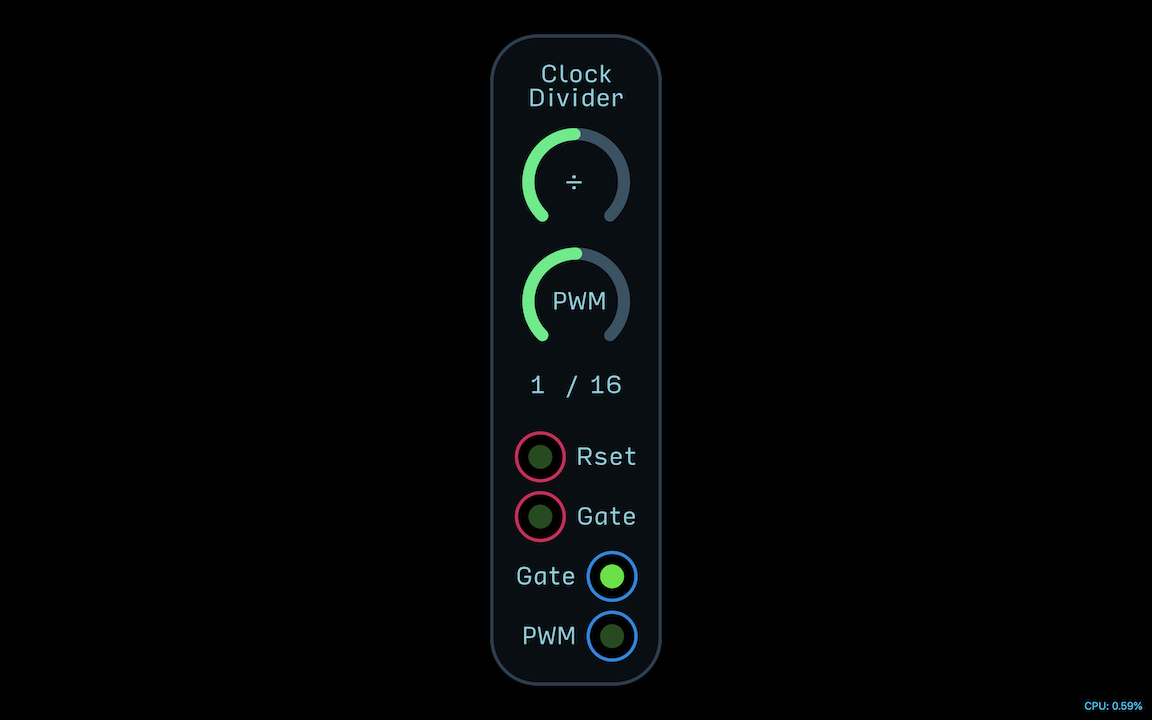
\includegraphics[width=\textwidth]{clock-divider.png}

\begin{table}[ht]
\small
\sffamily
\renewcommand\arraystretch{1.5}
\centering
\begin{tabular}{l*{1}{>{\raggedright\arraybackslash}p{0.7\linewidth}}}

\toprule
\textbf{Knob} \\
$\div$ & \textit{Sets clock speed divide-by factor from 1/1 to 1/64.} \\
PWM & \textit{Sets the pulse width of the divided clock at the PWM output. Does not effect the Gate output.} \\

\midrule
\textbf{Input} \\
Rset & \textit{Gate this input to reset the divide-by counter. Useful when attempting to sync multiple Clock Divider modules.} \\
Gate & \textit{Connect the clock signal you want to divide to this input.} \\

\midrule
\textbf{Output} \\
Gate & \textit{The divided gate signal output. This gate output will preserve the pulse width of the incoming gate signal.} \\
PWM & \textit{The divided gate signal output. This gate output will have a pulse width set by the PWM knob.} \\

\bottomrule
\end{tabular}
\end{table}% \\

\pagebreak


\section{Master Clock}

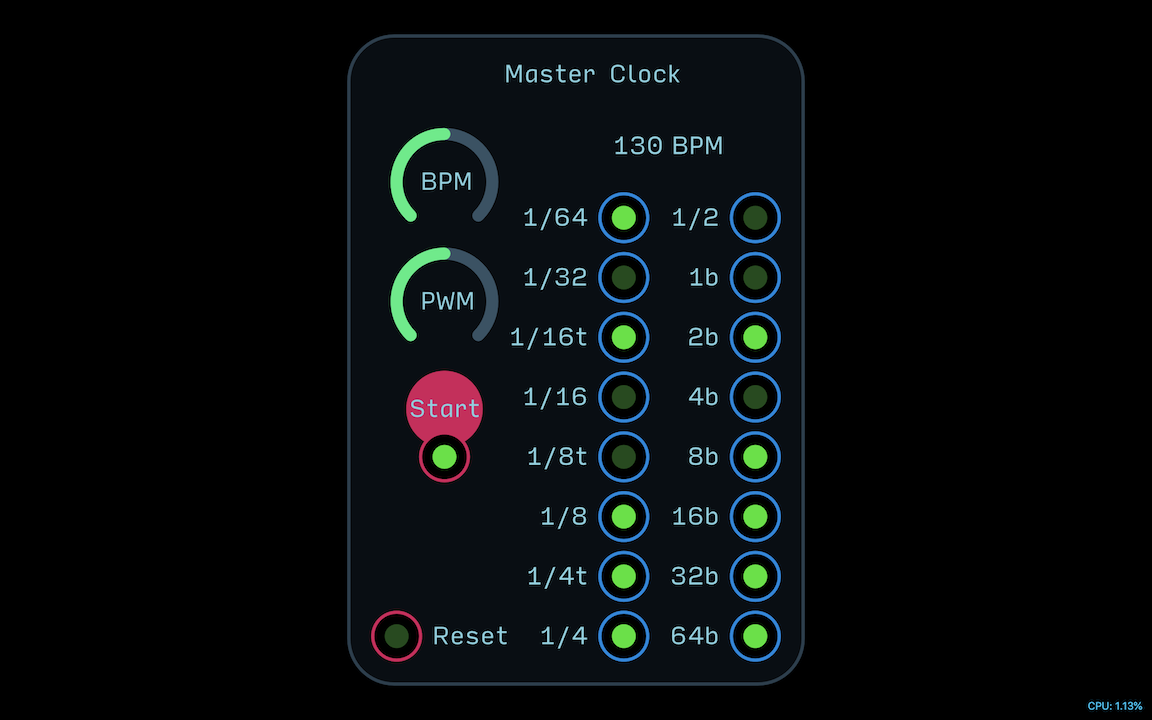
\includegraphics[width=\textwidth]{master-clock.png}

\begin{table}[ht]
\small
\sffamily
\renewcommand\arraystretch{1.5}
\centering
\begin{tabular}{l*{1}{>{\raggedright\arraybackslash}p{0.7\linewidth}}}

\toprule
\textbf{Knob} \\
BPM & \textit{Sets the beats per minute (BPM) of the clock from 60 to 220 in steps of 1BPM.} \\
PWM & \textit{Sets the pulse width of all outputs simultaneously.} \\

\midrule
\textbf{Button} \\
Start & \textit{Press to start and stop the clock. Clock will reset when restarted. Gate input below will remotely turn clock on and off so long as the button itself is off.} \\

\midrule
\textbf{Input} \\
Reset & \textit{Gate this input to reset the clock.} \\

\midrule
\textbf{Output} \\
1/$x$ & \textit{Subdivided clock outputs, e.g. 1/16 = 16th note.} \\
1/$x$t & \textit{Subdivided triplet clock outputs, e.g. 1/8t = 8th note triplet.} \\
$x$b & \textit{Bar multiples of clock, e.g. 32b = 32 bars.} \\


\bottomrule
\end{tabular}
\end{table}% \\

\pagebreak


\section{Bernoulli Gate}

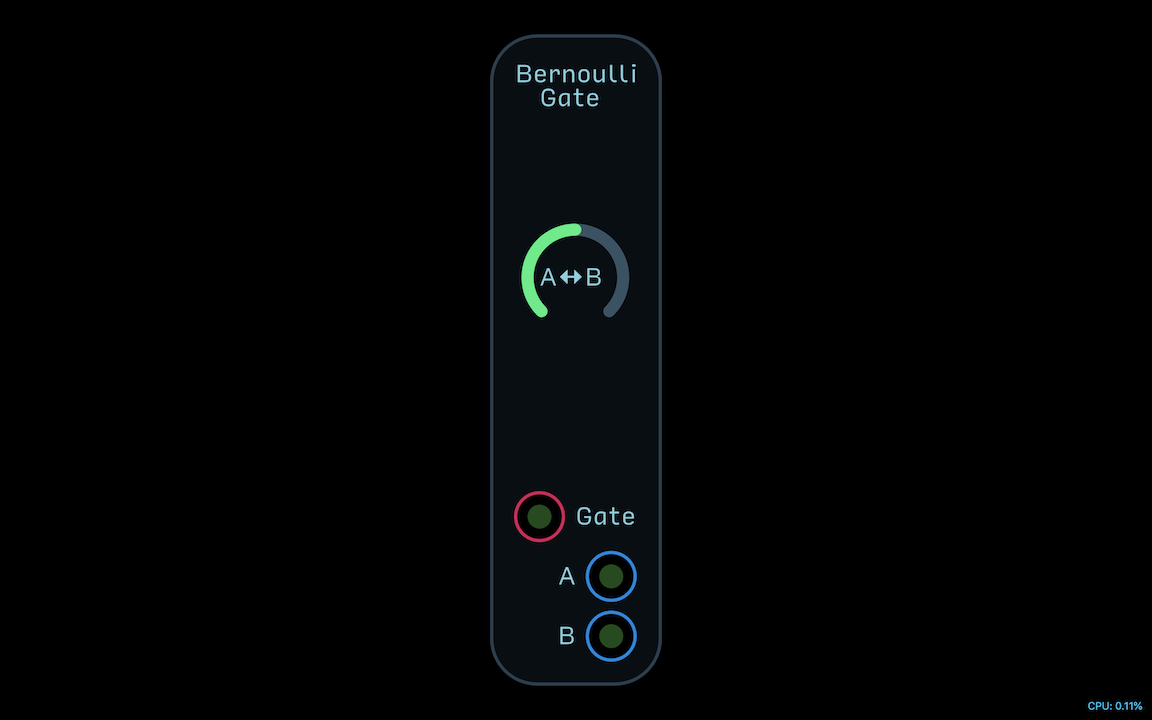
\includegraphics[width=\textwidth]{bernoulli-gate.png}

\begin{table}[ht]
\small
\sffamily
\renewcommand\arraystretch{1.5}
\centering
\begin{tabular}{l*{1}{>{\raggedright\arraybackslash}p{0.7\linewidth}}}

\toprule
\textbf{Knob} \\
A$\leftrightarrow$B & \textit{Sets the chance that the incoming gate will be sent to either output A or output B. If knob is set in the middle, there is a 50\% chance of A or B being chosen. If set all the way left, then A will be chosen 100\% of the time. If set all the way to the right, B will be chosen 100\% of the time.} \\

\midrule
\textbf{Input} \\
Gate & \textit{The gate or clock signal you wish to randomly distribute to output A or B.} \\

\midrule
\textbf{Output} \\
A/B& \textit{Outputs a gate if chosen depending on random chance biased by A$\leftrightarrow$B knob.} \\

\bottomrule
\end{tabular}
\end{table}% \\

\pagebreak


\section{Chance Select Gate}

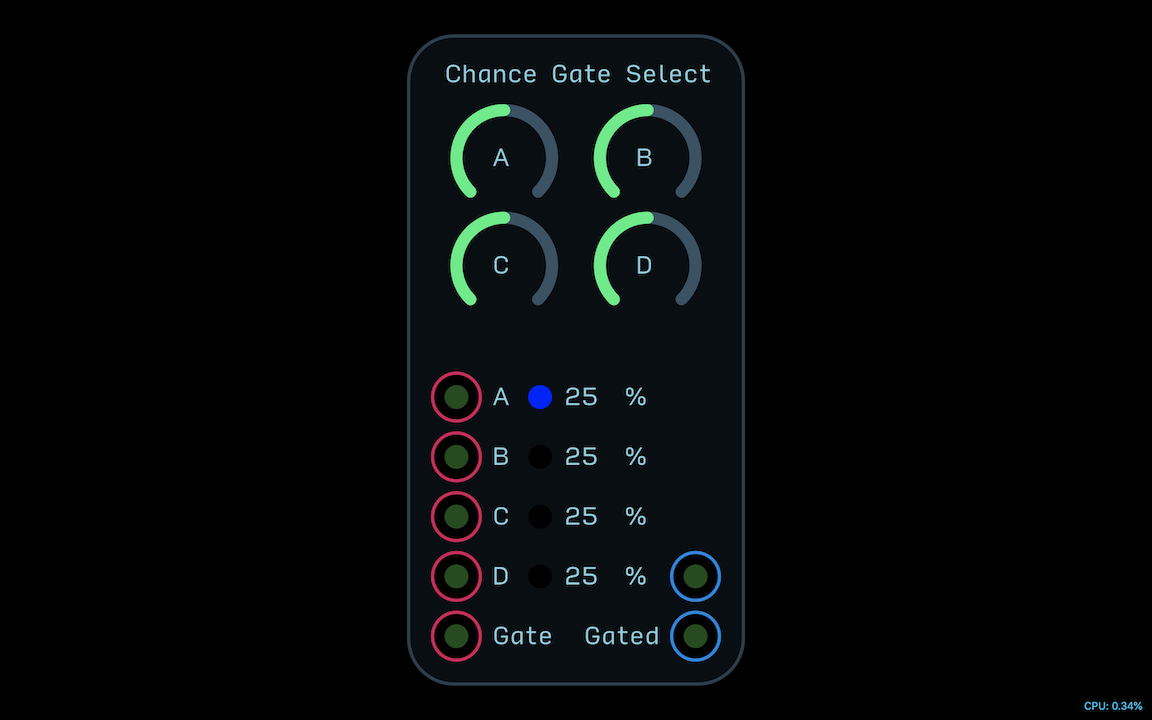
\includegraphics[width=\textwidth]{chance-select-gate.png}

\begin{table}[ht]
\small
\sffamily
\renewcommand\arraystretch{1.5}
\centering
\begin{tabular}{l*{1}{>{\raggedright\arraybackslash}p{0.7\linewidth}}}

\toprule
\textbf{Knob} \\
A/B/C/D & \textit{Each knob sets the chance that their corresponding input will be chosen when the module is gated at the \textnormal{Gate} input.} \\

\midrule
\textbf{Input} \\
A/B/C/D & \textit{Input gates or clock signals to be chosen from.} \\
Gate & \textit{Gate this input to trigger a new choice between inputs A/B/C/D.} \\

\midrule
\textbf{Output} \\
A/B& \textit{Outputs a gate if chosen depending on random chance biased by A$\leftrightarrow$B knob.} \\

\bottomrule
\end{tabular}
\end{table}% \\

\pagebreak


\section{Pachinko Machine}

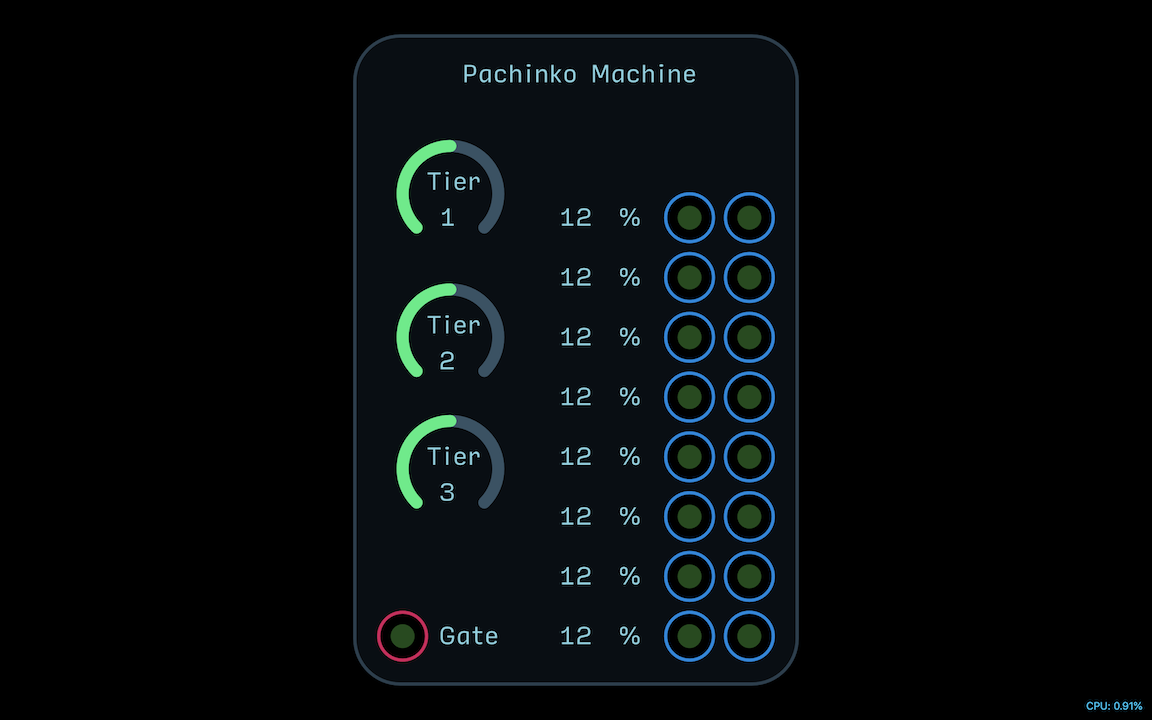
\includegraphics[width=\textwidth]{pachinko-machine.png}

\begin{table}[ht]
\small
\sffamily
\renewcommand\arraystretch{1.5}
\centering
\begin{tabular}{l*{1}{>{\raggedright\arraybackslash}p{0.7\linewidth}}}

\toprule
\textbf{Knob} \\
Tier 1/2/3 & \textit{Sets the balance of probability of each subsequent tier of Bernoulli Gate modules. Tier 1 has x1, Tier 2 has x2, and Tier 3 has x4.} \\

\midrule
\textbf{Input} \\
Gate & \textit{Gating this input is like launching a  ball to the top of the Pachinko machine. Where the gate exits depends on the probability of each tier, indicated by the displays next to each output.} \\

\midrule
\textbf{Output} \\
Left Column Gates & \textit{Outputs the incoming gate if selected by chance.} \\
Right Column Gates & \textit{Outputs the incoming gate if selected by chance and stays high until selected again when it then goes low.} \\

\bottomrule
\end{tabular}
\end{table}% \\

\pagebreak


\section{Random Bursts}

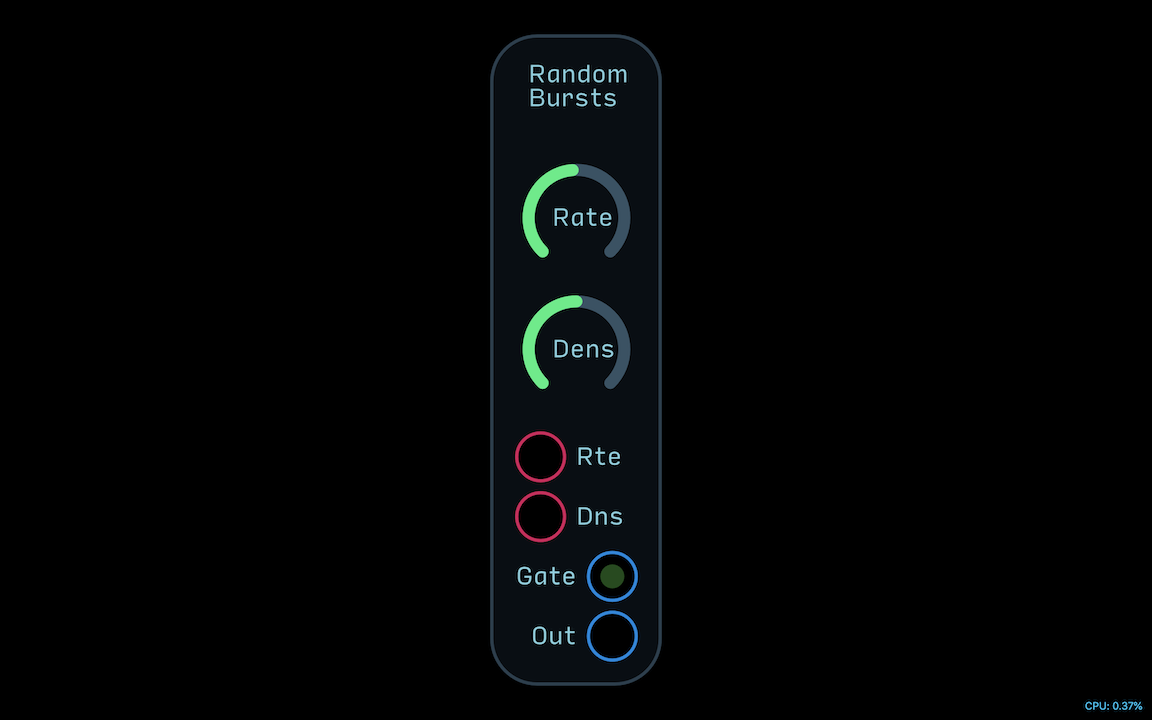
\includegraphics[width=\textwidth]{random-bursts.png}

\begin{table}[ht]
\small
\sffamily
\renewcommand\arraystretch{1.5}
\centering
\begin{tabular}{l*{1}{>{\raggedright\arraybackslash}p{0.7\linewidth}}}

\toprule
\textbf{Knob} \\
Rate & \textit{Sets the speed at which random bursts happen.} \\
Dens & \textit{Sets how densely grouped the random bursts are.} \\

\midrule
\textbf{Input} \\
Rte & \textit{Modulation input for Rate.} \\
Dns & \textit{Modulation input for Density.} \\

\midrule
\textbf{Output} \\
Gate & \textit{Outputs random bursts of gates.} \\
Out & \textit{Outputs random bursts of bipolar white noise.} \\

\bottomrule
\end{tabular}
\end{table}% \\

\pagebreak


\section{uClock}

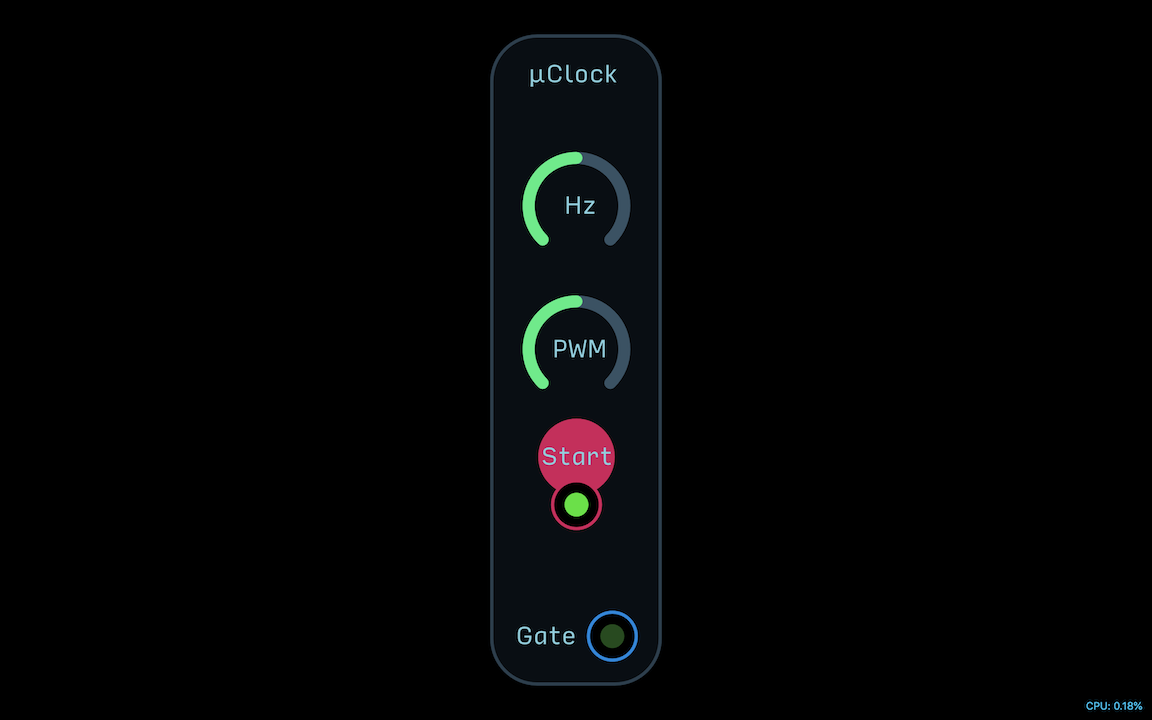
\includegraphics[width=\textwidth]{uclock.png}

\begin{table}[ht]
\small
\sffamily
\renewcommand\arraystretch{1.5}
\centering
\begin{tabular}{l*{1}{>{\raggedright\arraybackslash}p{0.7\linewidth}}}

\toprule
\textbf{Knob} \\
Hz & \textit{Sets the speed of the clock from 0 to 20Hz.} \\
PWM & \textit{Sets the pulse width of the clock from 0 to 100\%.} \\

\midrule
\textbf{Button} \\
Start & \textit{Press to start and stop the clock. Clock will reset when restarted. Gate input below will remotely turn clock on and off so long as the button itself is off.} \\

\midrule
\textbf{Output} \\
Gate & \textit{Clock output.} \\

\bottomrule
\end{tabular}
\end{table}% \\

\pagebreak


\chapter{Drum Modules}
\pagebreak

\section{Percussion}

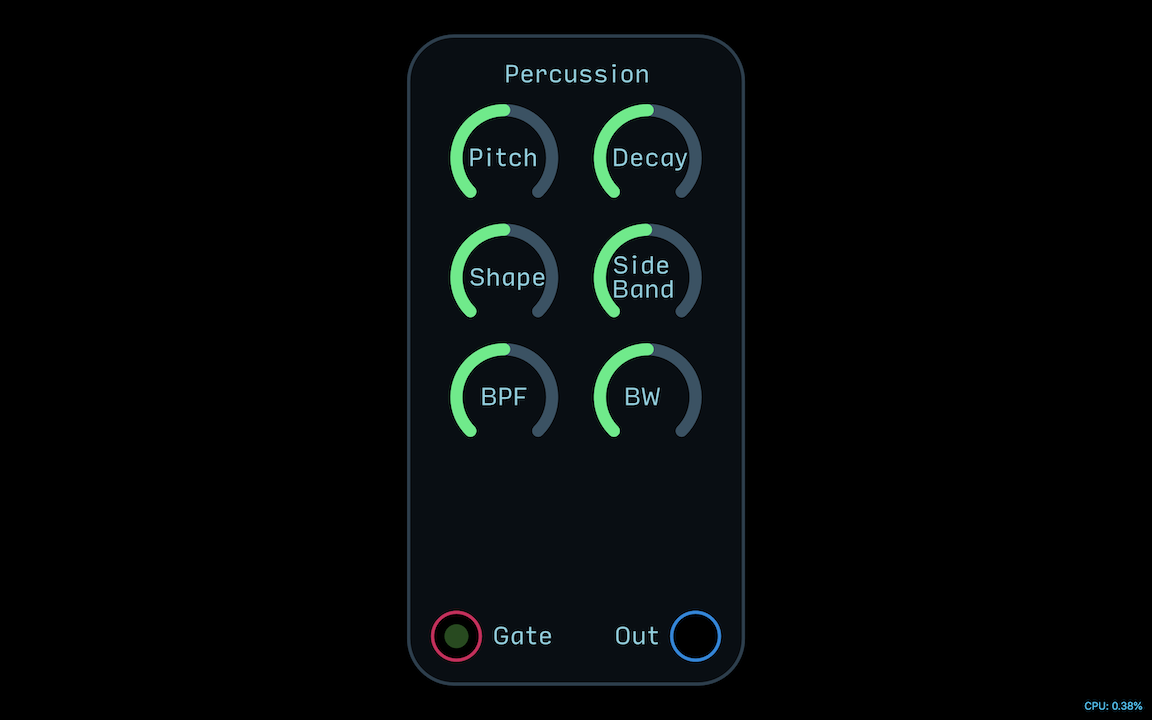
\includegraphics[width=\textwidth]{percussion.png}

\begin{table}[ht]
\small
\sffamily
\renewcommand\arraystretch{1.5}
\centering
\begin{tabular}{l*{1}{>{\raggedright\arraybackslash}p{0.7\linewidth}}}

\toprule
\textbf{Knob} \\
Pitch & \textit{Sets the pitch of the oscillators.} \\
Decay & \textit{Controls the length of decay. If turned all the way up, the sound will stay on indefinitely.} \\
Shape & \textit{Fades oscillator shape from sine to triangle. Interactive with the Side Band control as the oscillators cross-modulate one another.} \\
Side Band & \textit{Fades from pure oscillators to ring modulation through to a kind of digital modulation.} \\
BPF & \textit{Adjusts the frequency center of the bandpass filter.} \\
BW & \textit{Controls the bandwidth of the bandpass filter. Higher settings mean more bandwidth.} \\

\midrule
\textbf{Input} \\
Gate & \textit{Triggers drum sound.} \\

\midrule
\textbf{Output} \\
Out & \textit{Audio output.} \\

\bottomrule
\end{tabular}
\end{table}% \\

\pagebreak


\section{$\mu$Hat}

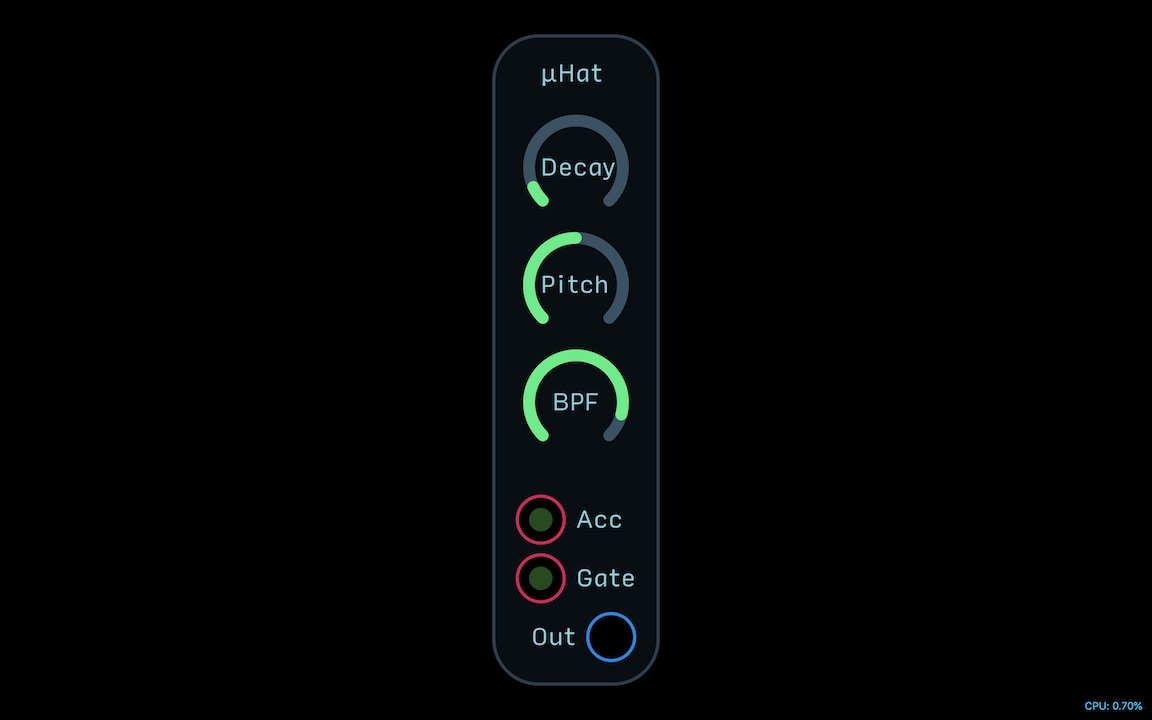
\includegraphics[width=\textwidth]{uhat.png}

\begin{table}[ht]
\small
\sffamily
\renewcommand\arraystretch{1.5}
\centering
\begin{tabular}{l*{1}{>{\raggedright\arraybackslash}p{0.7\linewidth}}}

\toprule
\textbf{Knob} \\
Decay & \textit{Controls the length of decay.} \\
Pitch & \textit{Sets the pitch of the hat.} \\
BPF & \textit{Fades oscillator shape from sine to triangle.} \\

\midrule
\textbf{Input} \\
Acc & \textit{When gated, the Accent input increases the decay time of the module, allowing for an open hat sound. The amount of decay time increase can be adjusted internally with a trimpot control.} \\
Gate & \textit{Triggers drum sound.} \\

\midrule
\textbf{Output} \\
Out & \textit{Audio output.} \\

\bottomrule
\end{tabular}
\end{table}% \\

\pagebreak


\section{$\mu$Kick}

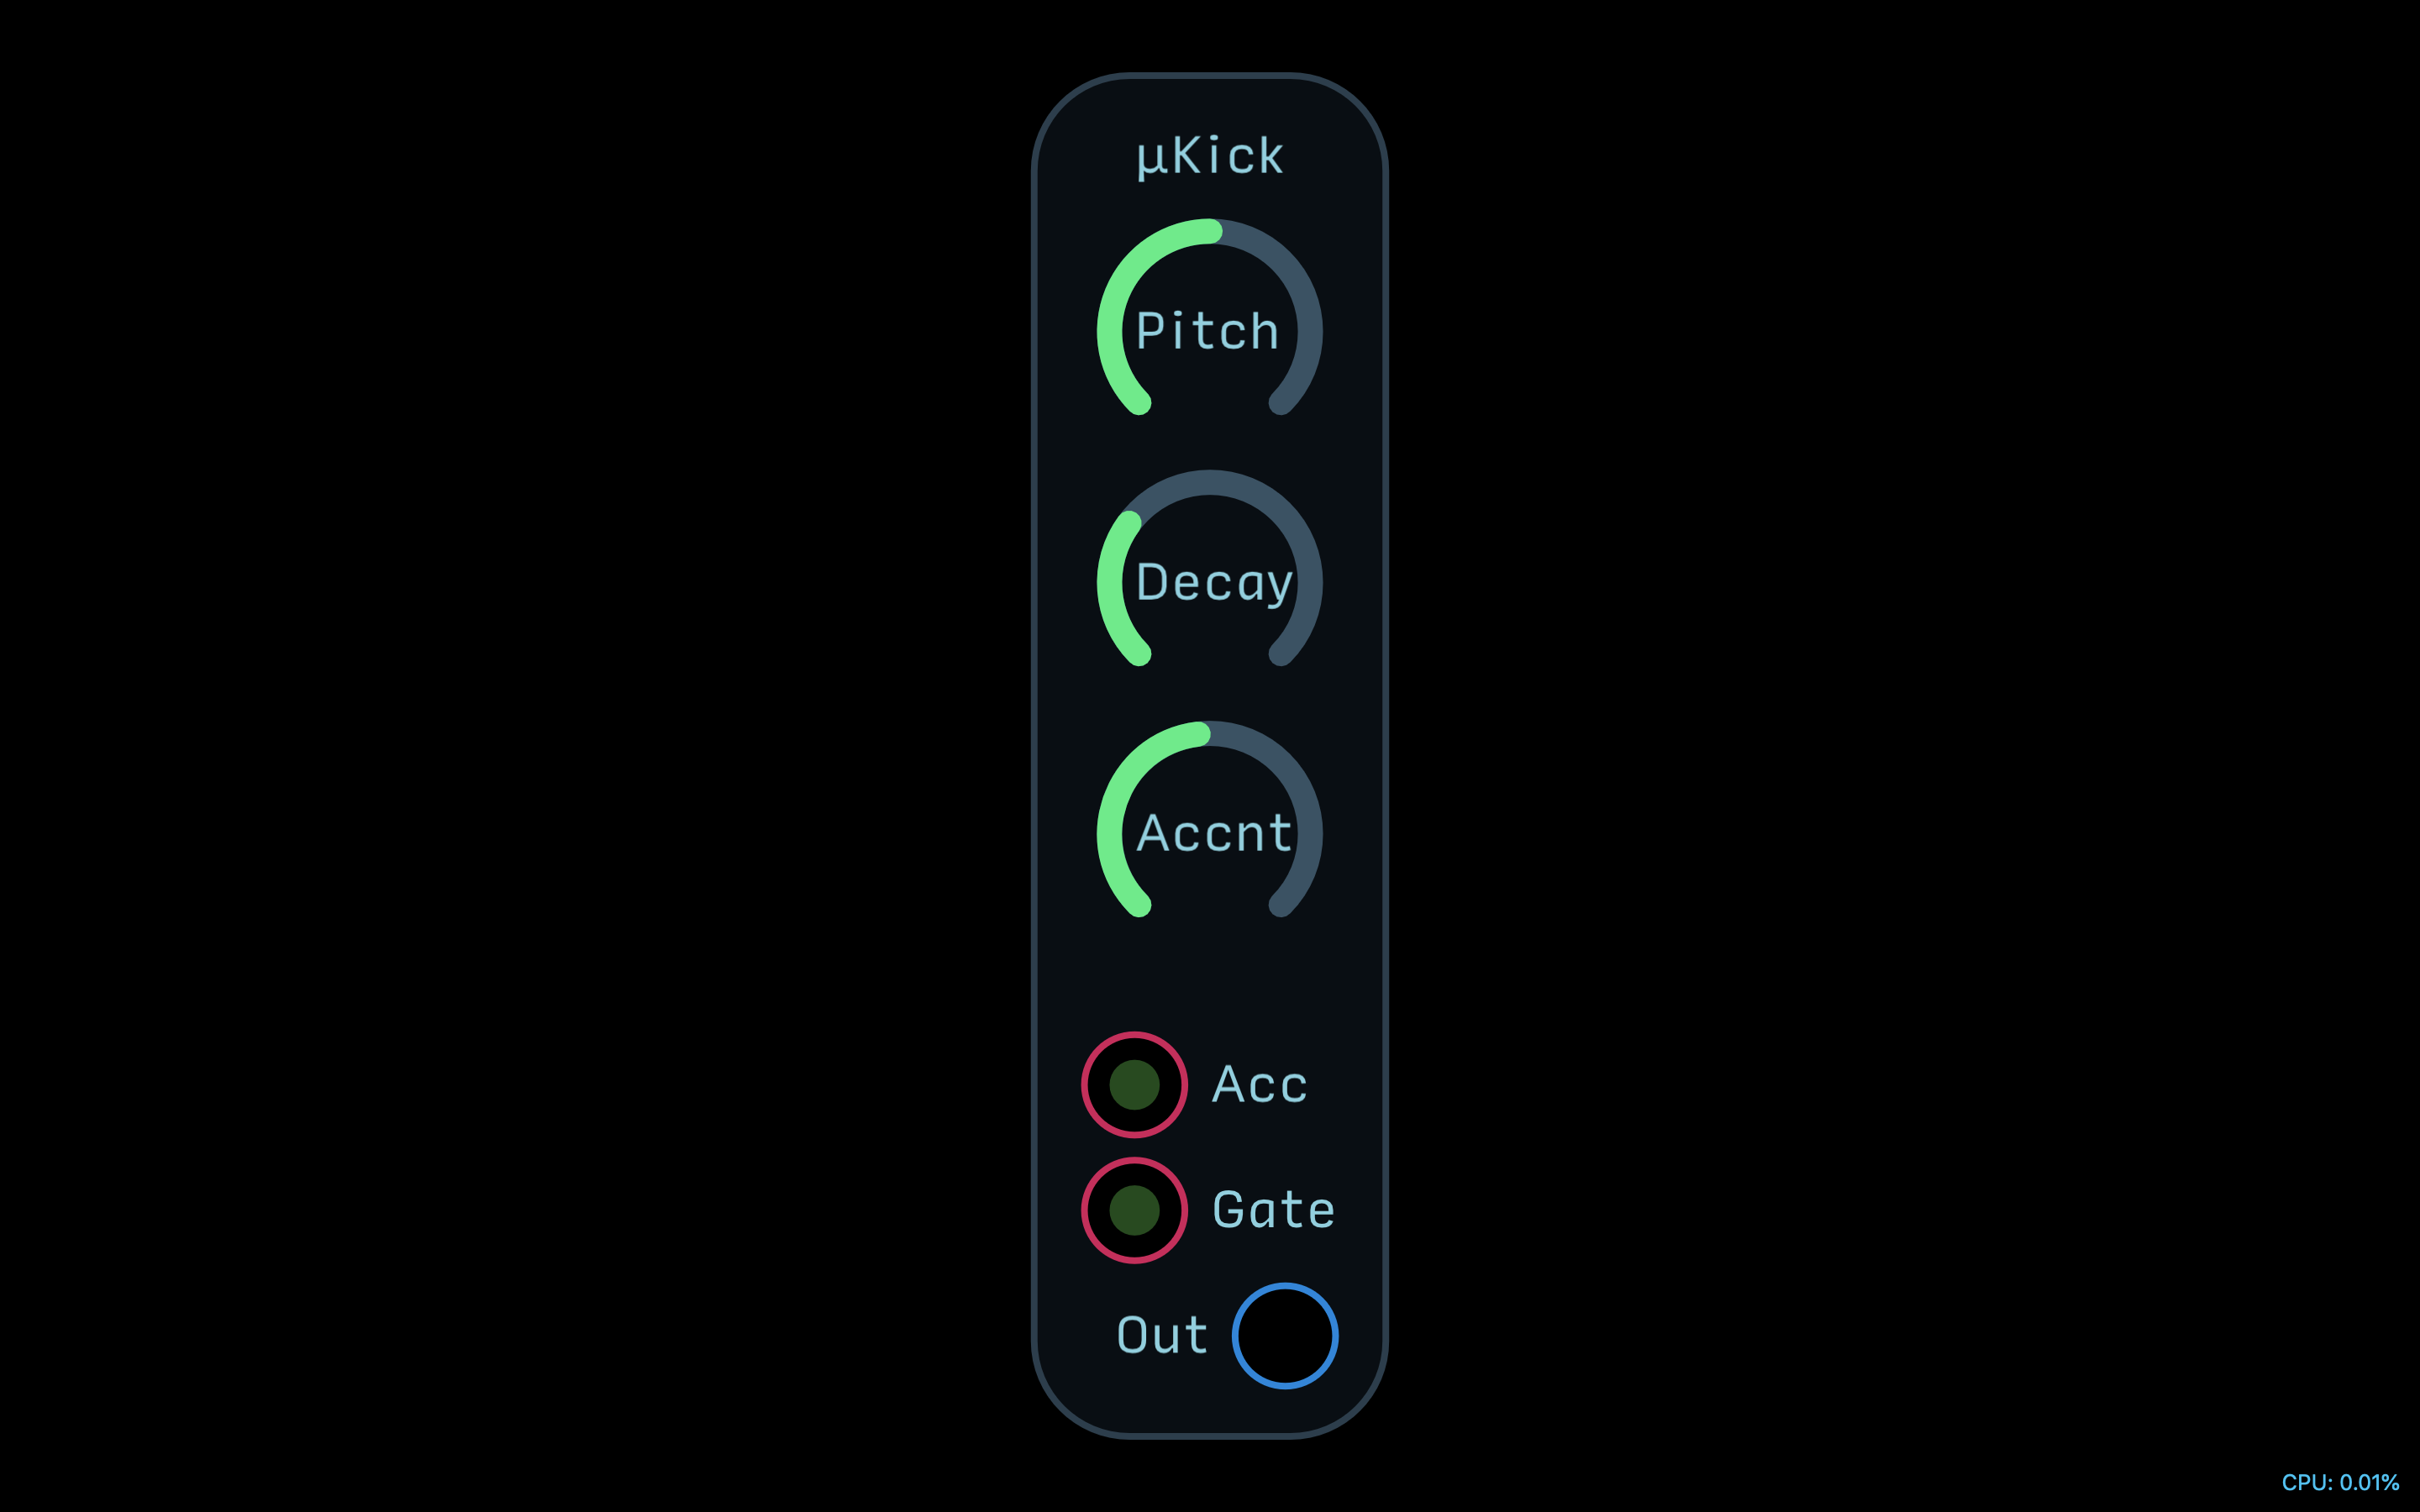
\includegraphics[width=\textwidth]{ukick.png}

\begin{table}[ht]
\small
\sffamily
\renewcommand\arraystretch{1.5}
\centering
\begin{tabular}{l*{1}{>{\raggedright\arraybackslash}p{0.7\linewidth}}}

\toprule
\textbf{Knob} \\
Pitch & \textit{Sets the upper pitch the kick decays from.} \\
Decay & \textit{Sets the decay time of the kick.} \\
Accnt & \textit{Normalized accent control that, when turned up, actually lowers the volume of the unaccented sound relative to the accented sound.} \\

\midrule
\textbf{Input} \\
Acc & \textit{When gated, the Accent input increases the volume of the drum as long as the Accnt control is turned up.} \\
Gate & \textit{Triggers drum sound.} \\

\midrule
\textbf{Output} \\
Out & \textit{Audio output.} \\

\bottomrule
\end{tabular}
\end{table}% \\

\pagebreak


\section{$\mu$Snare}

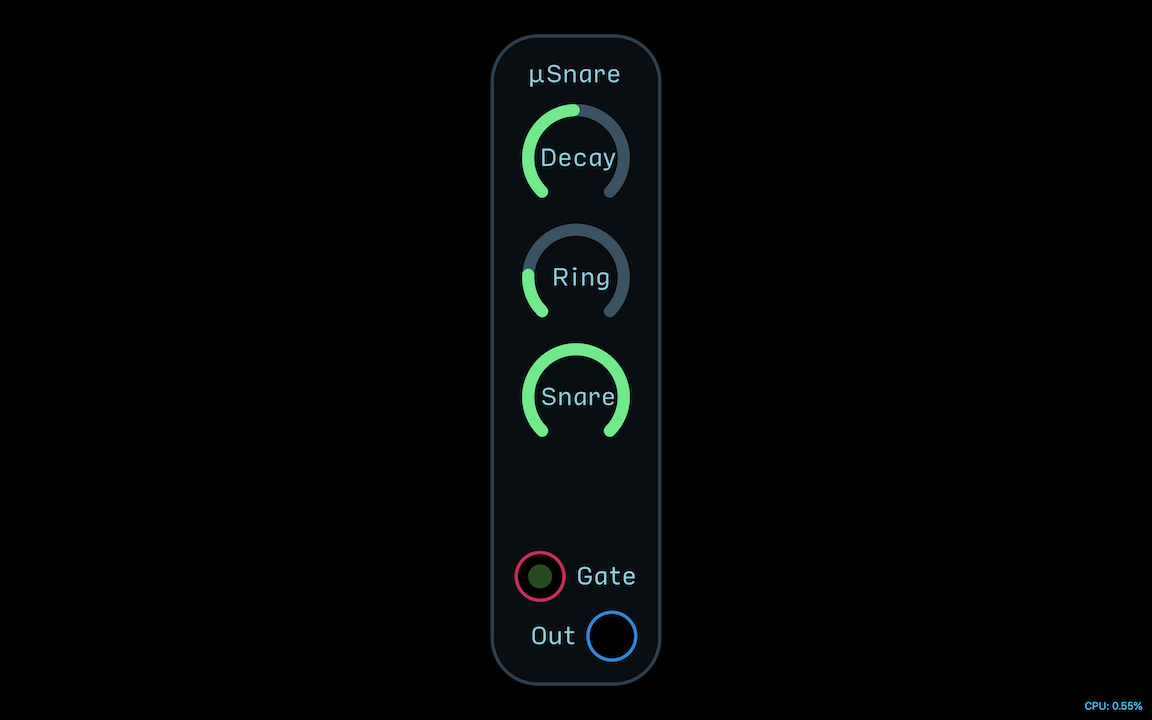
\includegraphics[width=\textwidth]{usnare.png}

\begin{table}[ht]
\small
\sffamily
\renewcommand\arraystretch{1.5}
\centering
\begin{tabular}{l*{1}{>{\raggedright\arraybackslash}p{0.7\linewidth}}}

\toprule
\textbf{Knob} \\
Decay & \textit{Sets the decay time of the snare.} \\
Ring & \textit{Adjusts the loudness of the ringing fundamental tone.} \\
Snare & \textit{Sets the loudness of the noise component of the drum known as the snares.} \\

\midrule
\textbf{Input} \\
Gate & \textit{Triggers drum sound.} \\

\midrule
\textbf{Output} \\
Out & \textit{Audio output.} \\

\bottomrule
\end{tabular}
\end{table}% \\

\pagebreak


\chapter{Effect Modules}
\pagebreak

\section{Delay}
\pagebreak

\subsection{Stereo Delay}

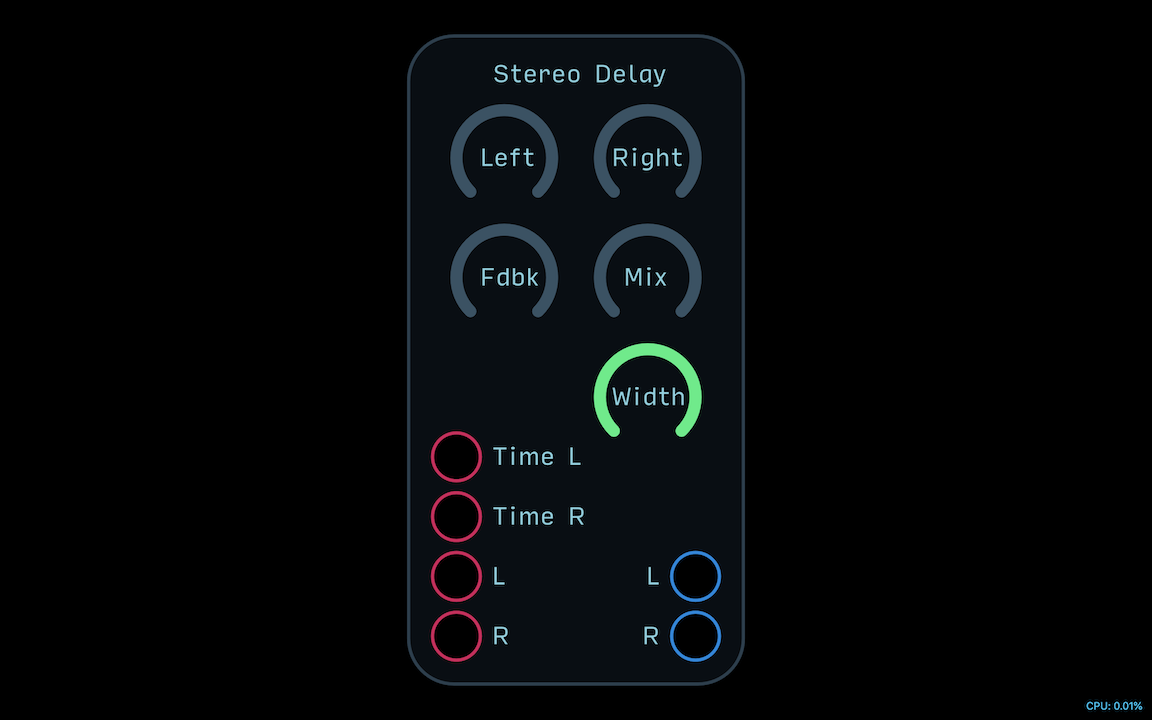
\includegraphics[width=\textwidth]{stereo-delay.png}

\begin{table}[ht]
\small
\sffamily
\renewcommand\arraystretch{1.5}
\centering
\begin{tabular}{l*{1}{>{\raggedright\arraybackslash}p{0.7\linewidth}}}

\toprule
\textbf{Knob} \\
Left/Right & \textit{Sets the delay time for the Left/Right channels.} \\
Fdbk & \textit{Sets the amount of feedback for both channels.} \\
Mix & \textit{Balances the wet/dry mix.} \\
Width & \textit{Adjusts the stereo separation of delays from mono to stereo.} \\

\midrule
\textbf{Input} \\
Time L/R & \textit{Time inputs for the sync module. You can also use them as modulation inputs to create vibrato or chorus effects.} \\
L/R & \textit{Stereo audio inputs for Left and Right channels.} \\

\midrule
\textbf{Output} \\
L/R & \textit{Stereo audio outputs for Left and Right channels.} \\

\bottomrule
\end{tabular}
\end{table}% \\

\pagebreak


\subsection{Delay Looper Sync}

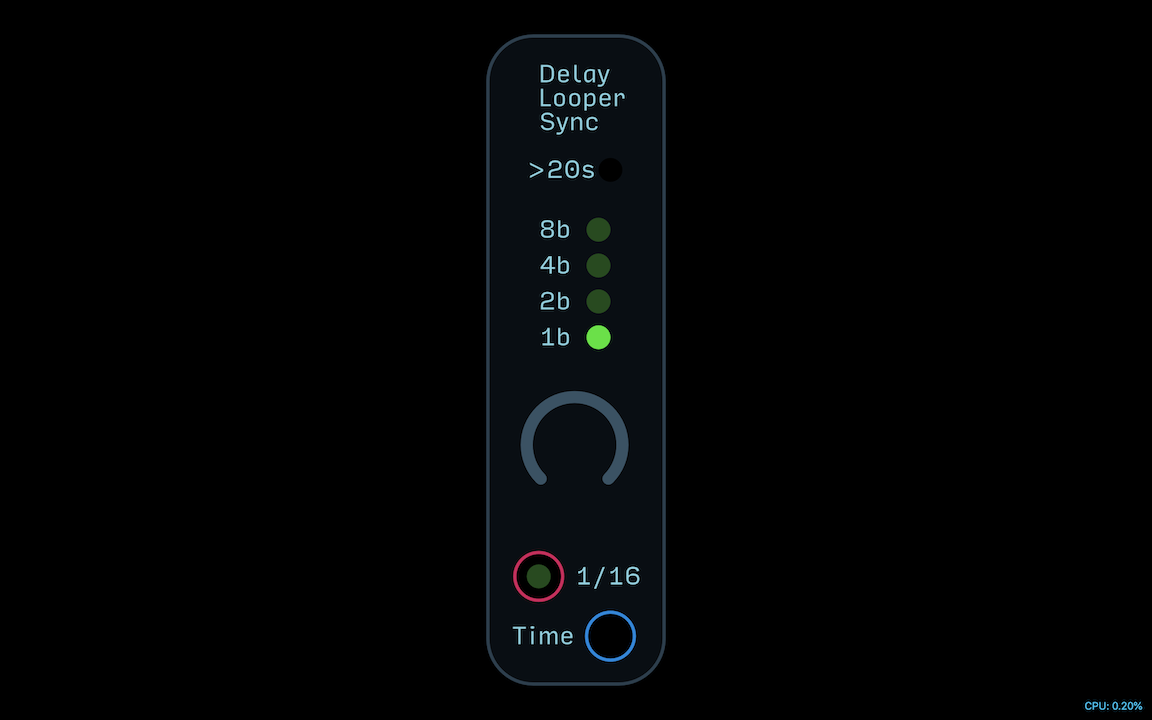
\includegraphics[width=\textwidth]{delay-looper-sync.png}

\begin{table}[ht]
\small
\sffamily
\renewcommand\arraystretch{1.5}
\centering
\begin{tabular}{l*{1}{>{\raggedright\arraybackslash}p{0.7\linewidth}}}

\toprule
\textbf{Knob} \\
Unlabeled knob & \textit{Switches between 1, 2, 4, or 8 bars of loop time. If total loop time exceeds the maximum 20 seconds of the Delay node, a red light will appear at the top.} \\

\midrule
\textbf{Input} \\
1/16 & \textit{Gate input for syncing that expects a 1/16th note pulse. Use the 1/16th note output of the Master Clock module for consistent results.} \\

\midrule
\textbf{Output} \\
Time & \textit{Outputs the number of seconds of loop time. Connect only to the Time inputs of delay modules.} \\

\bottomrule
\end{tabular}
\end{table}% \\

\pagebreak


\subsection{Delay Tempo Sync}

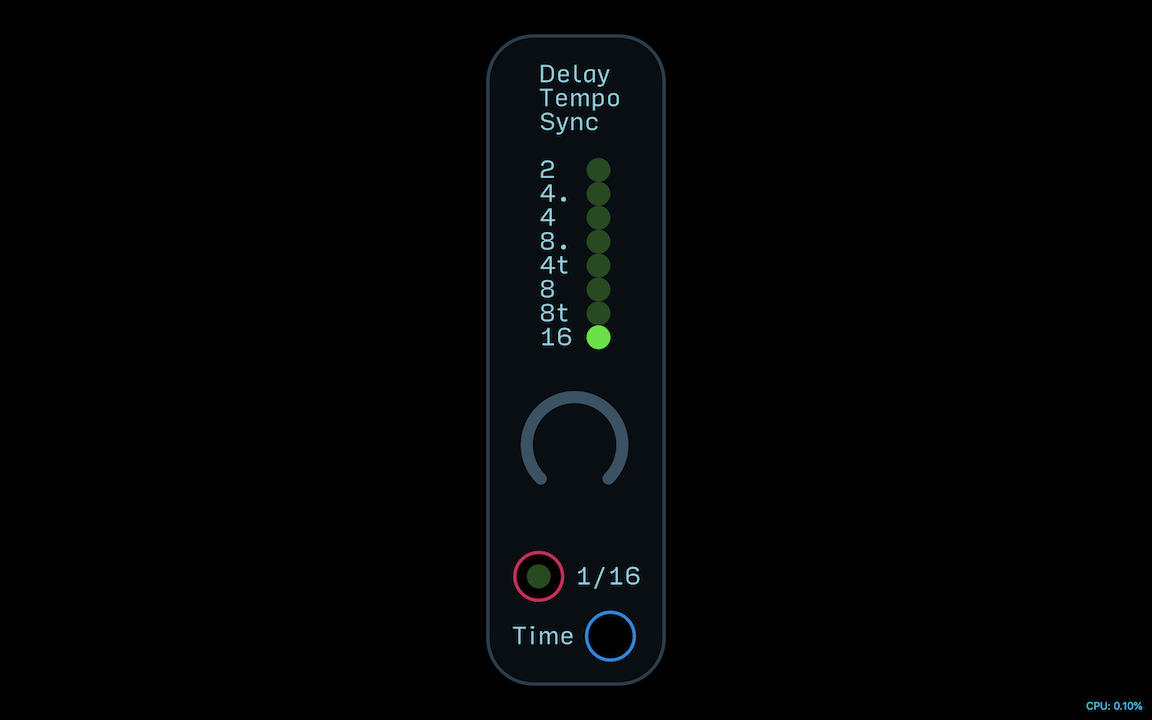
\includegraphics[width=\textwidth]{delay-tempo-sync.png}

\begin{table}[ht]
\small
\sffamily
\renewcommand\arraystretch{1.5}
\centering
\begin{tabular}{l*{1}{>{\raggedright\arraybackslash}p{0.7\linewidth}}}

\toprule
\textbf{Knob} \\
Unlabeled knob & \textit{Switches between subdivisions of delay time. Top to bottom: 1/2, 1/4 dotted, 1/4, 1/8th dotted, 1/4 triplet, 1/8th, 1/8th triplet, 16th. If total delay time exceeds the maximum 20 seconds of the Delay node, a red light will appear at the top.} \\

\midrule
\textbf{Input} \\
1/16 & \textit{Gate input for syncing that expects a 1/16th note pulse. Use the 1/16th note output of the Master Clock module for consistent results.} \\

\midrule
\textbf{Output} \\
Time & \textit{Outputs the number of seconds of loop time. Connect only to the Time inputs of delay modules.} \\

\bottomrule
\end{tabular}
\end{table}% \\

\pagebreak


\subsection{uDelay}

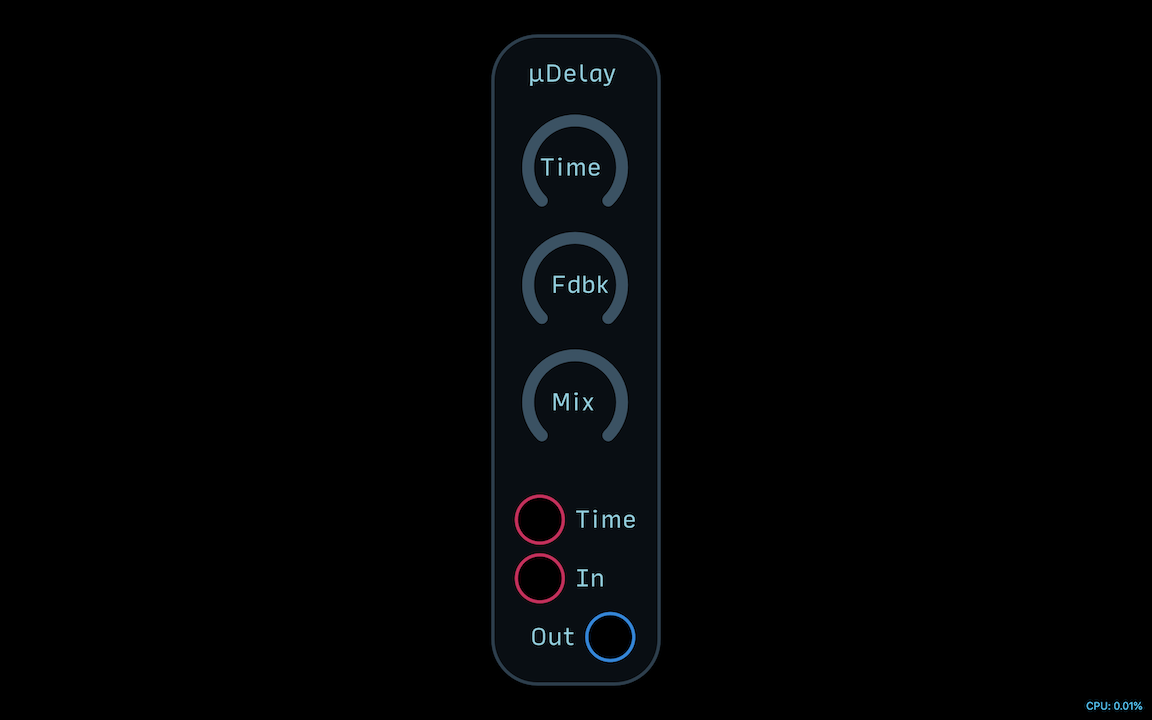
\includegraphics[width=\textwidth]{udelay.png}

\begin{table}[ht]
\small
\sffamily
\renewcommand\arraystretch{1.5}
\centering
\begin{tabular}{l*{1}{>{\raggedright\arraybackslash}p{0.7\linewidth}}}

\toprule
\textbf{Knob} \\
Time & \textit{Sets the delay time.} \\
Fdbk & \textit{Sets the amount of feedback.} \\
Mix & \textit{Balances the wet/dry mix.} \\

\midrule
\textbf{Input} \\
Time & \textit{Time input for the sync module. You can also use it as a modulation input to create vibrato or chorus effects.} \\
In & \textit{Audio input.} \\

\midrule
\textbf{Output} \\
Out & \textit{Audio output.} \\

\bottomrule
\end{tabular}
\end{table}% \\

\pagebreak


\section{Distortion}
\pagebreak

\subsection{Asymmetrical Drive}

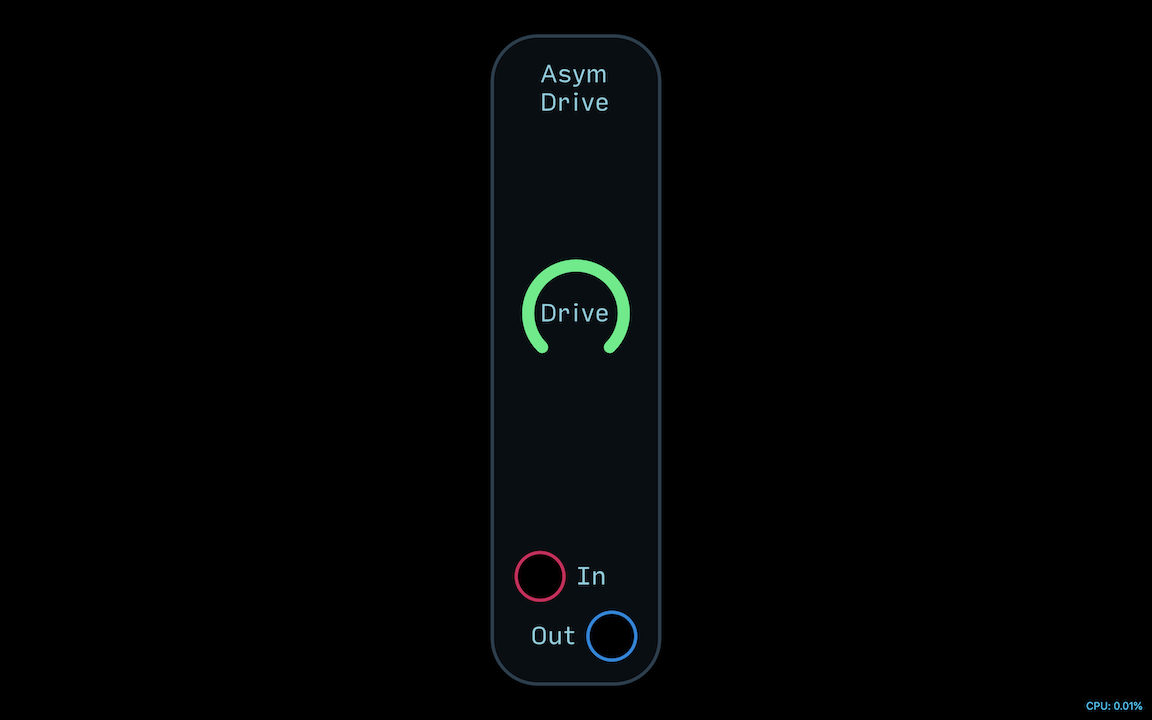
\includegraphics[width=\textwidth]{asymmetrical-drive.png}

\begin{table}[ht]
\small
\sffamily
\renewcommand\arraystretch{1.5}
\centering
\begin{tabular}{l*{1}{>{\raggedright\arraybackslash}p{0.7\linewidth}}}

\toprule
\textbf{Knob} \\
Drive & \textit{Sets the amount of distortion.} \\

\midrule
\textbf{Input} \\
In & \textit{Audio input.} \\

\midrule
\textbf{Output} \\
Out & \textit{Audio output.} \\

\bottomrule
\end{tabular}
\end{table}% \\

\pagebreak


\subsection{Fold Processor}

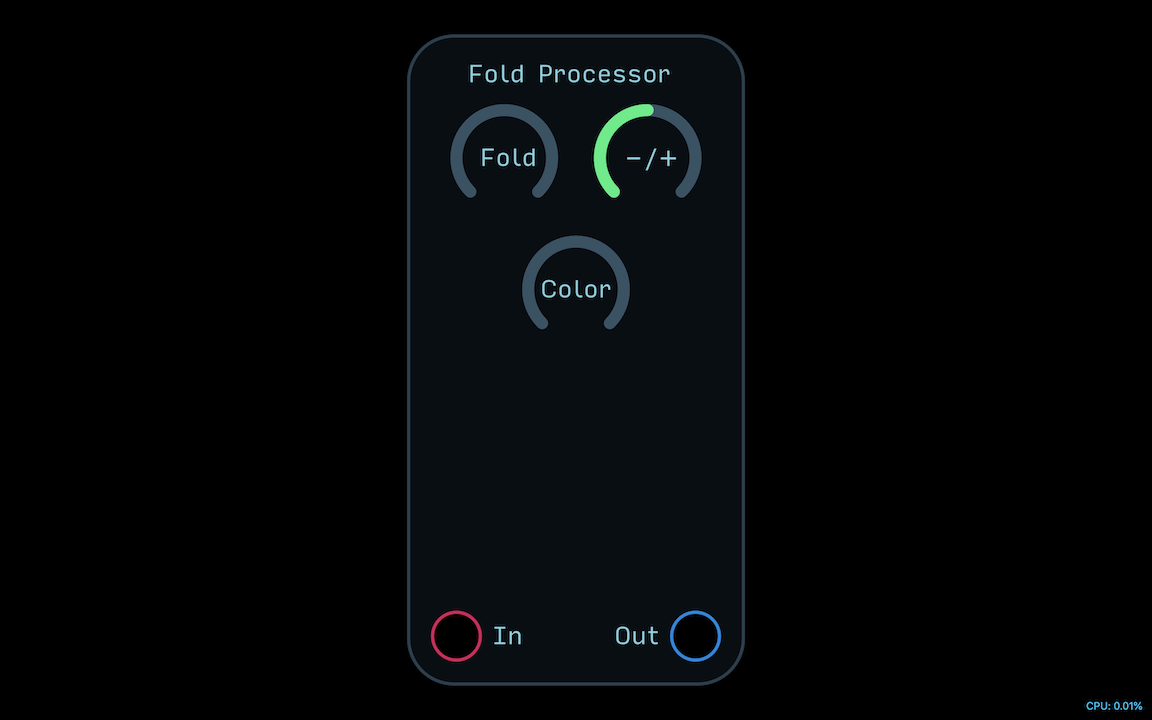
\includegraphics[width=\textwidth]{fold-processor.png}

\begin{table}[ht]
\small
\sffamily
\renewcommand\arraystretch{1.5}
\centering
\begin{tabular}{l*{1}{>{\raggedright\arraybackslash}p{0.7\linewidth}}}

\toprule
\textbf{Knob} \\
Fold & \textit{Amplifies the incoming audio as it enters the wavefolding section} \\
-/+ & \textit{Offset control that will add or subtract an offset factor as it enters the wavefolding section.} \\
Color & \textit{Fades between simple and more complex wavefolding.} \\

\midrule
\textbf{Input} \\
In & \textit{Audio input.} \\

\midrule
\textbf{Output} \\
Out & \textit{Audio output.} \\

\bottomrule
\end{tabular}
\end{table}% \\

\pagebreak


\section{Reverb}
\pagebreak

\subsection{Really Humungous Reverb}

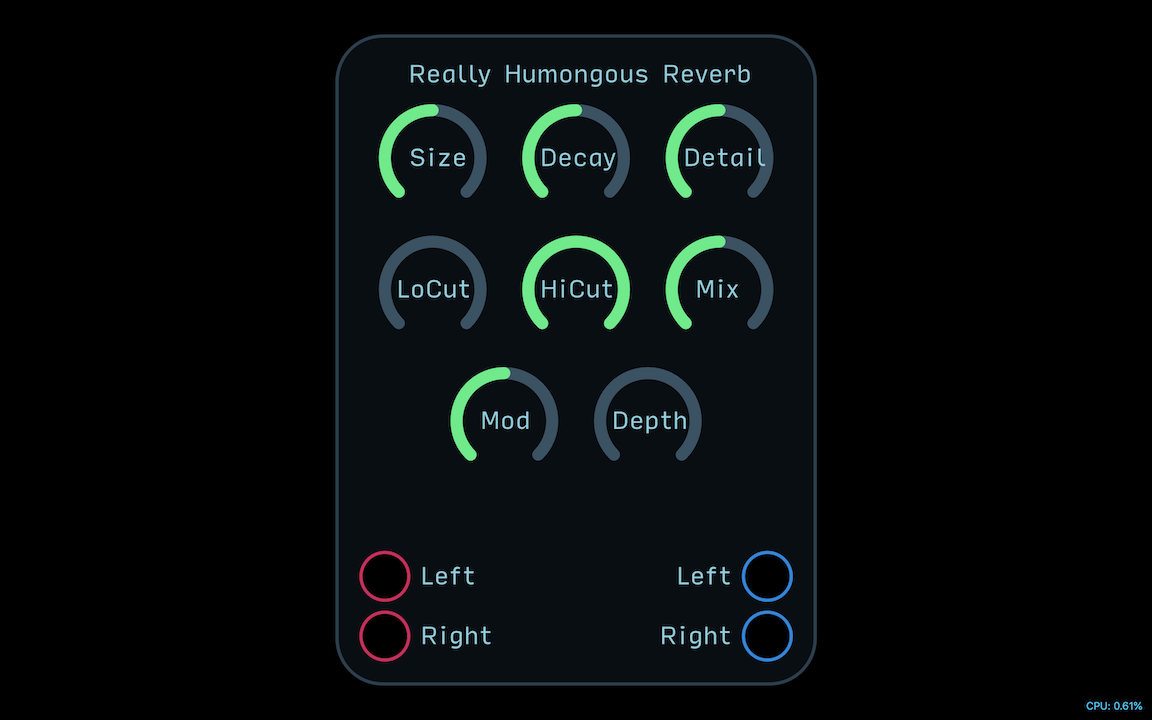
\includegraphics[width=\textwidth]{really-humongous-reverb.png}

\begin{table}[ht]
\small
\sffamily
\renewcommand\arraystretch{1.5}
\centering
\begin{tabular}{l*{1}{>{\raggedright\arraybackslash}p{0.7\linewidth}}}

\toprule
\textbf{Knob} \\
Size & \textit{Adjusts the percieved size of the virtual room from big to enormous.} \\
Decay & \textit{Sets the decay time of the reverberations.} \\
Detail & \textit{Adjusts the crispness of the reverberations.} \\
LoCut & \textit{Cuts off low frequencies. Good for tightening up reverb by removing muddy bass.} \\
HiCut & \textit{Cuts off high frequencies. Good for smoothing out reverb to make it more realistic.} \\
Mix & \textit{Adjusts the wet/dry balance.} \\
Mod & \textit{Adjusts Size modulation speed.} \\
Depth & \textit{Adjusts Size modulation amount.} \\

\midrule
\textbf{Input} \\
Left/Right & \textit{Stereo audio input.} \\

\midrule
\textbf{Output} \\
Left/Right & \textit{Stereo audio output.} \\

\bottomrule
\end{tabular}
\end{table}% \\

\pagebreak


\subsection{uVerb}

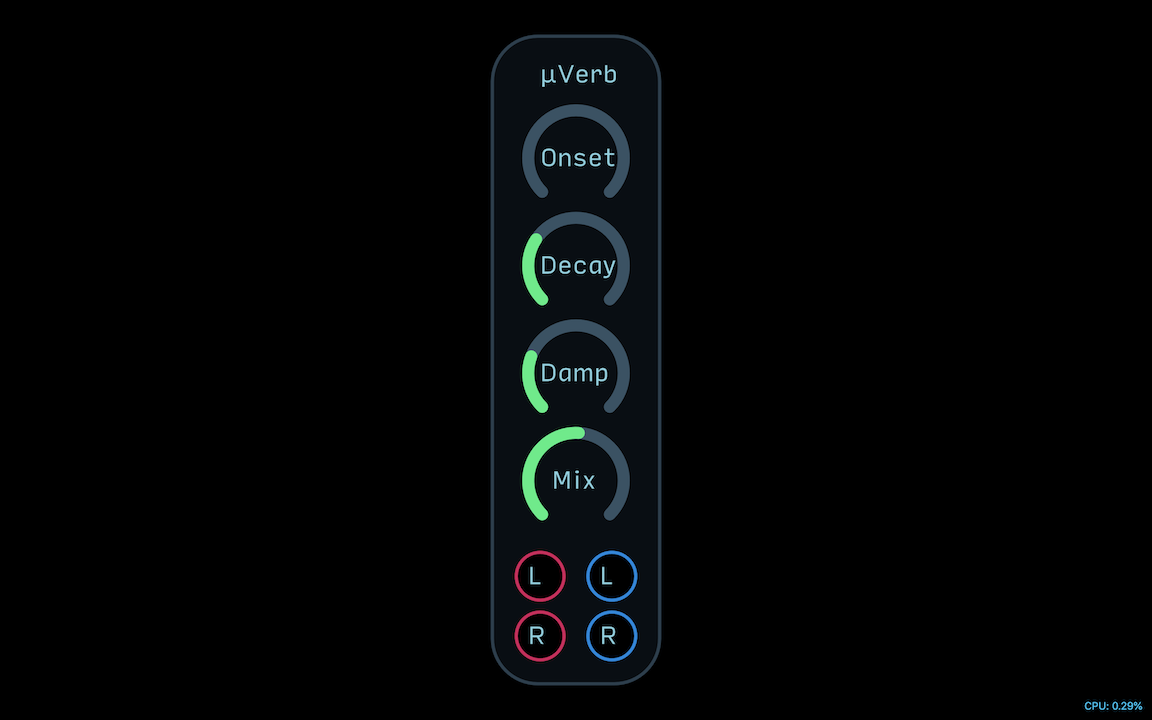
\includegraphics[width=\textwidth]{uverb.png}

\begin{table}[ht]
\small
\sffamily
\renewcommand\arraystretch{1.5}
\centering
\begin{tabular}{l*{1}{>{\raggedright\arraybackslash}p{0.7\linewidth}}}

\toprule
\textbf{Knob} \\
Onset & \textit{Pre-delay amount.} \\
Decay & \textit{Sets the decay time of the reverberations.} \\
Damp & \textit{Dampens reverberations.} \\
Mix & \textit{Adjusts the wet/dry balance.} \\

\midrule
\textbf{Input} \\
Left/Right & \textit{Stereo audio input.} \\

\midrule
\textbf{Output} \\
Left/Right & \textit{Stereo audio output.} \\

\bottomrule
\end{tabular}
\end{table}% \\

\pagebreak


\chapter{Envelope Modules}
\pagebreak

\section{Analog Envelope}

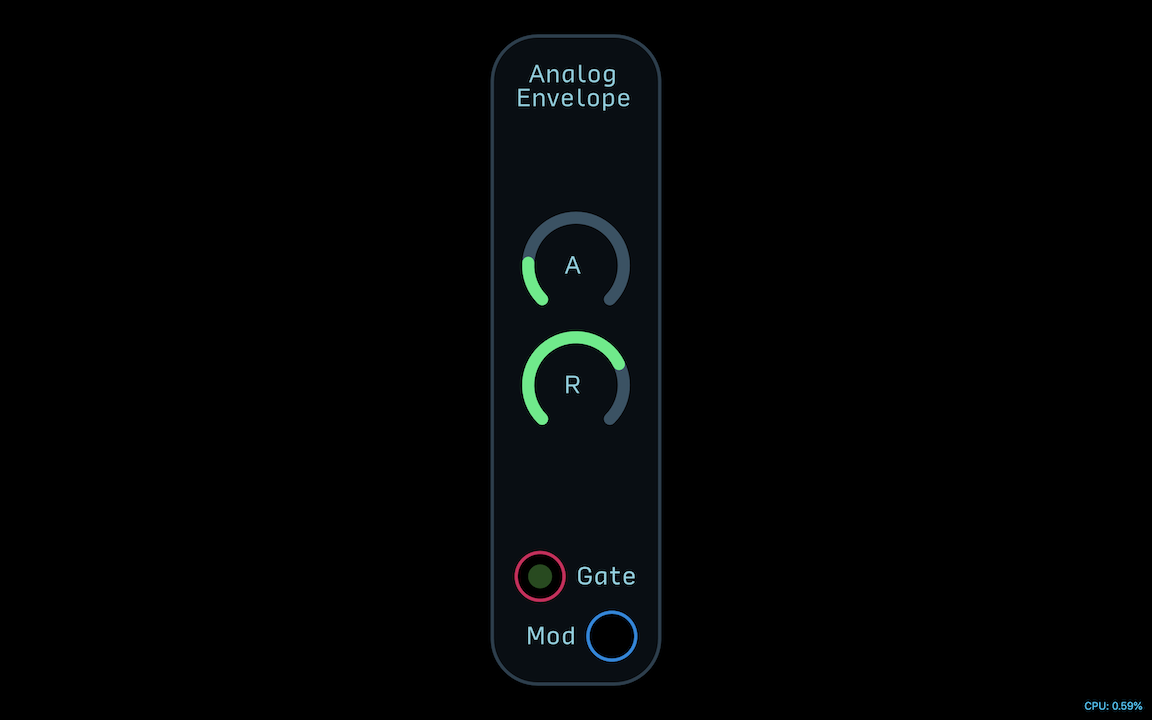
\includegraphics[width=\textwidth]{analog-envelope.png}

\begin{table}[ht]
\small
\sffamily
\renewcommand\arraystretch{1.5}
\centering
\begin{tabular}{l*{1}{>{\raggedright\arraybackslash}p{0.7\linewidth}}}

\toprule
\textbf{Knob} \\
A & \textit{Attack time.} \\
R & \textit{Release time.} \\

\midrule
\textbf{Input} \\
Gate & \textit{Opens envelope when gated.} \\

\midrule
\textbf{Output} \\
Mod & \textit{Envelope output.} \\

\bottomrule
\end{tabular}
\end{table}% \\

\pagebreak


\section{EOC Max ADSR}

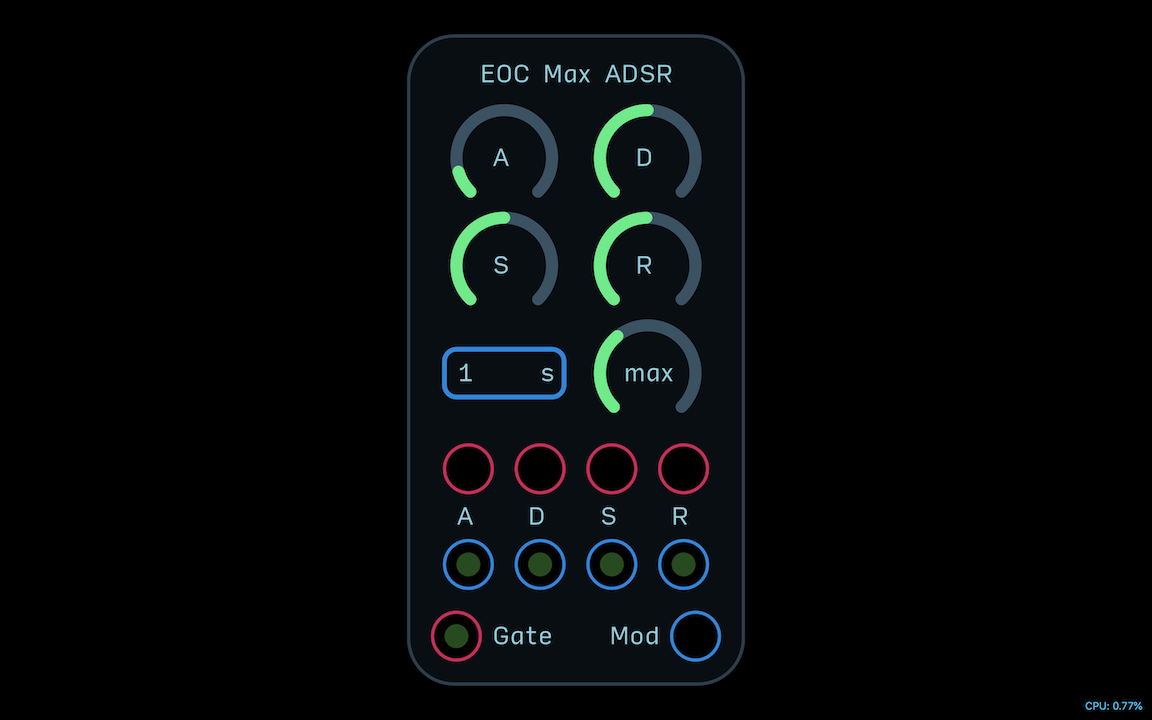
\includegraphics[width=\textwidth]{eoc-max-adsr.png}

\begin{table}[ht]
\small
\sffamily
\renewcommand\arraystretch{1.5}
\centering
\begin{tabular}{l*{1}{>{\raggedright\arraybackslash}p{0.7\linewidth}}}

\toprule
\textbf{Knob} \\
A & \textit{Attack time.} \\
D & \textit{Decay time.} \\
S & \textit{Sustain level.} \\
R & \textit{Release time.} \\
Max & \textit{Controls maximum time for Attack, Decay, and Release simultaneously.} \\

\midrule
\textbf{Input} \\
A/D/S/R & \textit{Modulation inputs for Attack, Decay, Sustain, and Release parameters.} \\
Gate & \textit{Opens envelope when gated.} \\

\midrule
\textbf{Output} \\
A/D/S/R & \textit{Gate outputs that go high at the beginning of each stage.} \\
Mod & \textit{Envelope output.} \\

\bottomrule
\end{tabular}
\end{table}% \\

\pagebreak


\section{$\mu$ADSR}

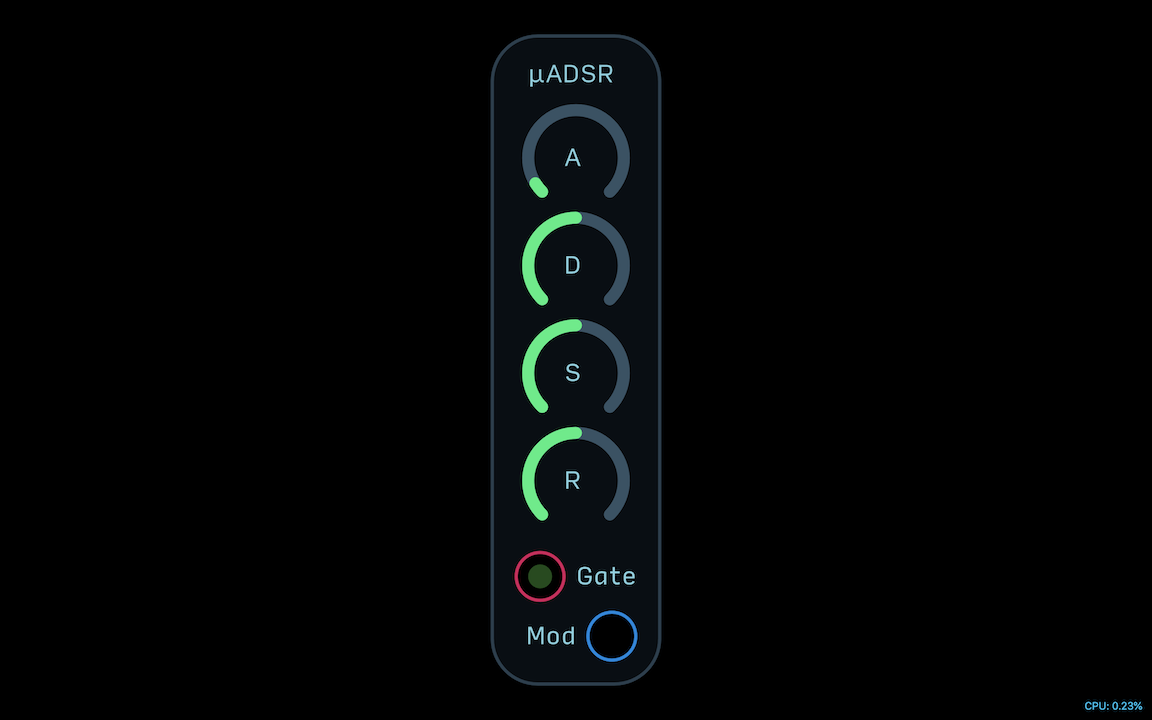
\includegraphics[width=\textwidth]{uadsr.png}

\begin{table}[ht]
\small
\sffamily
\renewcommand\arraystretch{1.5}
\centering
\begin{tabular}{l*{1}{>{\raggedright\arraybackslash}p{0.7\linewidth}}}

\toprule
\textbf{Knob} \\
A & \textit{Attack time.} \\
D & \textit{Decay time.} \\
S & \textit{Sustain level.} \\
R & \textit{Release time.} \\

\midrule
\textbf{Input} \\
Gate & \textit{Opens envelope when gated.} \\

\midrule
\textbf{Output} \\
Mod & \textit{Envelope output.} \\

\bottomrule
\end{tabular}
\end{table}% \\

\pagebreak


\chapter{Input-Output Modules}
\pagebreak

\section{Audio Input}

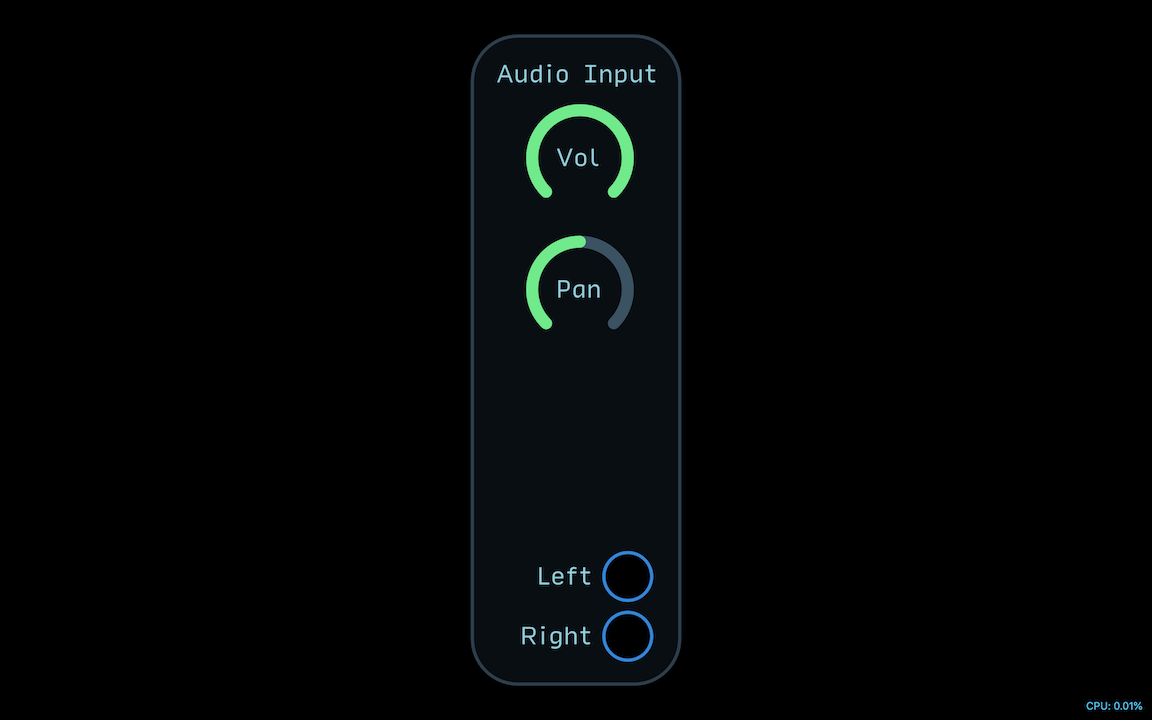
\includegraphics[width=\textwidth]{audio-input.png}

\begin{table}[ht]
\small
\sffamily
\renewcommand\arraystretch{1.5}
\centering
\begin{tabular}{l*{1}{>{\raggedright\arraybackslash}p{0.7\linewidth}}}

\toprule
\textbf{Knob} \\
Vol & \textit{Audio input volume.} \\
Pan & \textit{Audio input pan.} \\

\midrule
\textbf{Input} \\
Left/Right & \textit{Stereo audio input from channels 1 and 2 (can change channels within module).} \\

\bottomrule
\end{tabular}
\end{table}% \\

\pagebreak


\section{Audio Output}

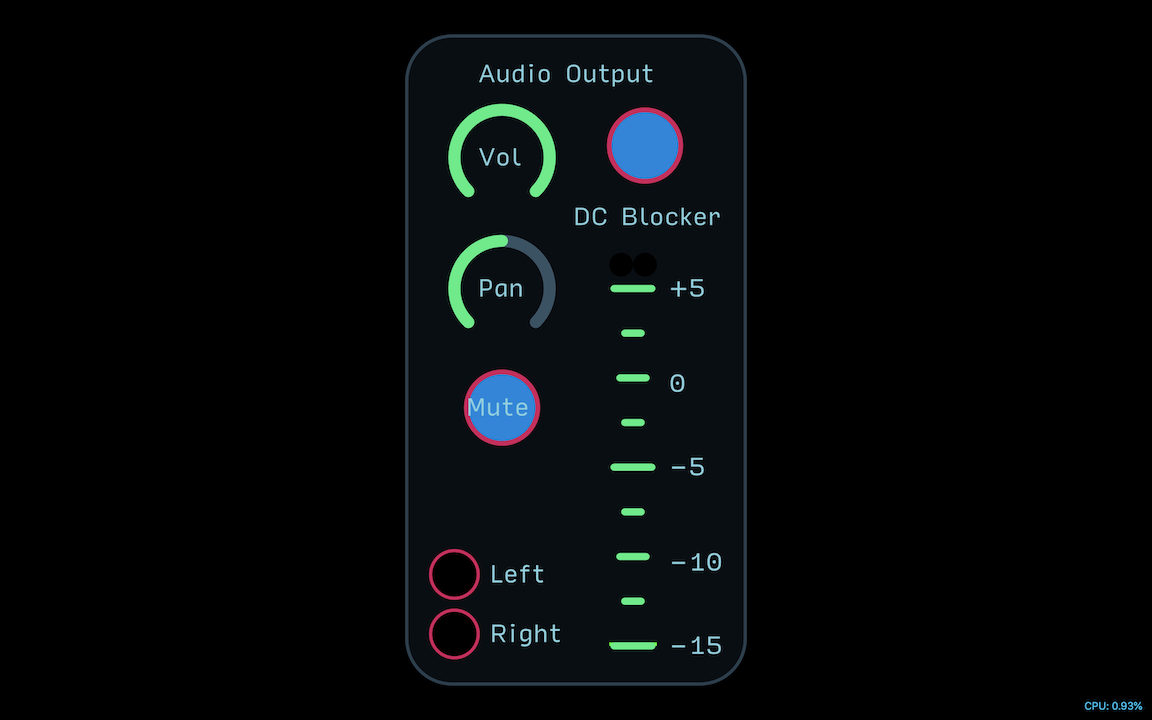
\includegraphics[width=\textwidth]{audio-output.png}

\begin{table}[ht]
\small
\sffamily
\renewcommand\arraystretch{1.5}
\centering
\begin{tabular}{l*{1}{>{\raggedright\arraybackslash}p{0.7\linewidth}}}

\toprule
\textbf{Knob} \\
Vol & \textit{Audio output volume.} \\
Pan & \textit{Audio output pan.} \\

\midrule
\textbf{Button} \\
DC Blocker & \textit{AC-couples output to block any DC offsets.} \\
Mute & \textit{Mutes audio output.} \\

\midrule
\textbf{Output} \\
Left/Right & \textit{Stereo audio output to channels 1 and 2 (can change channels within module).} \\

\bottomrule
\end{tabular}
\end{table}% \\

\pagebreak


\section{Expert Sleepers ES-3}

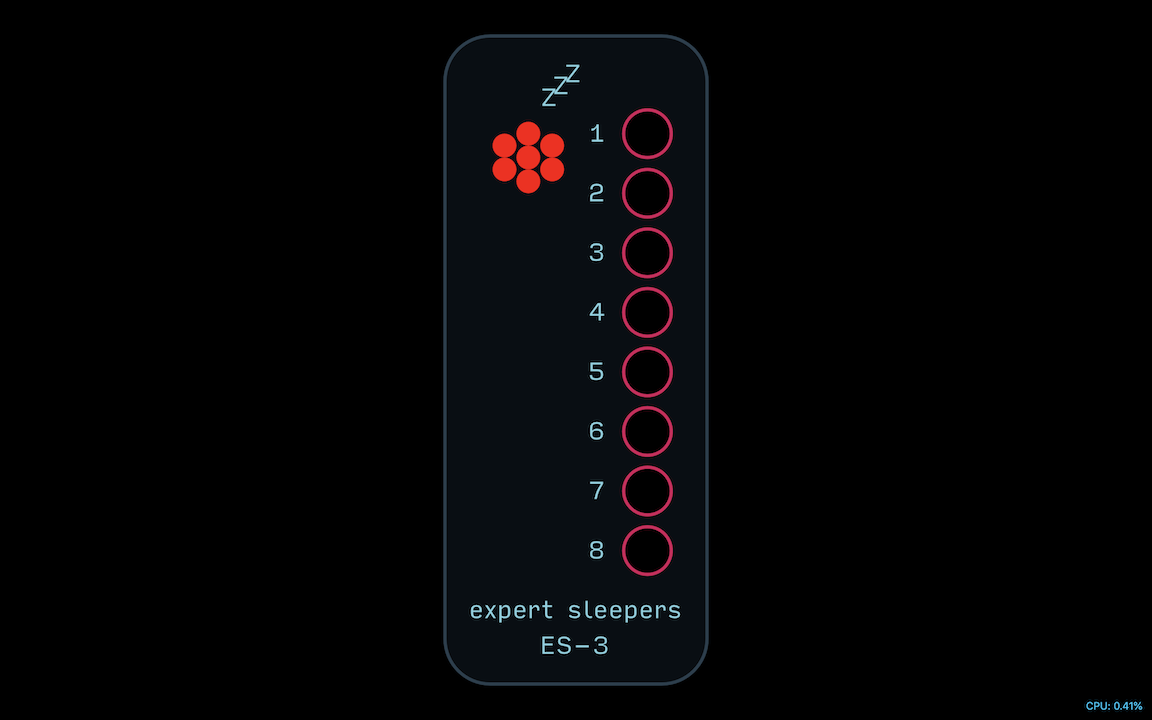
\includegraphics[width=\textwidth]{expert-sleepers-es-3.png}

\begin{table}[ht]
\small
\sffamily
\renewcommand\arraystretch{1.5}
\centering
\begin{tabular}{l*{1}{>{\raggedright\arraybackslash}p{0.7\linewidth}}}

\toprule
\textbf{Output} \\
1-8 & \textit{The 8 outputs that correspond to the 8 inputs of the Expert Sleepers ES-3} \\

\bottomrule
\end{tabular}
\end{table}% \\

\pagebreak


\section{Expert Sleepers ES-6}

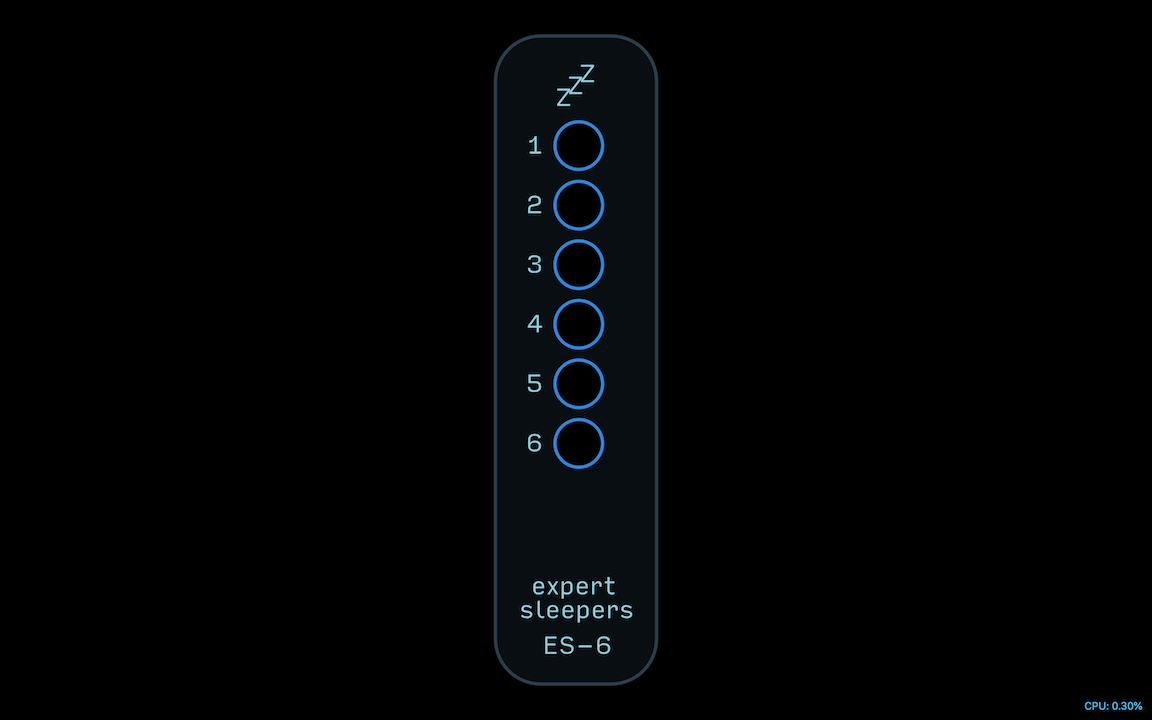
\includegraphics[width=\textwidth]{expert-sleepers-es-6.png}

\begin{table}[ht]
\small
\sffamily
\renewcommand\arraystretch{1.5}
\centering
\begin{tabular}{l*{1}{>{\raggedright\arraybackslash}p{0.7\linewidth}}}

\toprule
\textbf{Input} \\
1-6 & \textit{The 6 inputs that correspond to the 6 outputs of the Expert Sleepers ES-6.} \\

\bottomrule
\end{tabular}
\end{table}% \\

\pagebreak


\section{Expert Sleepers ES-8}

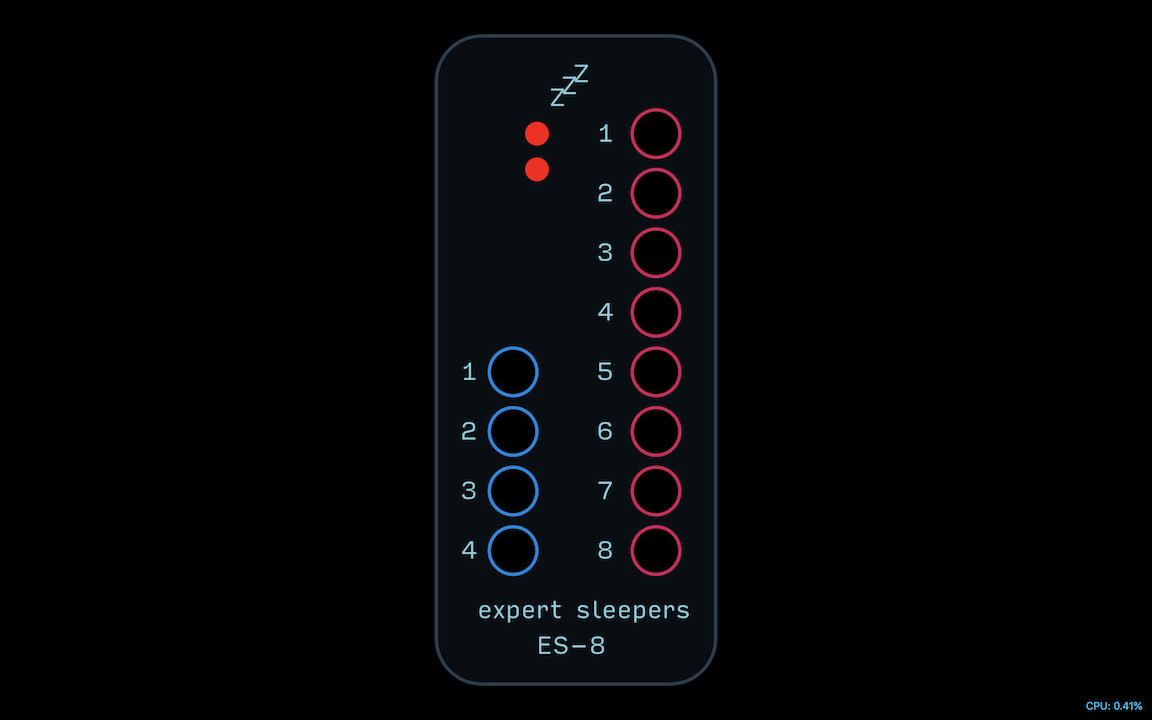
\includegraphics[width=\textwidth]{expert-sleepers-es-8.png}

\begin{table}[ht]
\small
\sffamily
\renewcommand\arraystretch{1.5}
\centering
\begin{tabular}{l*{1}{>{\raggedright\arraybackslash}p{0.7\linewidth}}}

\toprule
\textbf{Input} \\
1-4 & \textit{The 4 inputs that correspond to the 4 outputs of the Expert Sleepers ES-8.} \\

\midrule
\textbf{Output} \\
1-6 & \textit{The 8 outputs that correspond to the 8 inputs of the Expert Sleepers ES-8.} \\

\bottomrule
\end{tabular}
\end{table}% \\

\pagebreak


\section{MIDI Input}

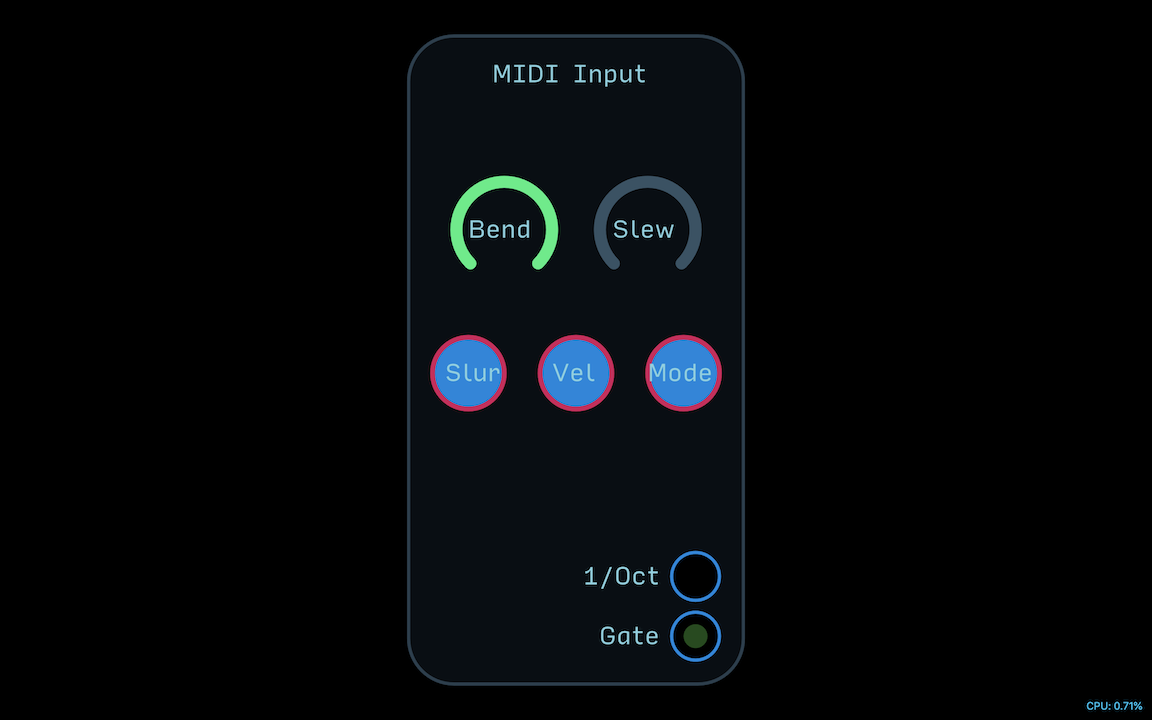
\includegraphics[width=\textwidth]{midi-input.png}

\begin{table}[ht]
\small
\sffamily
\renewcommand\arraystretch{1.5}
\centering
\begin{tabular}{l*{1}{>{\raggedright\arraybackslash}p{0.7\linewidth}}}

\toprule
\textbf{Knob} \\
Bend & \textit{Adjusts the range of the pitch bend wheel.} \\
Slew & \textit{Adjusts the amount of slew between notes.} \\

\midrule
\textbf{Button} \\
Slur & \textit{When engaged, will not retrigger gate if notes overlap in monophonic mode.} \\
Vel & \textit{When engaged, will allow velocity of notes to affect gate height.} \\
Mode & \textit{Switches between two slew modes: off = equal time (digital); on = longer slew between notes further apart (analog).} \\

\midrule
\textbf{Output} \\
1/Oct & \textit{1/Octave output.} \\
Gate & \textit{Gate output.} \\

\bottomrule
\end{tabular}
\end{table}% \\

\pagebreak


\section{VPO Converter}

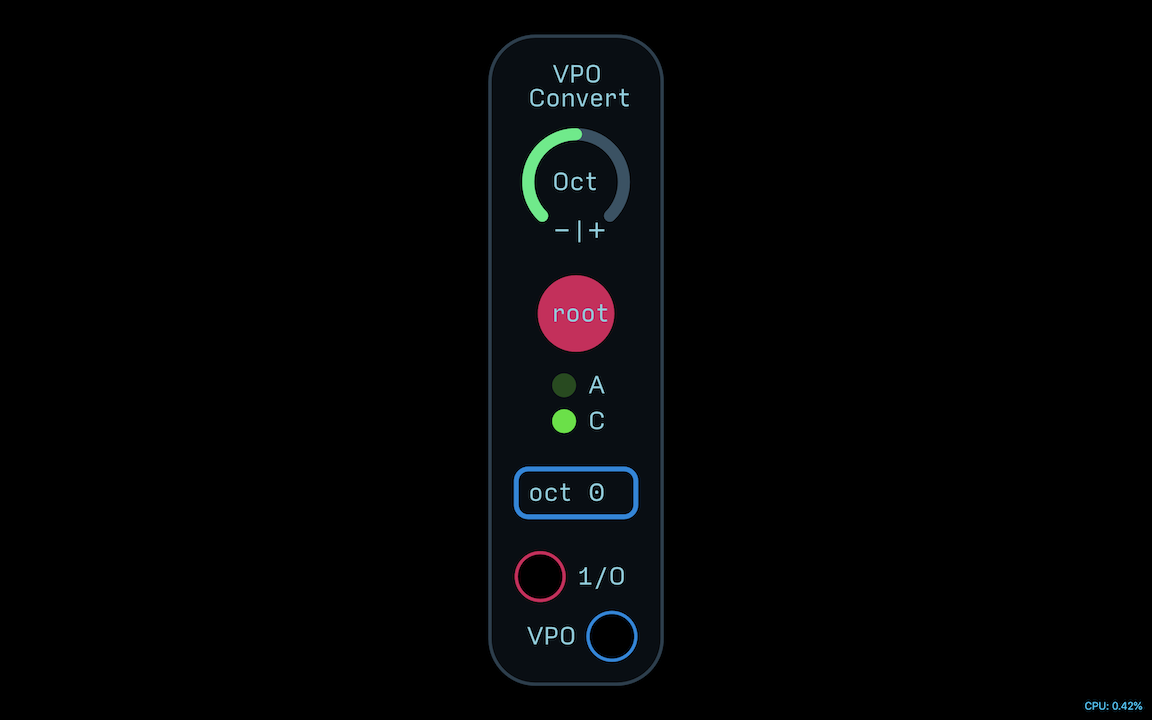
\includegraphics[width=\textwidth]{vpo-converter.png}

\begin{table}[ht]
\small
\sffamily
\renewcommand\arraystretch{1.5}
\centering
\begin{tabular}{l*{1}{>{\raggedright\arraybackslash}p{0.7\linewidth}}}

\toprule
\textbf{Knob} \\
Oct & \textit{Shifts input 1/Octave signal up and down by octaves.} \\

\midrule
\textbf{Button} \\
Root & \textit{Sets the lowest note to either A or C.} \\

\midrule
\textbf{Input} \\
1/O & \textit{1/Octave input.} \\

\midrule
\textbf{Output} \\
VPO & \textit{Volt per octave output. Scaled to connect to Expert Sleepers ES-3 and ES-8 or any DC-Coupled audio interface with a voltage swing of +/- 10 volts.} \\

\bottomrule
\end{tabular}
\end{table}% \\

\pagebreak


\chapter{LFO Modules}
\pagebreak

\section{Basic LFO}

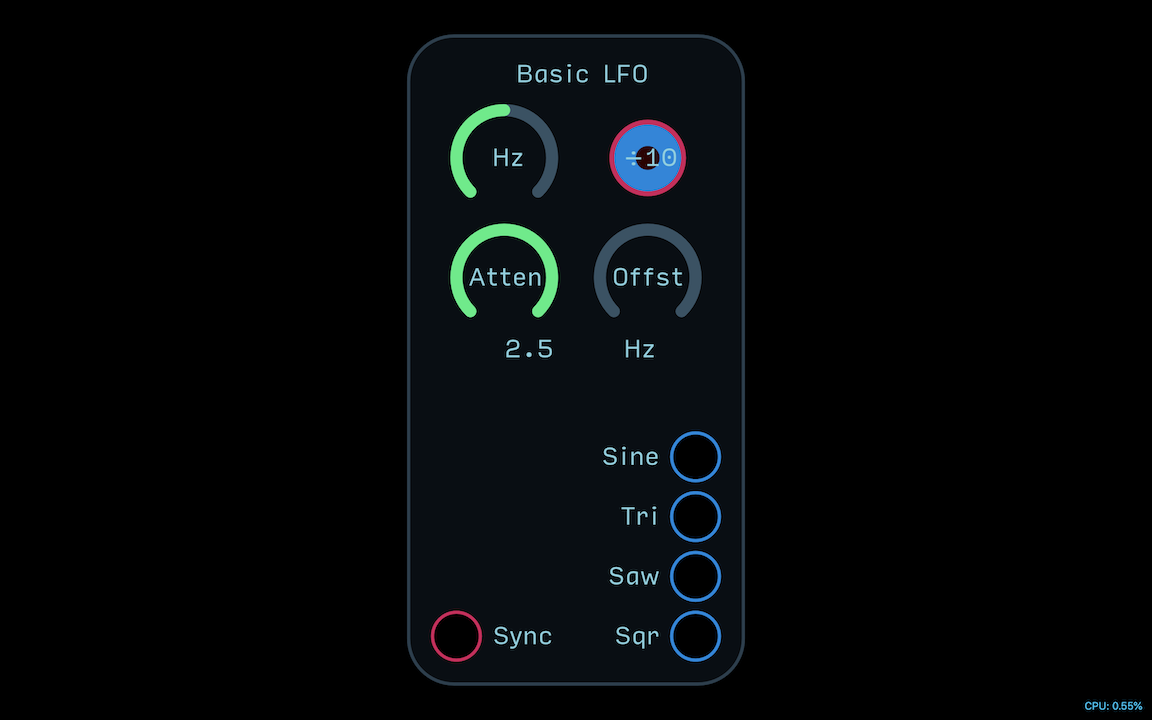
\includegraphics[width=\textwidth]{basic-lfo.png}

\begin{table}[ht]
\small
\sffamily
\renewcommand\arraystretch{1.5}
\centering
\begin{tabular}{l*{1}{>{\raggedright\arraybackslash}p{0.7\linewidth}}}

\toprule
\textbf{Knob} \\
Hz & \textit{Speed of the LFO from 0 to 20Hz, or 0 to 2Hz when $\div$10 button is engaged.} \\
Atten & \textit{Attenuates LFO signal.} \\
Offst & \textit{Shifts LFO up or down. Note: LFO output will clip if output exceeds the 0 to 1 modulation range.} \\

\midrule
\textbf{Button} \\
$\div$10 & \textit{Divides maximum LFO speed by 10.} \\

\midrule
\textbf{Input} \\
Sync & \textit{Uses a gate, LFO, or audio signal to hard reset LFO wave.} \\

\midrule
\textbf{Output} \\
Sine/Tri/Saw/Sqr & \textit{Sine, triangle, saw, and square wave outputs.} \\

\bottomrule
\end{tabular}
\end{table}% \\

\pagebreak


\section{Octature Sine LFO}

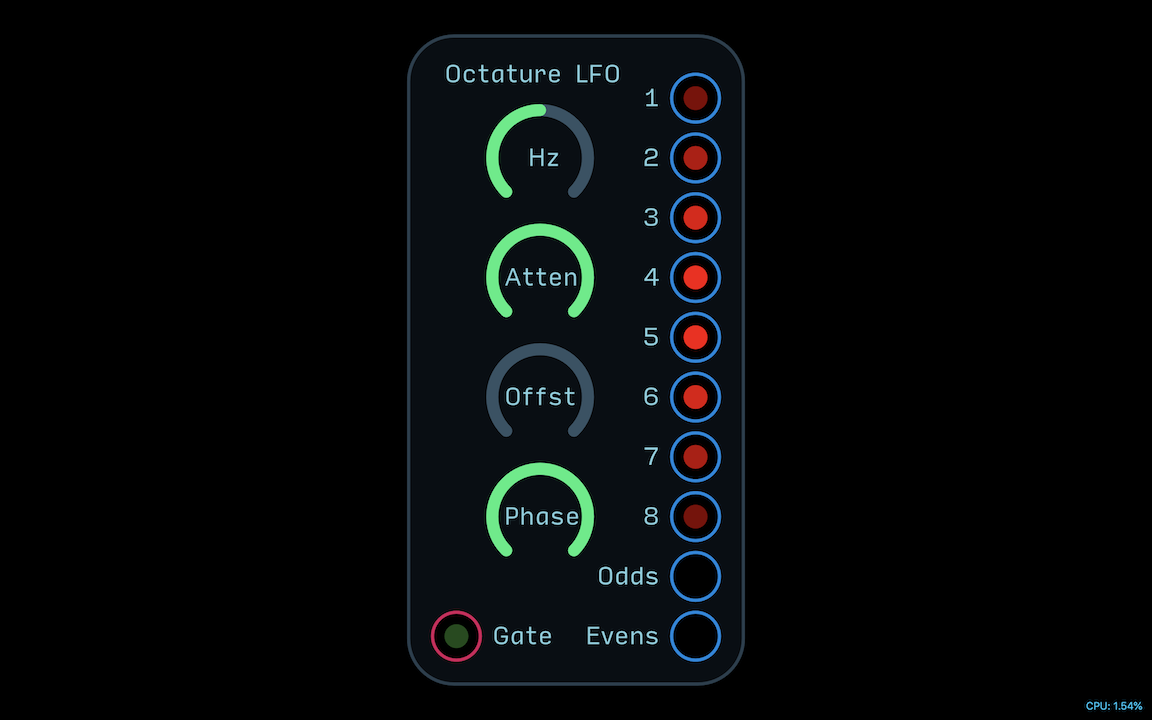
\includegraphics[width=\textwidth]{octature-sine-lfo.png}

\begin{table}[ht]
\small
\sffamily
\renewcommand\arraystretch{1.5}
\centering
\begin{tabular}{l*{1}{>{\raggedright\arraybackslash}p{0.7\linewidth}}}

\toprule
\textbf{Knob} \\
Hz & \textit{Speed of the LFO from 0 to 20Hz.} \\
Atten & \textit{Attenuates LFO signal.} \\
Offst & \textit{Shifts LFO up or down. Note: LFO output will clip if output exceeds the 0 to 1 modulation range.} \\
Phase & \textit{Adjusts the phase ratios between each output from $0\,^{\circ}$ to $22.5\,^{\circ}$.} \\

\midrule
\textbf{Input} \\
Sync & \textit{Uses a gate, LFO, or audio signal to hard reset LFO wave.} \\

\midrule
\textbf{Output} \\
1-8 & \textit{Sine LFO outputs.} \\
Odds/Evens & \textit{Groups outputs 1, 3, 5, 7 and 2, 4, 6, 8 into two quad  polyphonic signals.} \\

\bottomrule
\end{tabular}
\end{table}% \\

\pagebreak


\section{TZFM LFO}

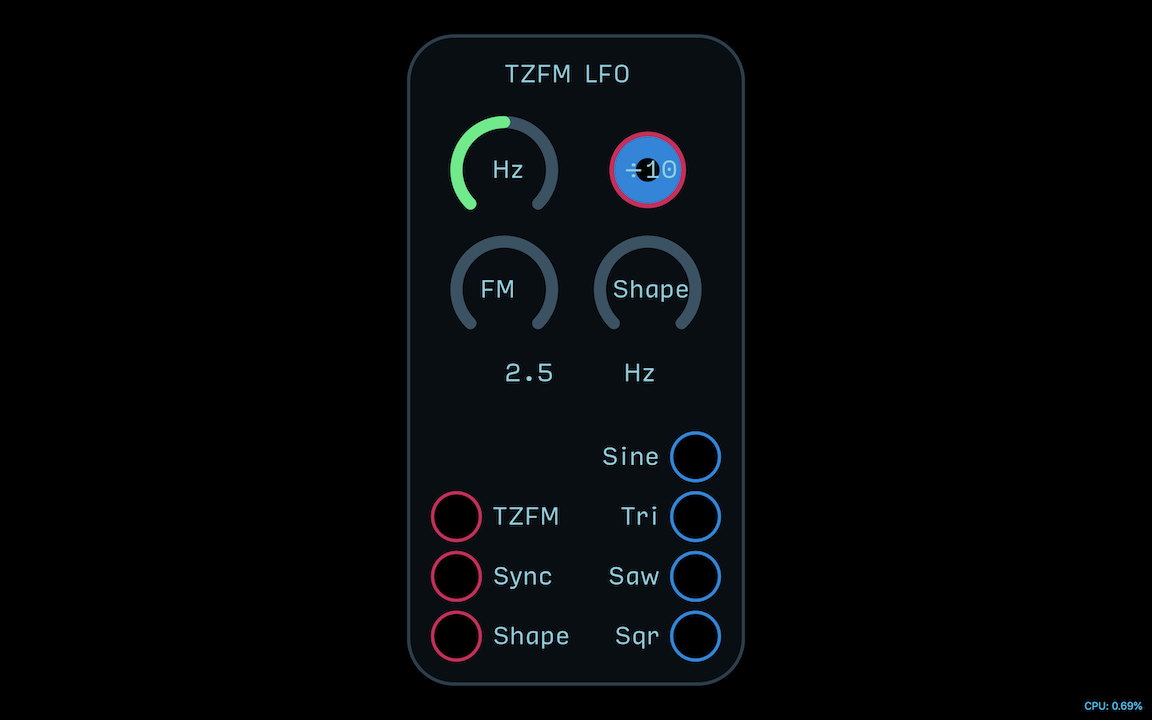
\includegraphics[width=\textwidth]{tzfm-lfo.png}

\begin{table}[ht]
\small
\sffamily
\renewcommand\arraystretch{1.5}
\centering
\begin{tabular}{l*{1}{>{\raggedright\arraybackslash}p{0.7\linewidth}}}

\toprule
\textbf{Knob} \\
Hz & \textit{Speed of the LFO from 0 to 20Hz, or 0 to 2Hz when $\div$10 button is engaged.} \\
FM & \textit{Attenuates the incoming modulation signal at the TZFM input.} \\
Shape & \textit{Attenuates the incoming modulation signal at the Shape input} \\

\midrule
\textbf{Button} \\
$\div$10 & \textit{Divides maximum LFO speed by 10.} \\

\midrule
\textbf{Input} \\
TZFM & \textit{Modulation input for frequency modulation. Expects a 0 to 1 modulation signal and internally translates it into a bipolar -1 to 1 modulation signal.} \\
Sync & \textit{Uses a gate, LFO, or audio signal to hard reset LFO wave.} \\
Shape & \textit{Modulation input for shape modulation.} \\

\midrule
\textbf{Output} \\
Sine/Tri/Saw/Sqr & \textit{Sine, triangle, saw, and square wave outputs.} \\

\bottomrule
\end{tabular}
\end{table}% \\

\pagebreak


\section{$\mu$LFO}

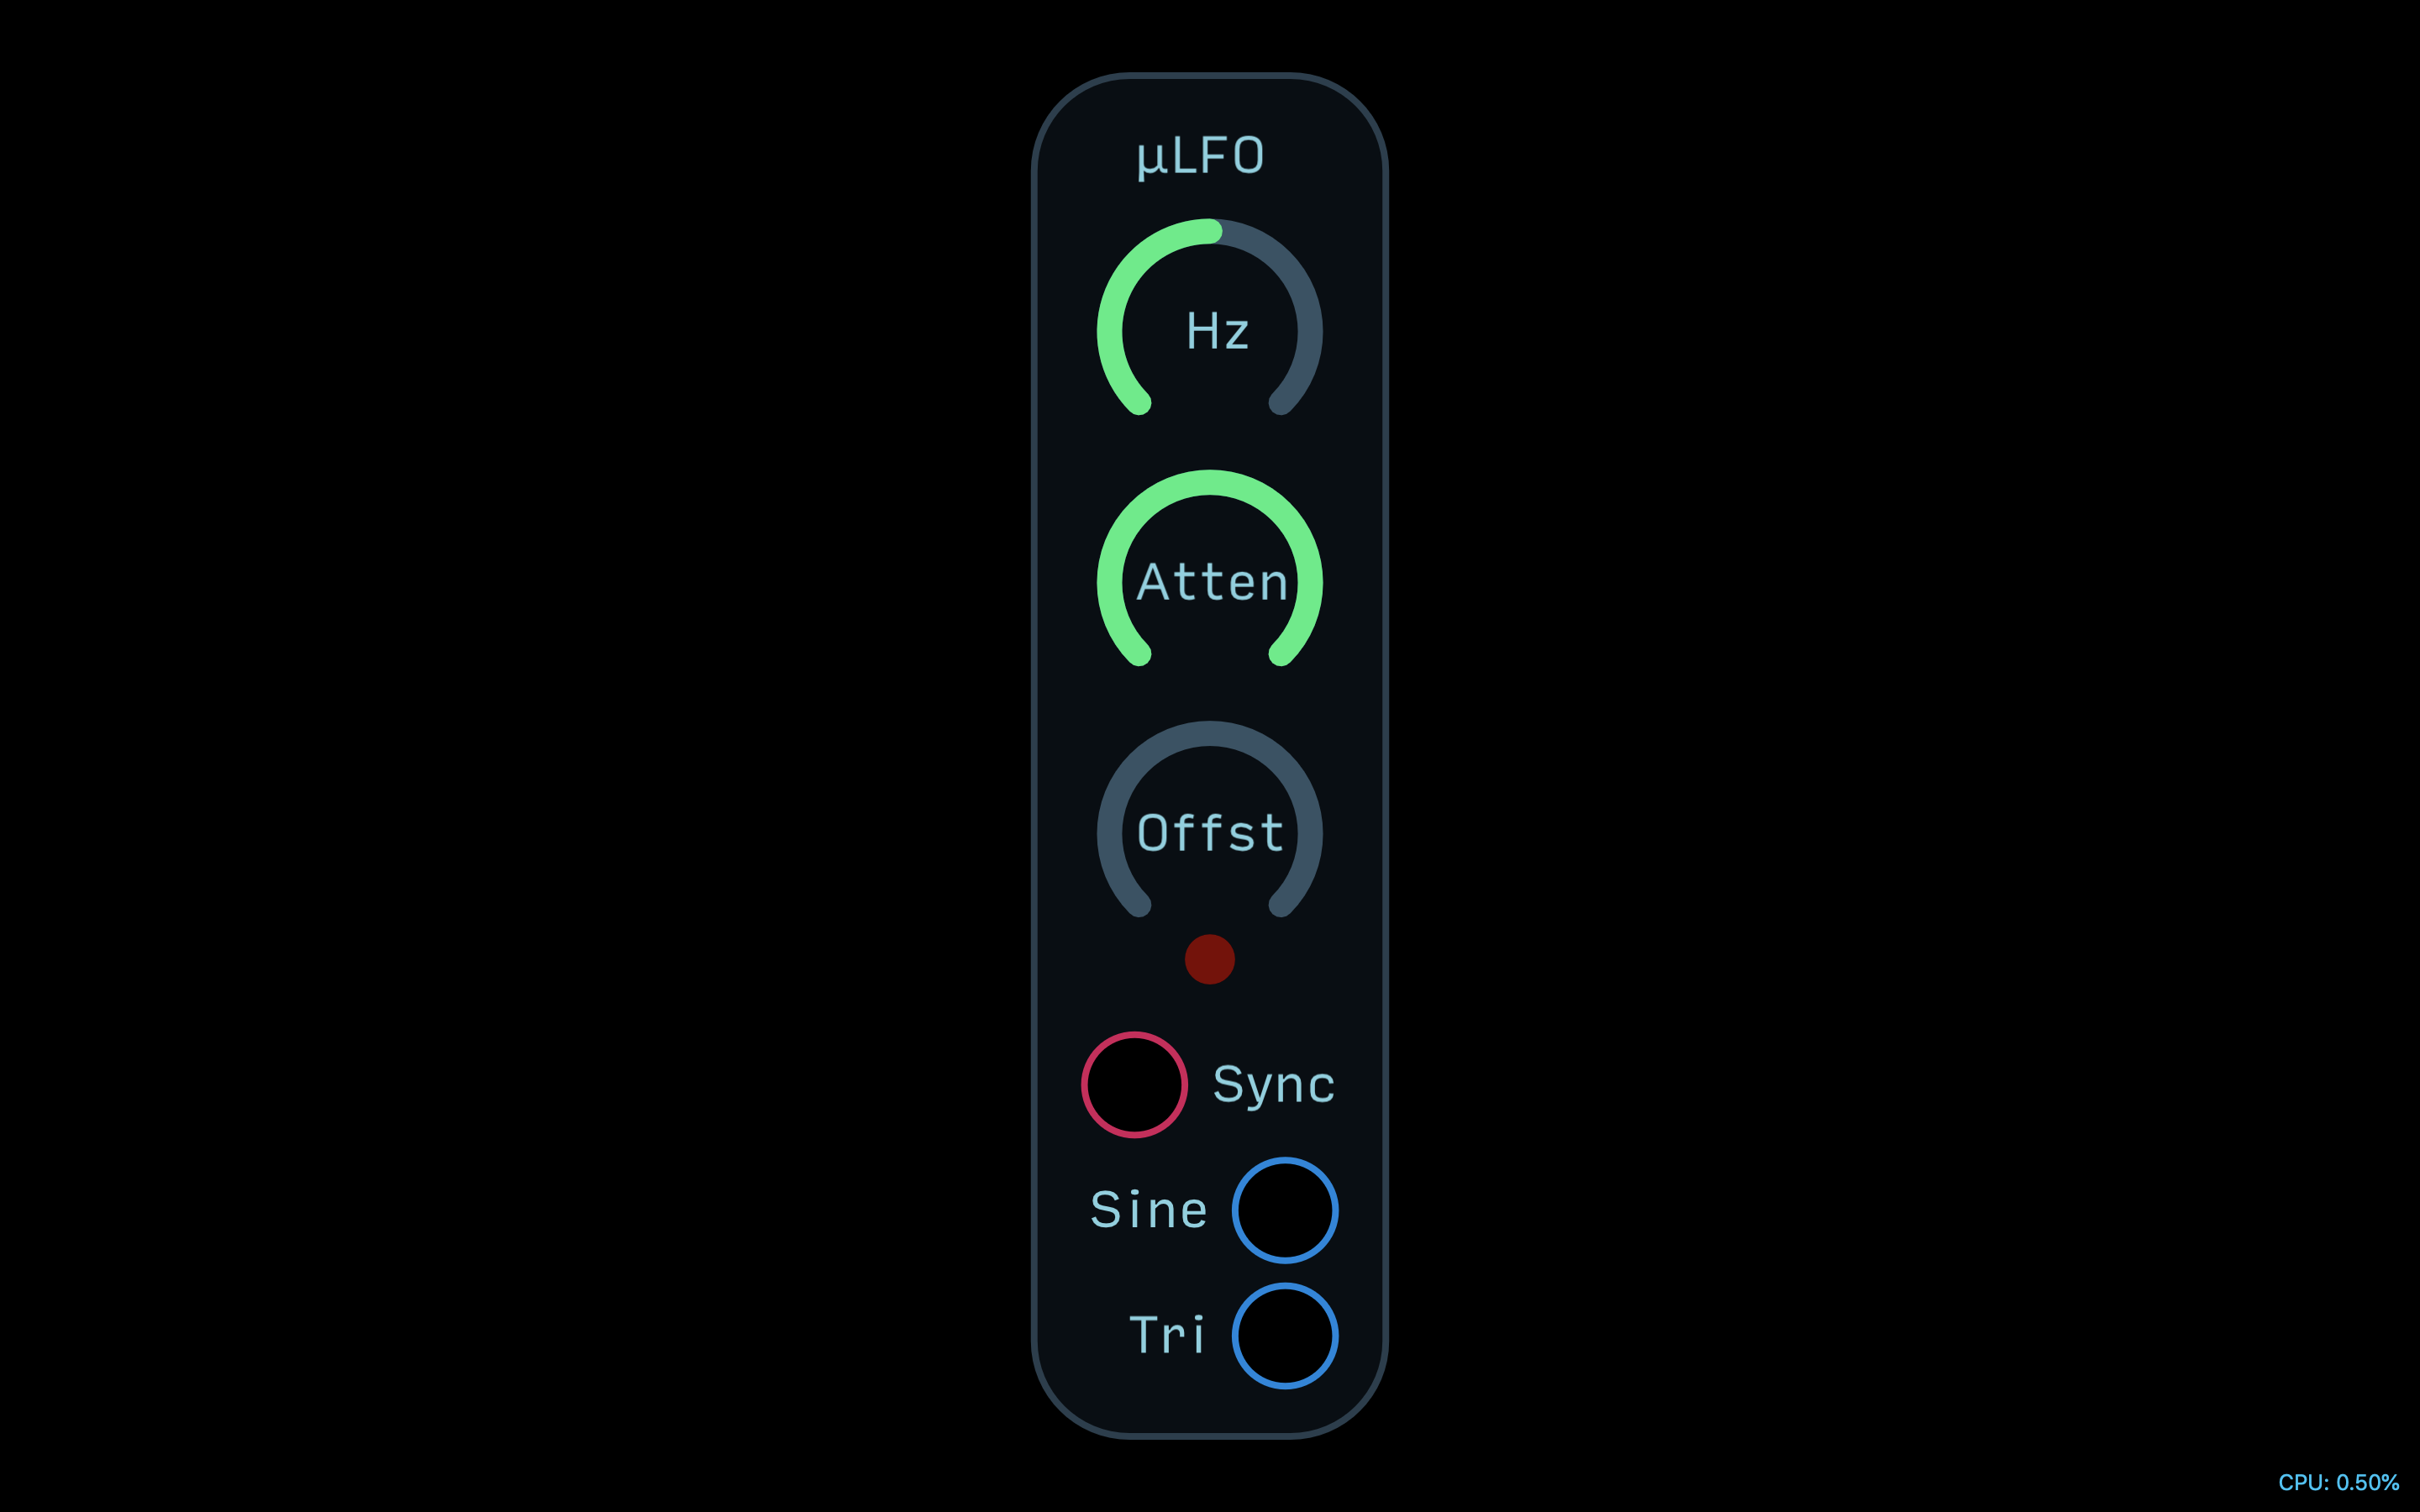
\includegraphics[width=\textwidth]{ulfo.png}

\begin{table}[ht]
\small
\sffamily
\renewcommand\arraystretch{1.5}
\centering
\begin{tabular}{l*{1}{>{\raggedright\arraybackslash}p{0.7\linewidth}}}

\toprule
\textbf{Knob} \\
Hz & \textit{Speed of the LFO from 0 to 20Hz.} \\
Atten & \textit{Attenuates LFO signal.} \\
Offst & \textit{Shifts LFO up or down. Note: LFO output will clip if output exceeds the 0 to 1 modulation range.} \\

\midrule
\textbf{Input} \\
Sync & \textit{Uses a gate, LFO, or audio signal to hard reset LFO wave.} \\

\midrule
\textbf{Output} \\
Sine/Tri & \textit{Sine and triangle wave outputs.} \\

\bottomrule
\end{tabular}
\end{table}% \\

\pagebreak


\chapter{Mixer Modules}
\pagebreak

\section{8 Channel Mixer}

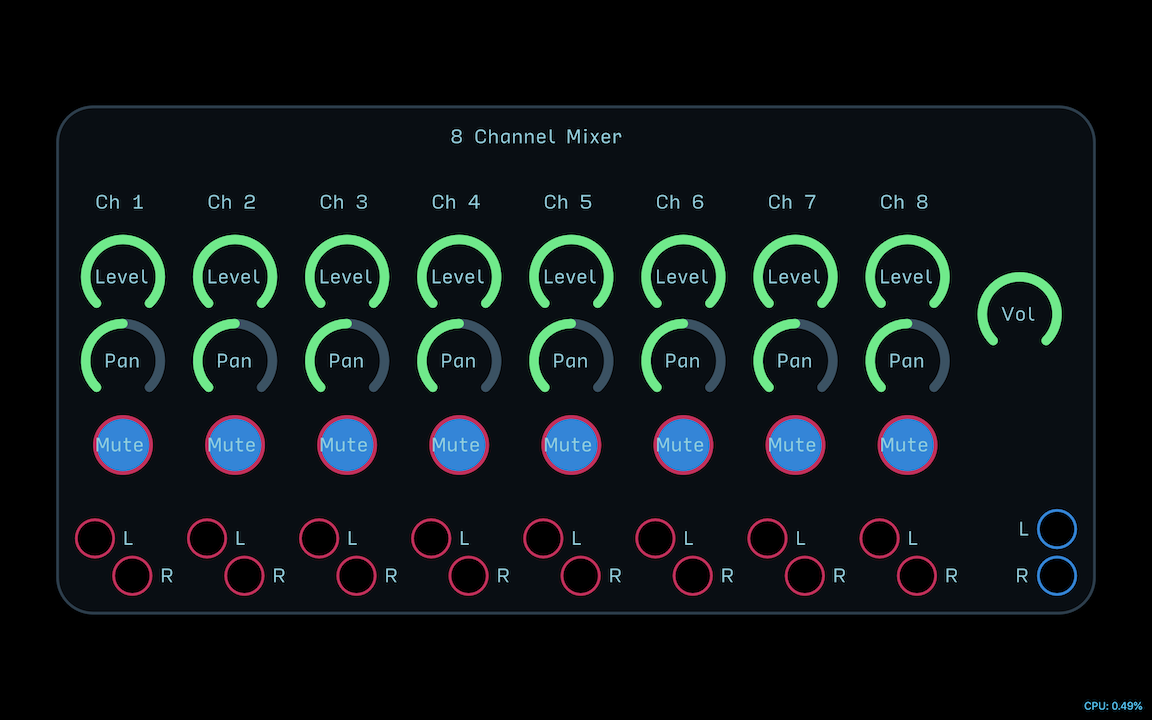
\includegraphics[width=\textwidth]{8-channel-mixer.png}

\begin{table}[ht]
\small
\sffamily
\renewcommand\arraystretch{1.5}
\centering
\begin{tabular}{l*{1}{>{\raggedright\arraybackslash}p{0.7\linewidth}}}

\toprule
\textbf{Knob} \\
Level & \textit{Adjusts the volume of the channel.} \\
Pan & \textit{Adjusts the pan of the channel} \\
Vol & \textit{Master volume for module.} \\

\midrule
\textbf{Button} \\
Mute & \textit{Mutes the channel. Has internal envelope that prevents clicking when muting.} \\

\midrule
\textbf{Input} \\
L/R & \textit{Left/Right stereo inputs for each channel.} \\

\midrule
\textbf{Output} \\
L/R & \textit{Left/Right stereo outputs.} \\

\bottomrule
\end{tabular}
\end{table}% \\

\pagebreak


\section{CV Mixer}

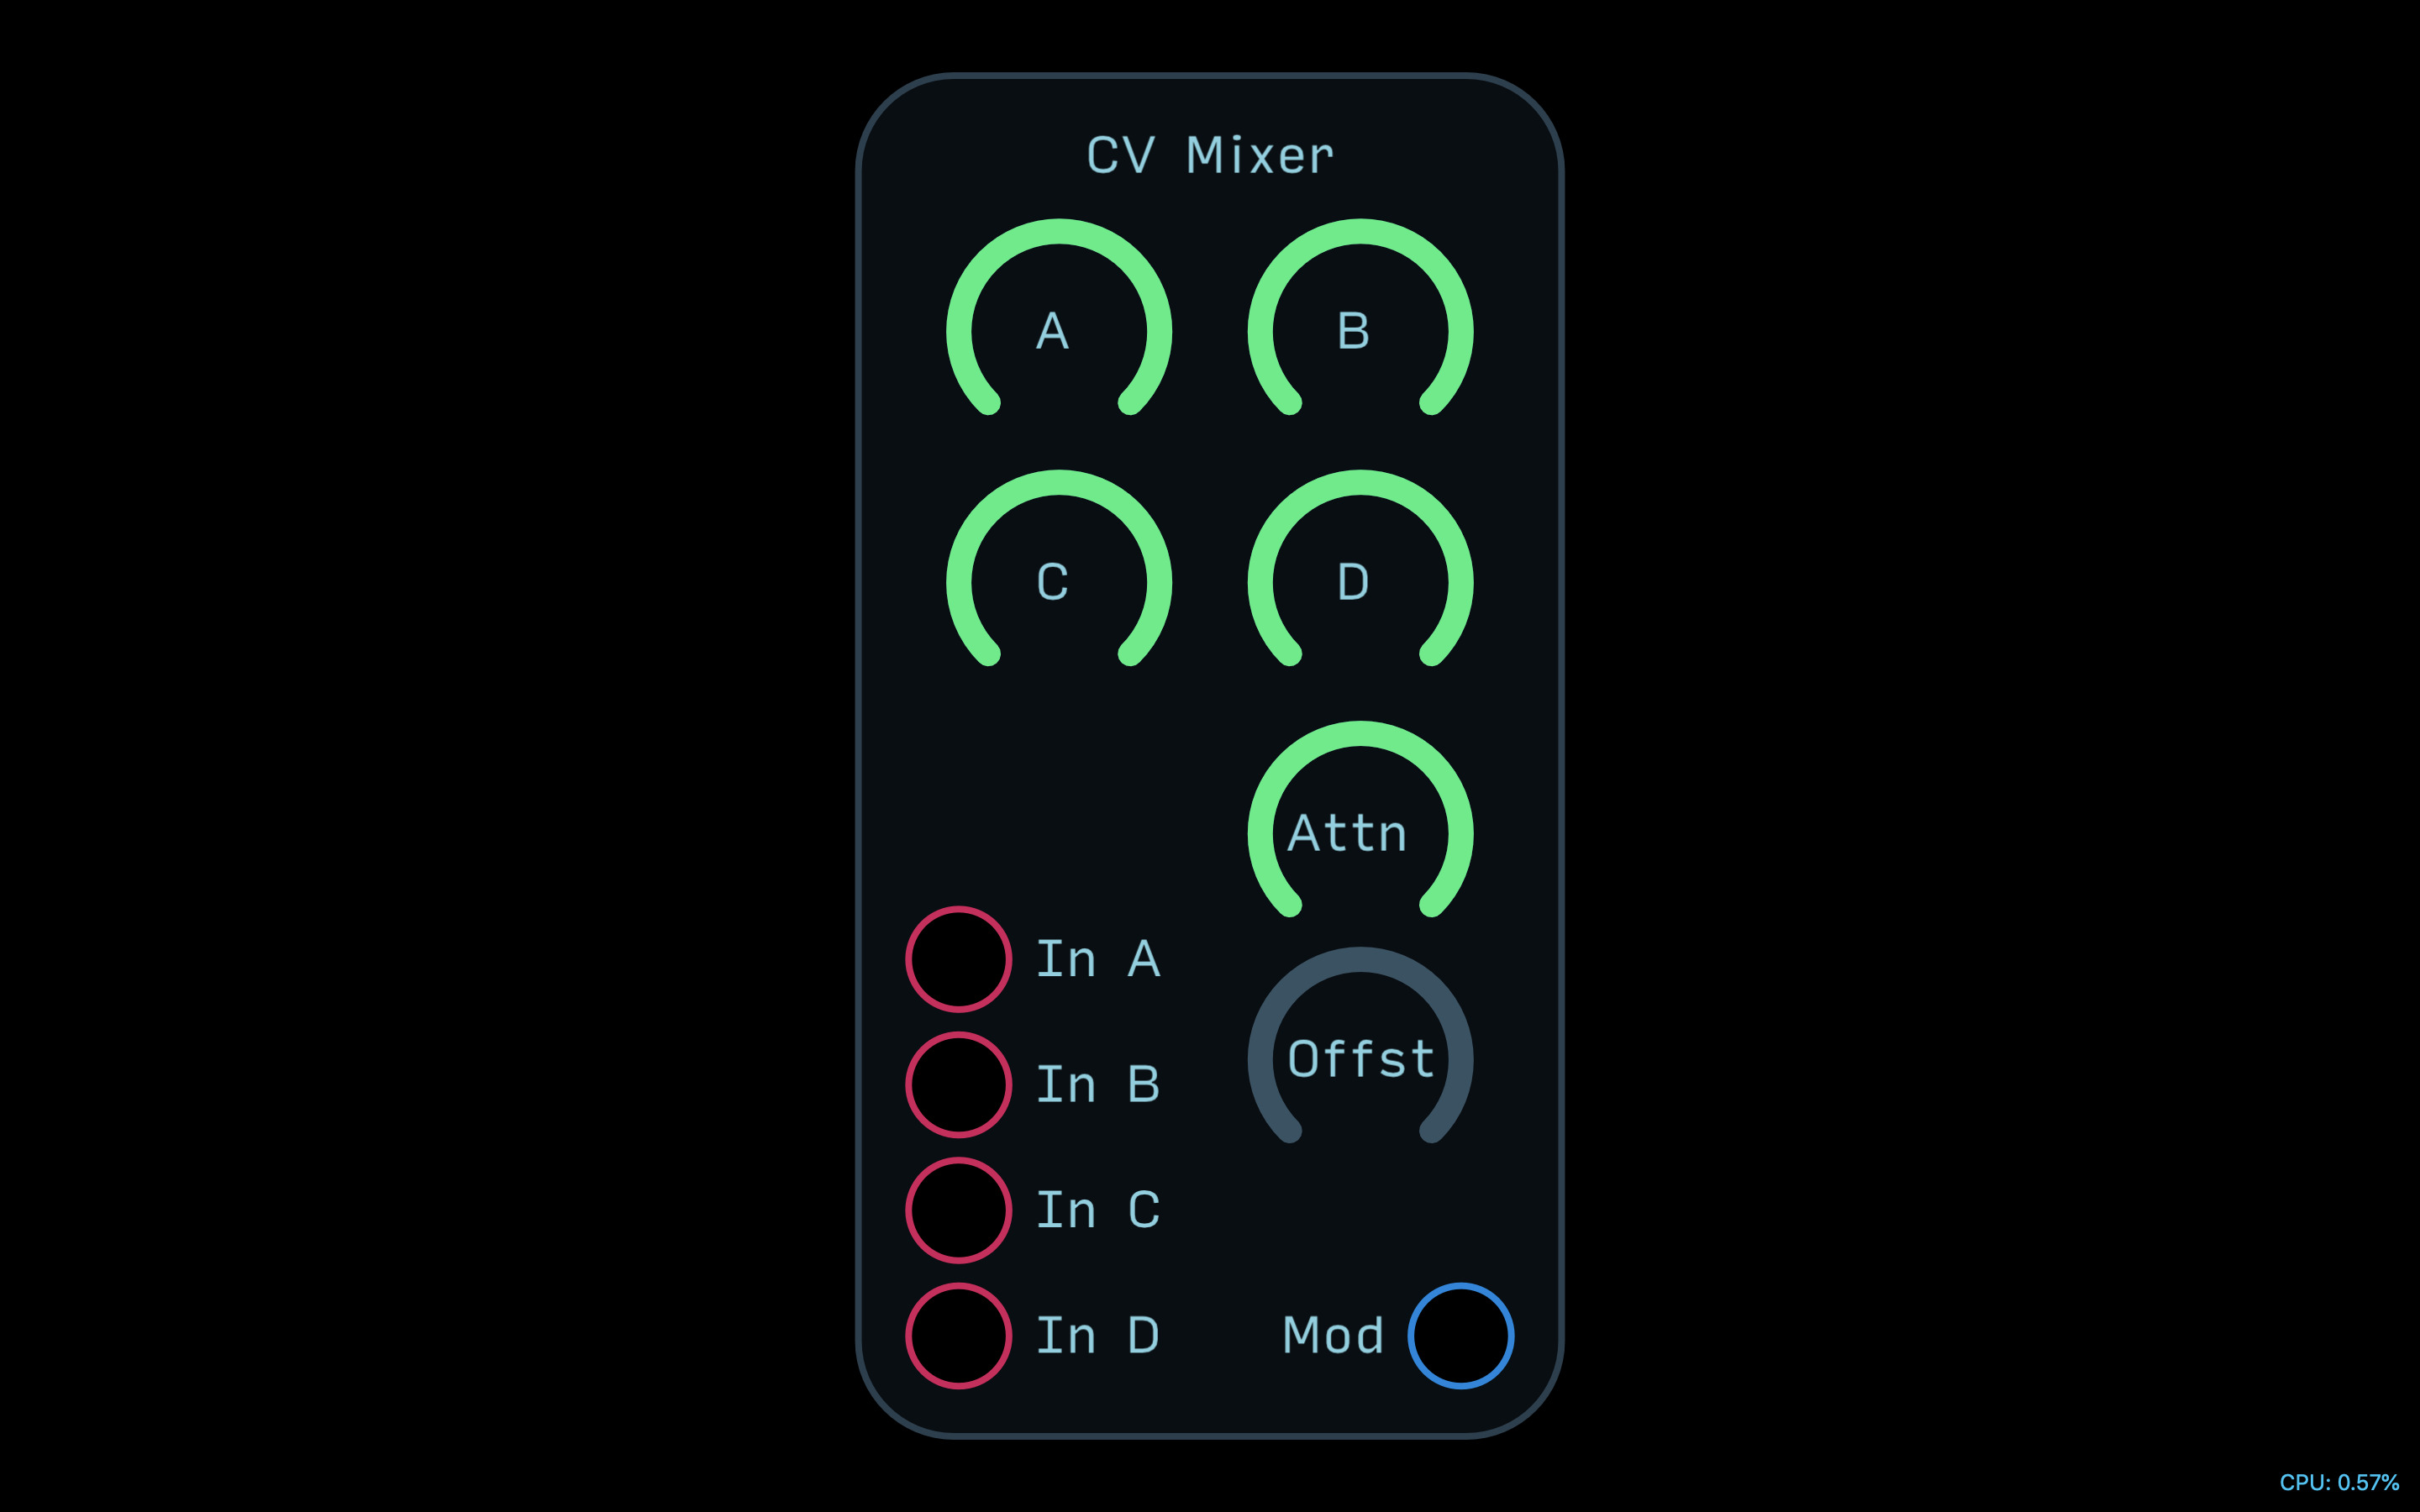
\includegraphics[width=\textwidth]{cv-mixer.png}

\begin{table}[ht]
\small
\sffamily
\renewcommand\arraystretch{1.5}
\centering
\begin{tabular}{l*{1}{>{\raggedright\arraybackslash}p{0.7\linewidth}}}

\toprule
\textbf{Knob} \\
A/B/C/D & \textit{Adjusts the level of corresponding modulation inputs.} \\
Atten & \textit{Attenuates overall modulation signal.} \\
Offst & \textit{Shifts modulation signal up or down. Note: Modulation output will clip if output exceeds the 0 to 1 modulation range.} \\

\midrule
\textbf{Input} \\
In A/B/C/D & \textit{Modulation inputs.} \\

\midrule
\textbf{Output} \\
Mod & \textit{Mixed modulation output.} \\

\bottomrule
\end{tabular}
\end{table}% \\

\pagebreak


\section{$\mu$Mix Audio}

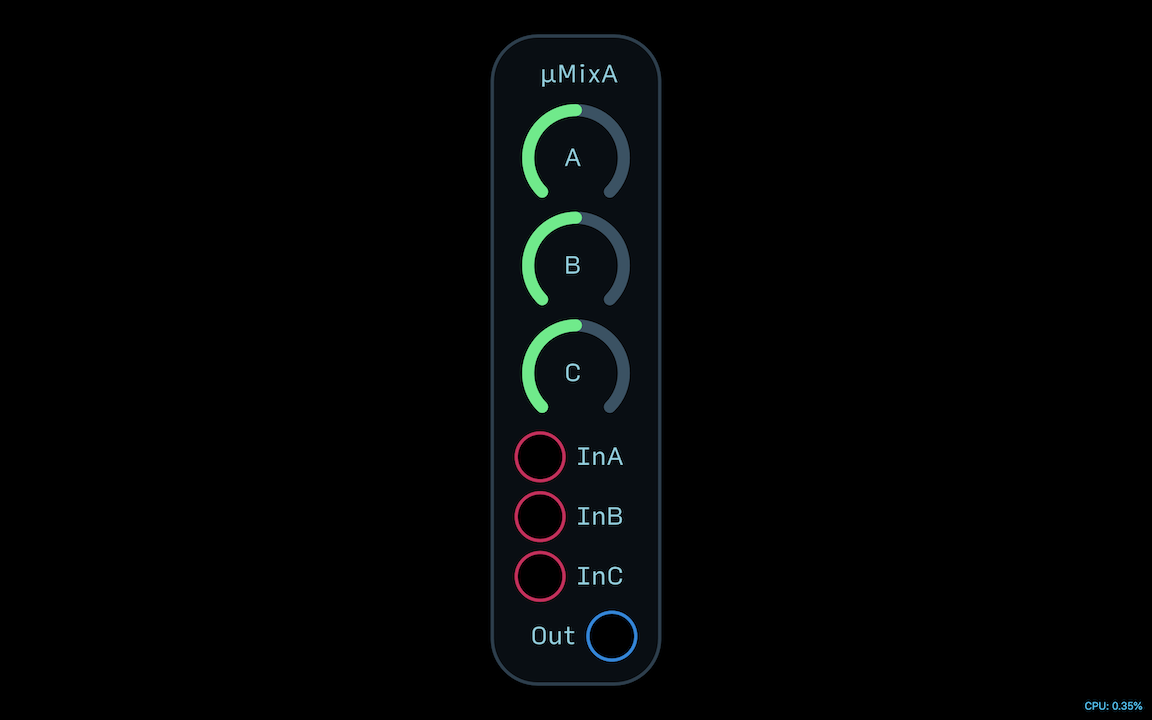
\includegraphics[width=\textwidth]{umix-audio.png}

\begin{table}[ht]
\small
\sffamily
\renewcommand\arraystretch{1.5}
\centering
\begin{tabular}{l*{1}{>{\raggedright\arraybackslash}p{0.7\linewidth}}}

\toprule
\textbf{Knob} \\
In A/B/C & \textit{Audio input attenuators.} \\

\midrule
\textbf{Input} \\
In A/B/C & \textit{Audio inputs.} \\

\midrule
\textbf{Output} \\
Out & \textit{Mixed audio output.} \\

\bottomrule
\end{tabular}
\end{table}% \\

\pagebreak


\section{$\mu$Mix CV}

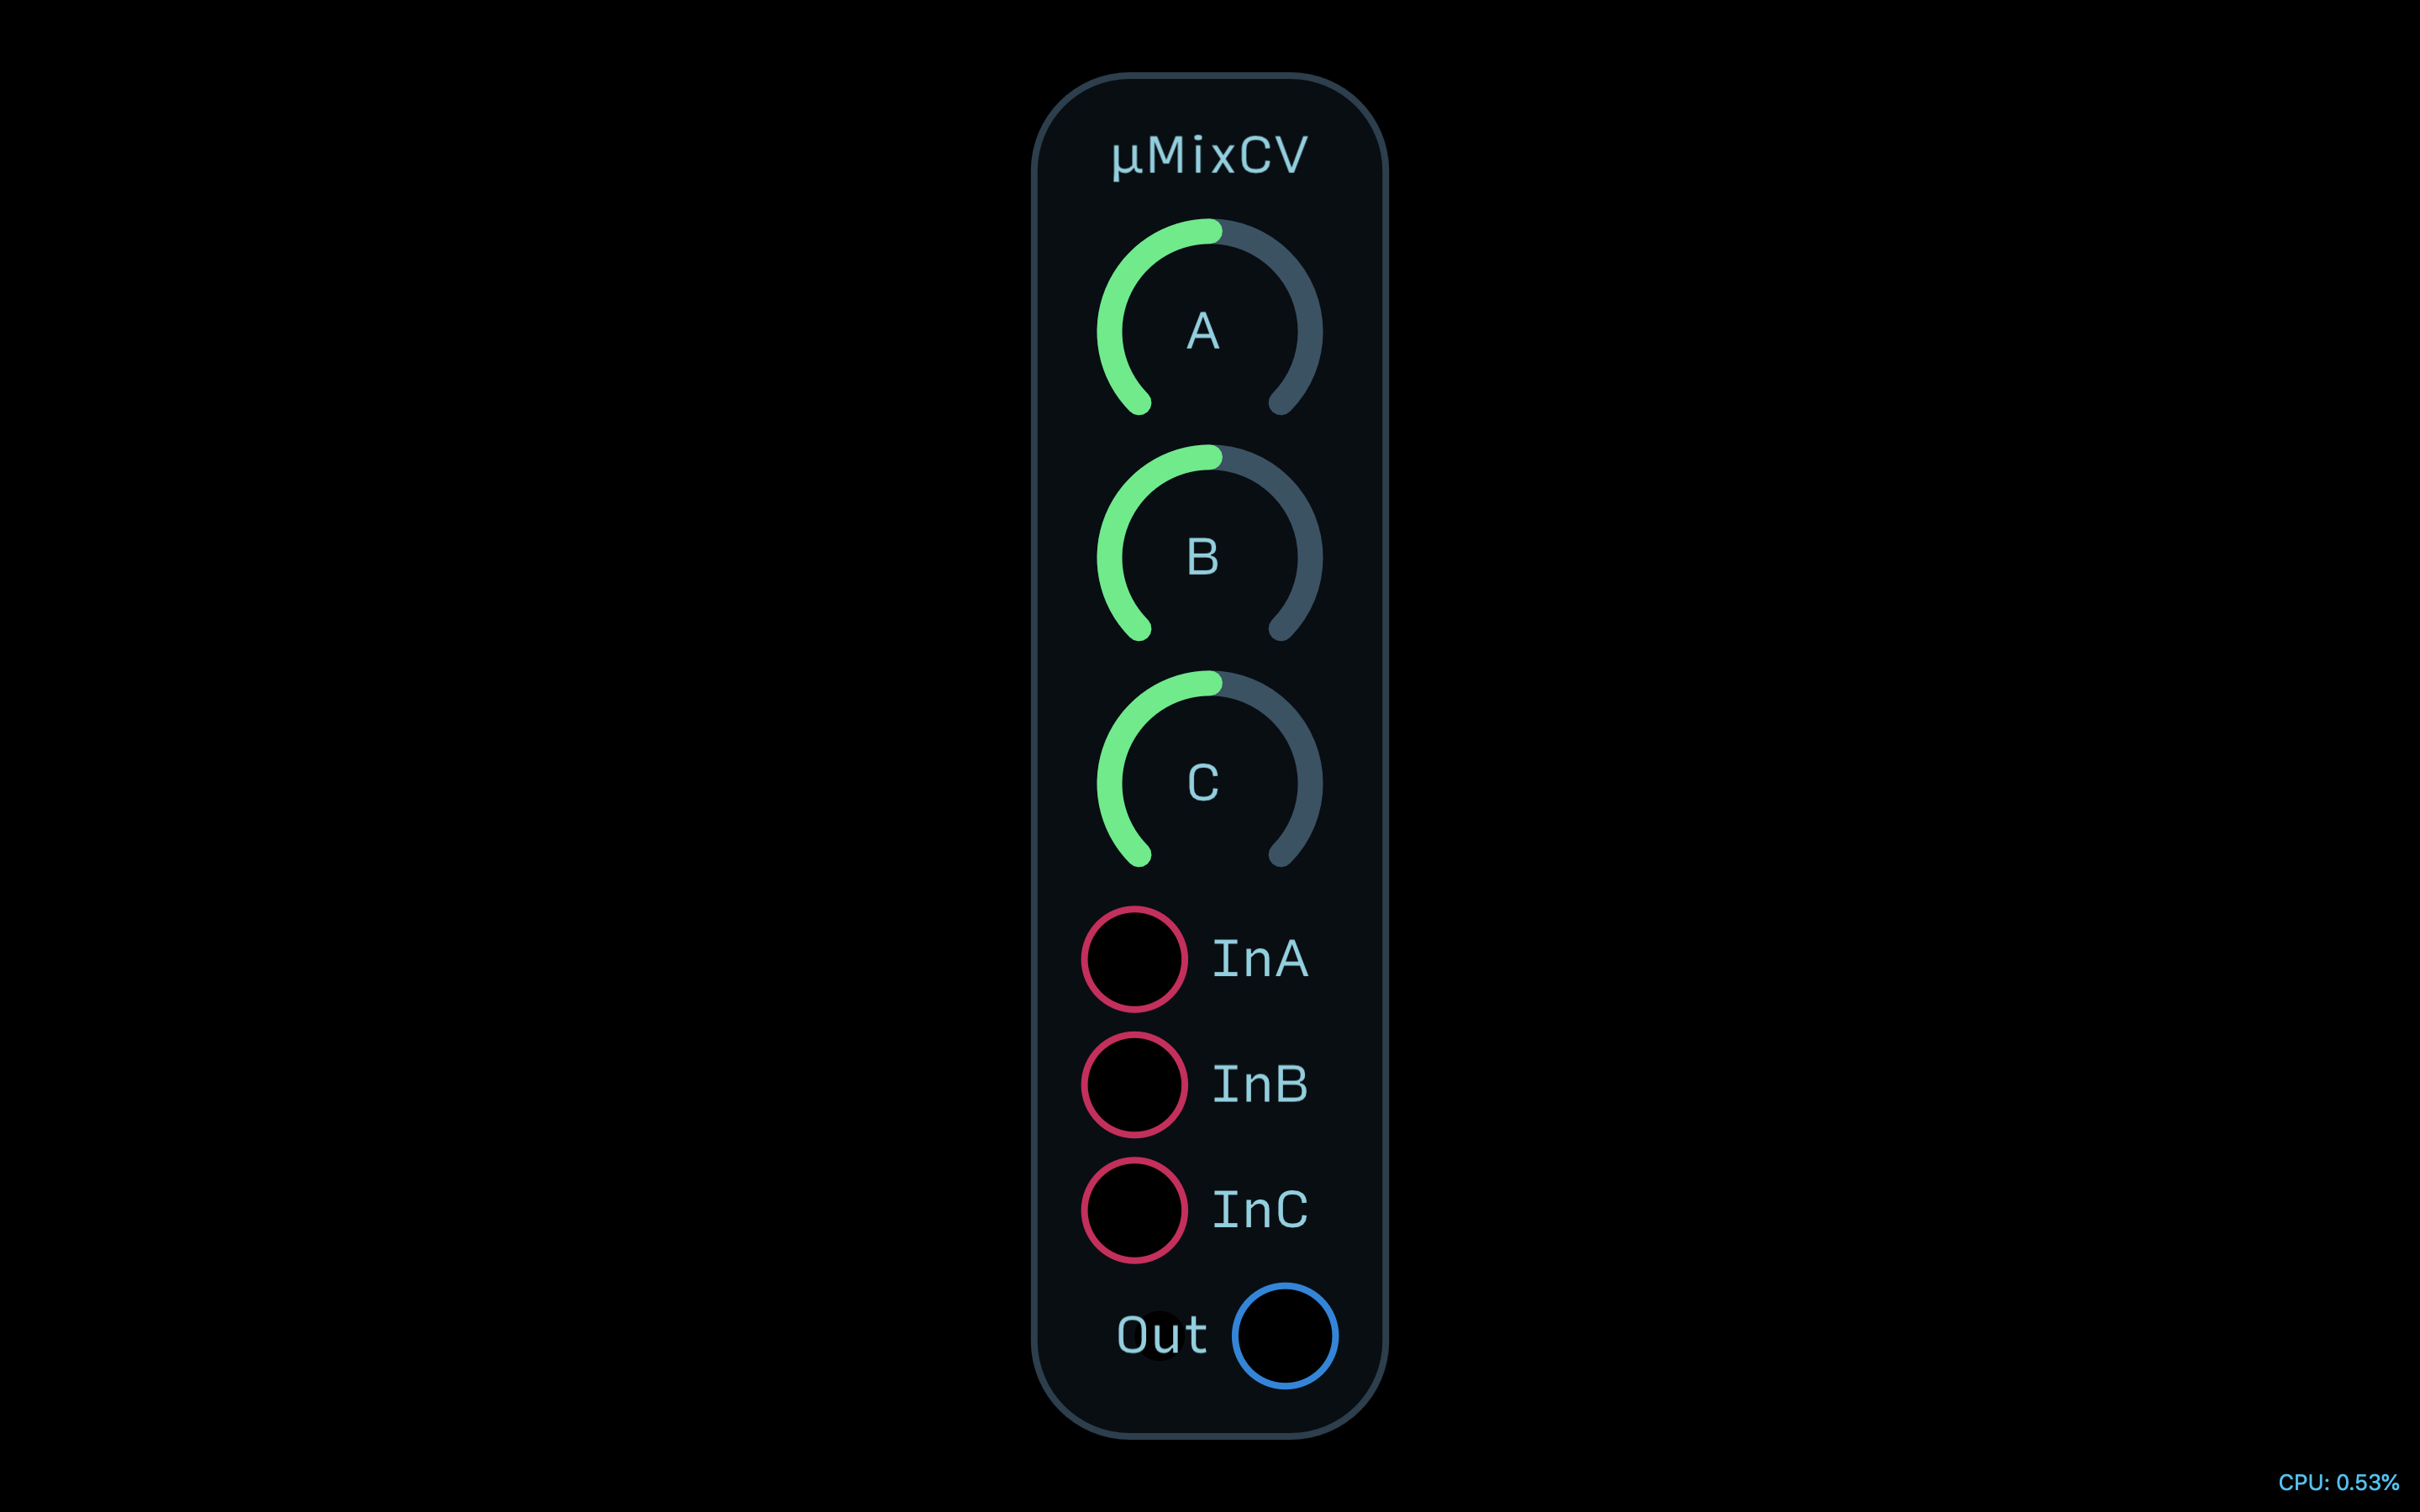
\includegraphics[width=\textwidth]{umix-cv.png}

\begin{table}[ht]
\small
\sffamily
\renewcommand\arraystretch{1.5}
\centering
\begin{tabular}{l*{1}{>{\raggedright\arraybackslash}p{0.7\linewidth}}}

\toprule
\textbf{Knob} \\
In A/B/C & \textit{Modulation input attenuators.} \\

\midrule
\textbf{Input} \\
In A/B/C & \textit{Modulation inputs.} \\

\midrule
\textbf{Output} \\
Out & \textit{Mixed modulation output. Note: Clips output to maximum 0 to 1 modulation range.} \\

\bottomrule
\end{tabular}
\end{table}% \\

\pagebreak


\chapter{Quantizer Modules}
\pagebreak

\section{Chromatic Quantizer}

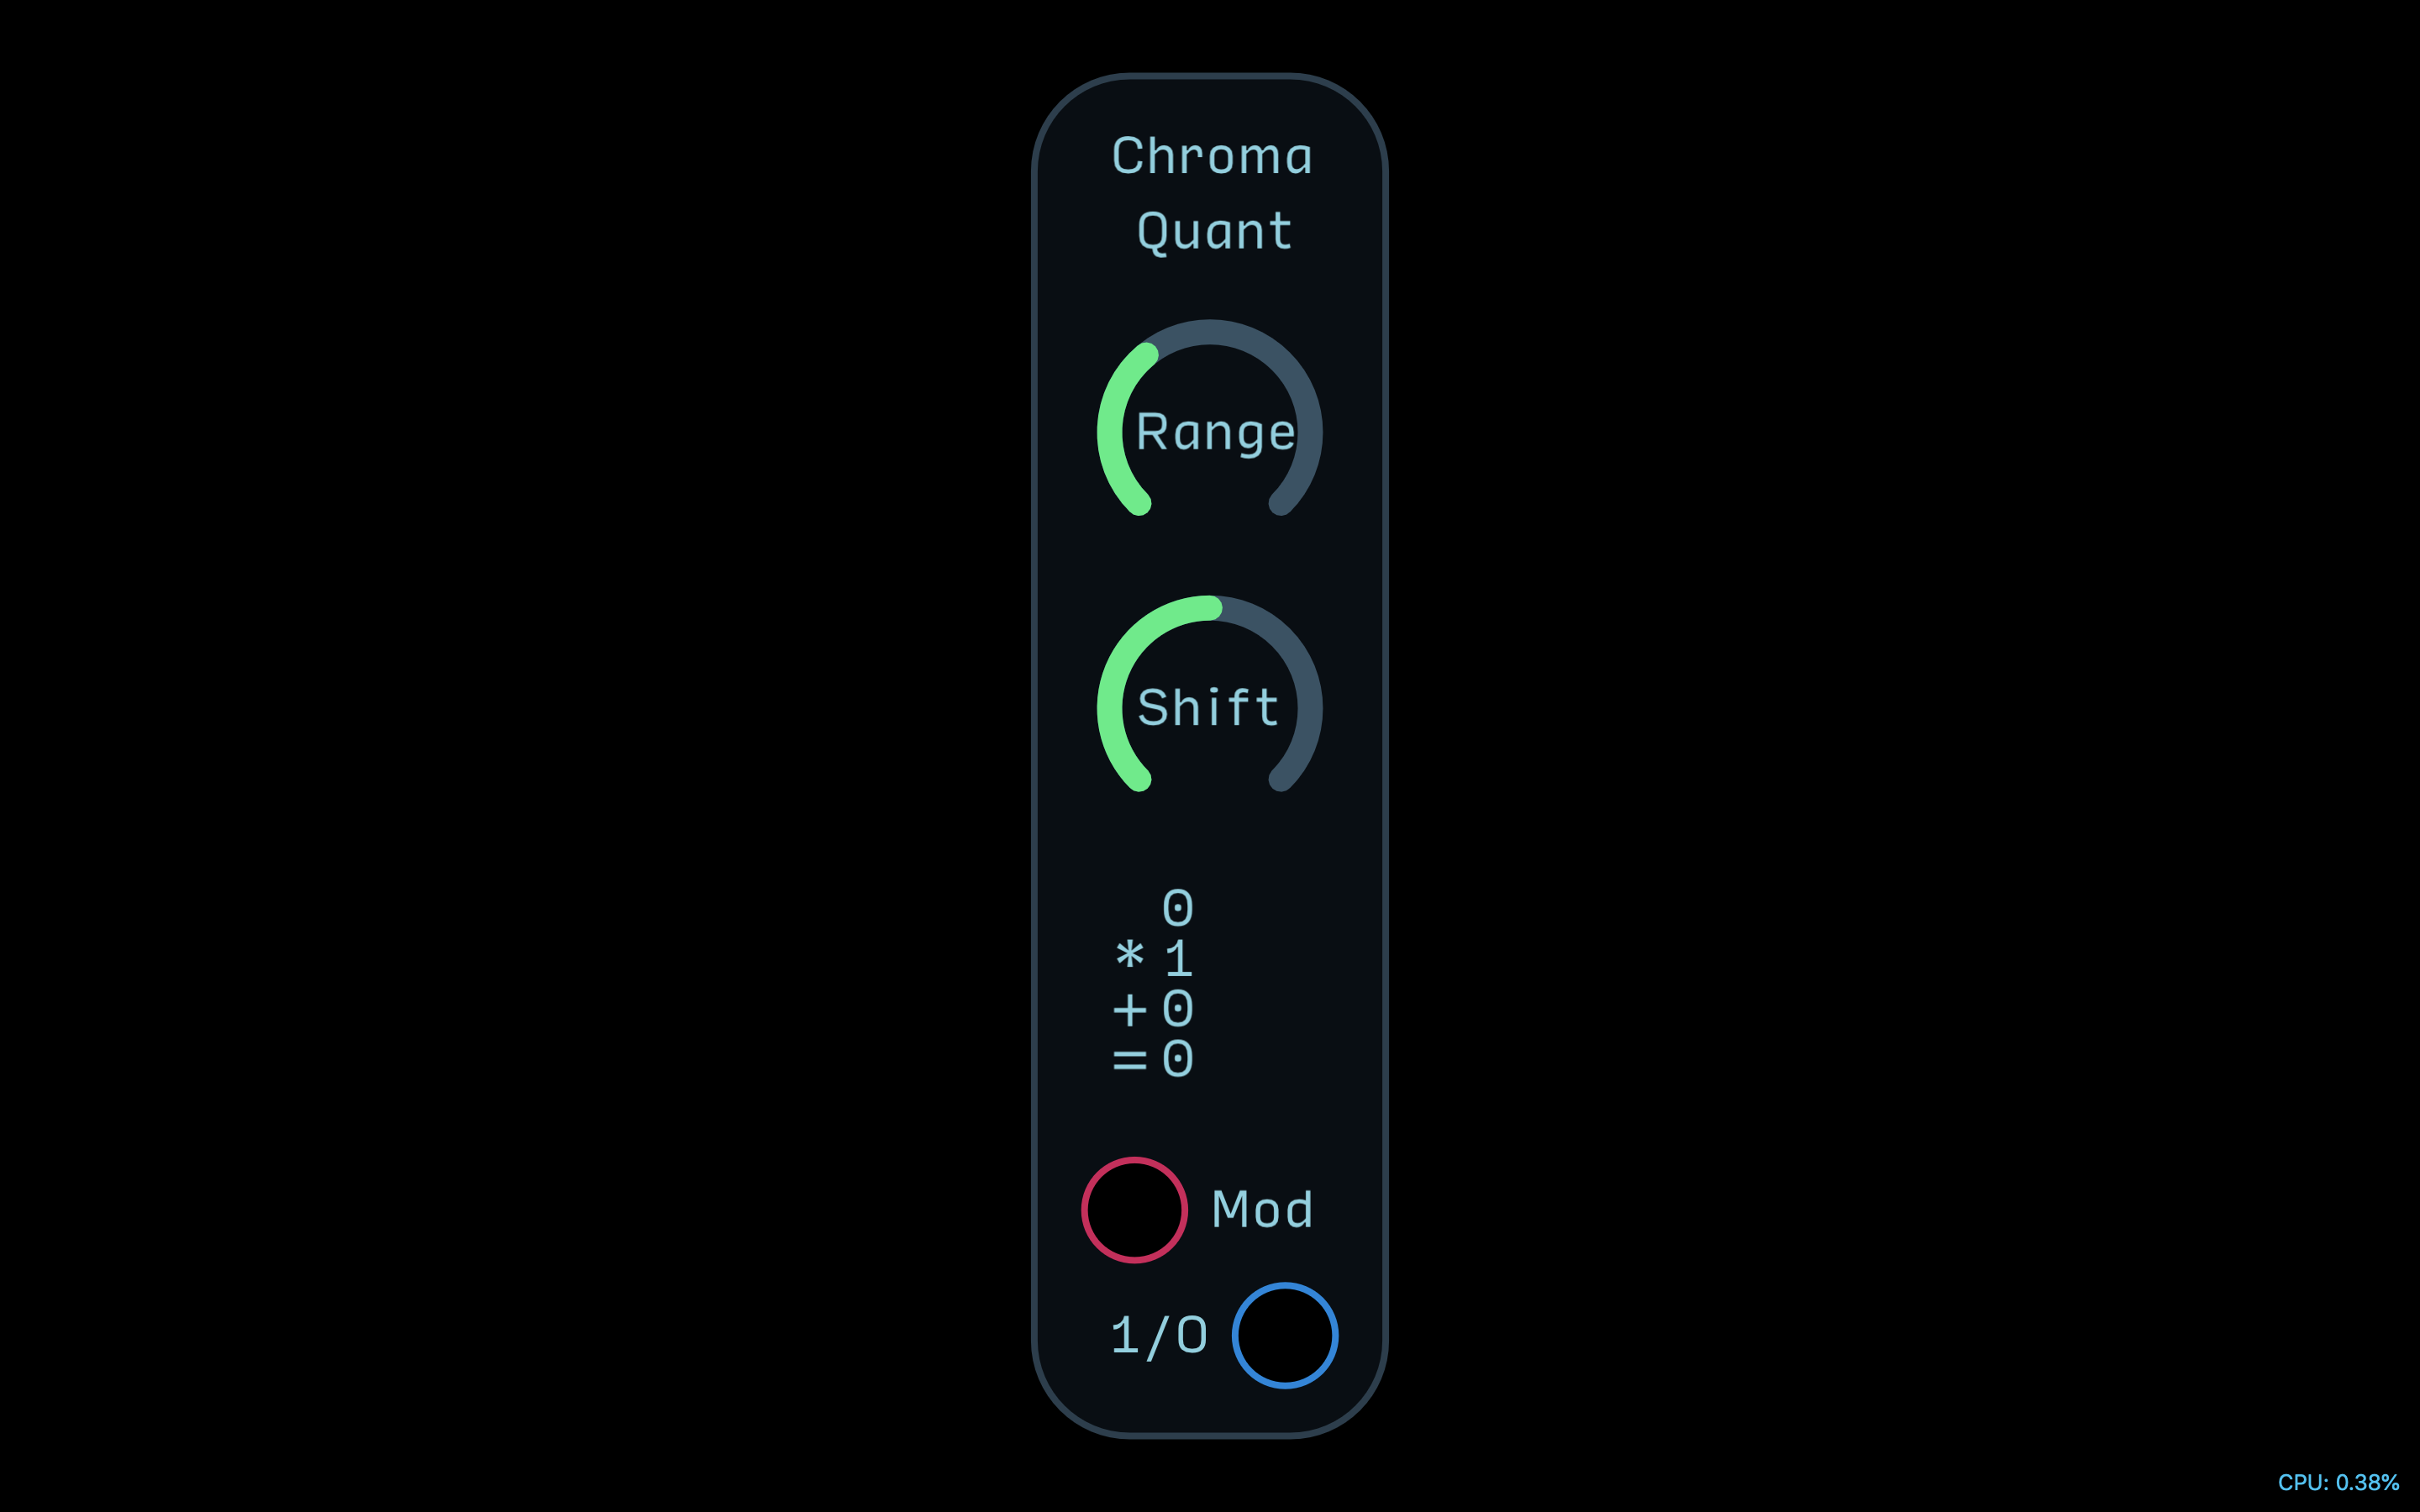
\includegraphics[width=\textwidth]{chromatic-quantizer.png}

\begin{table}[ht]
\small
\sffamily
\renewcommand\arraystretch{1.5}
\centering
\begin{tabular}{l*{1}{>{\raggedright\arraybackslash}p{0.7\linewidth}}}

\toprule
\textbf{Knob} \\
Range & \textit{Adjusts how many octaves the 1/Octave signal covers.} \\
Shift & \textit{Shifts the 1/Octave signal up and down.} \\

\midrule
\textbf{Input} \\
Mod & \textit{Modulation input.} \\

\midrule
\textbf{Output} \\
1/O & \textit{Quantized 1/Octave output.} \\

\bottomrule
\end{tabular}
\end{table}% \\

\pagebreak


\section{Church Modes Quantizer}

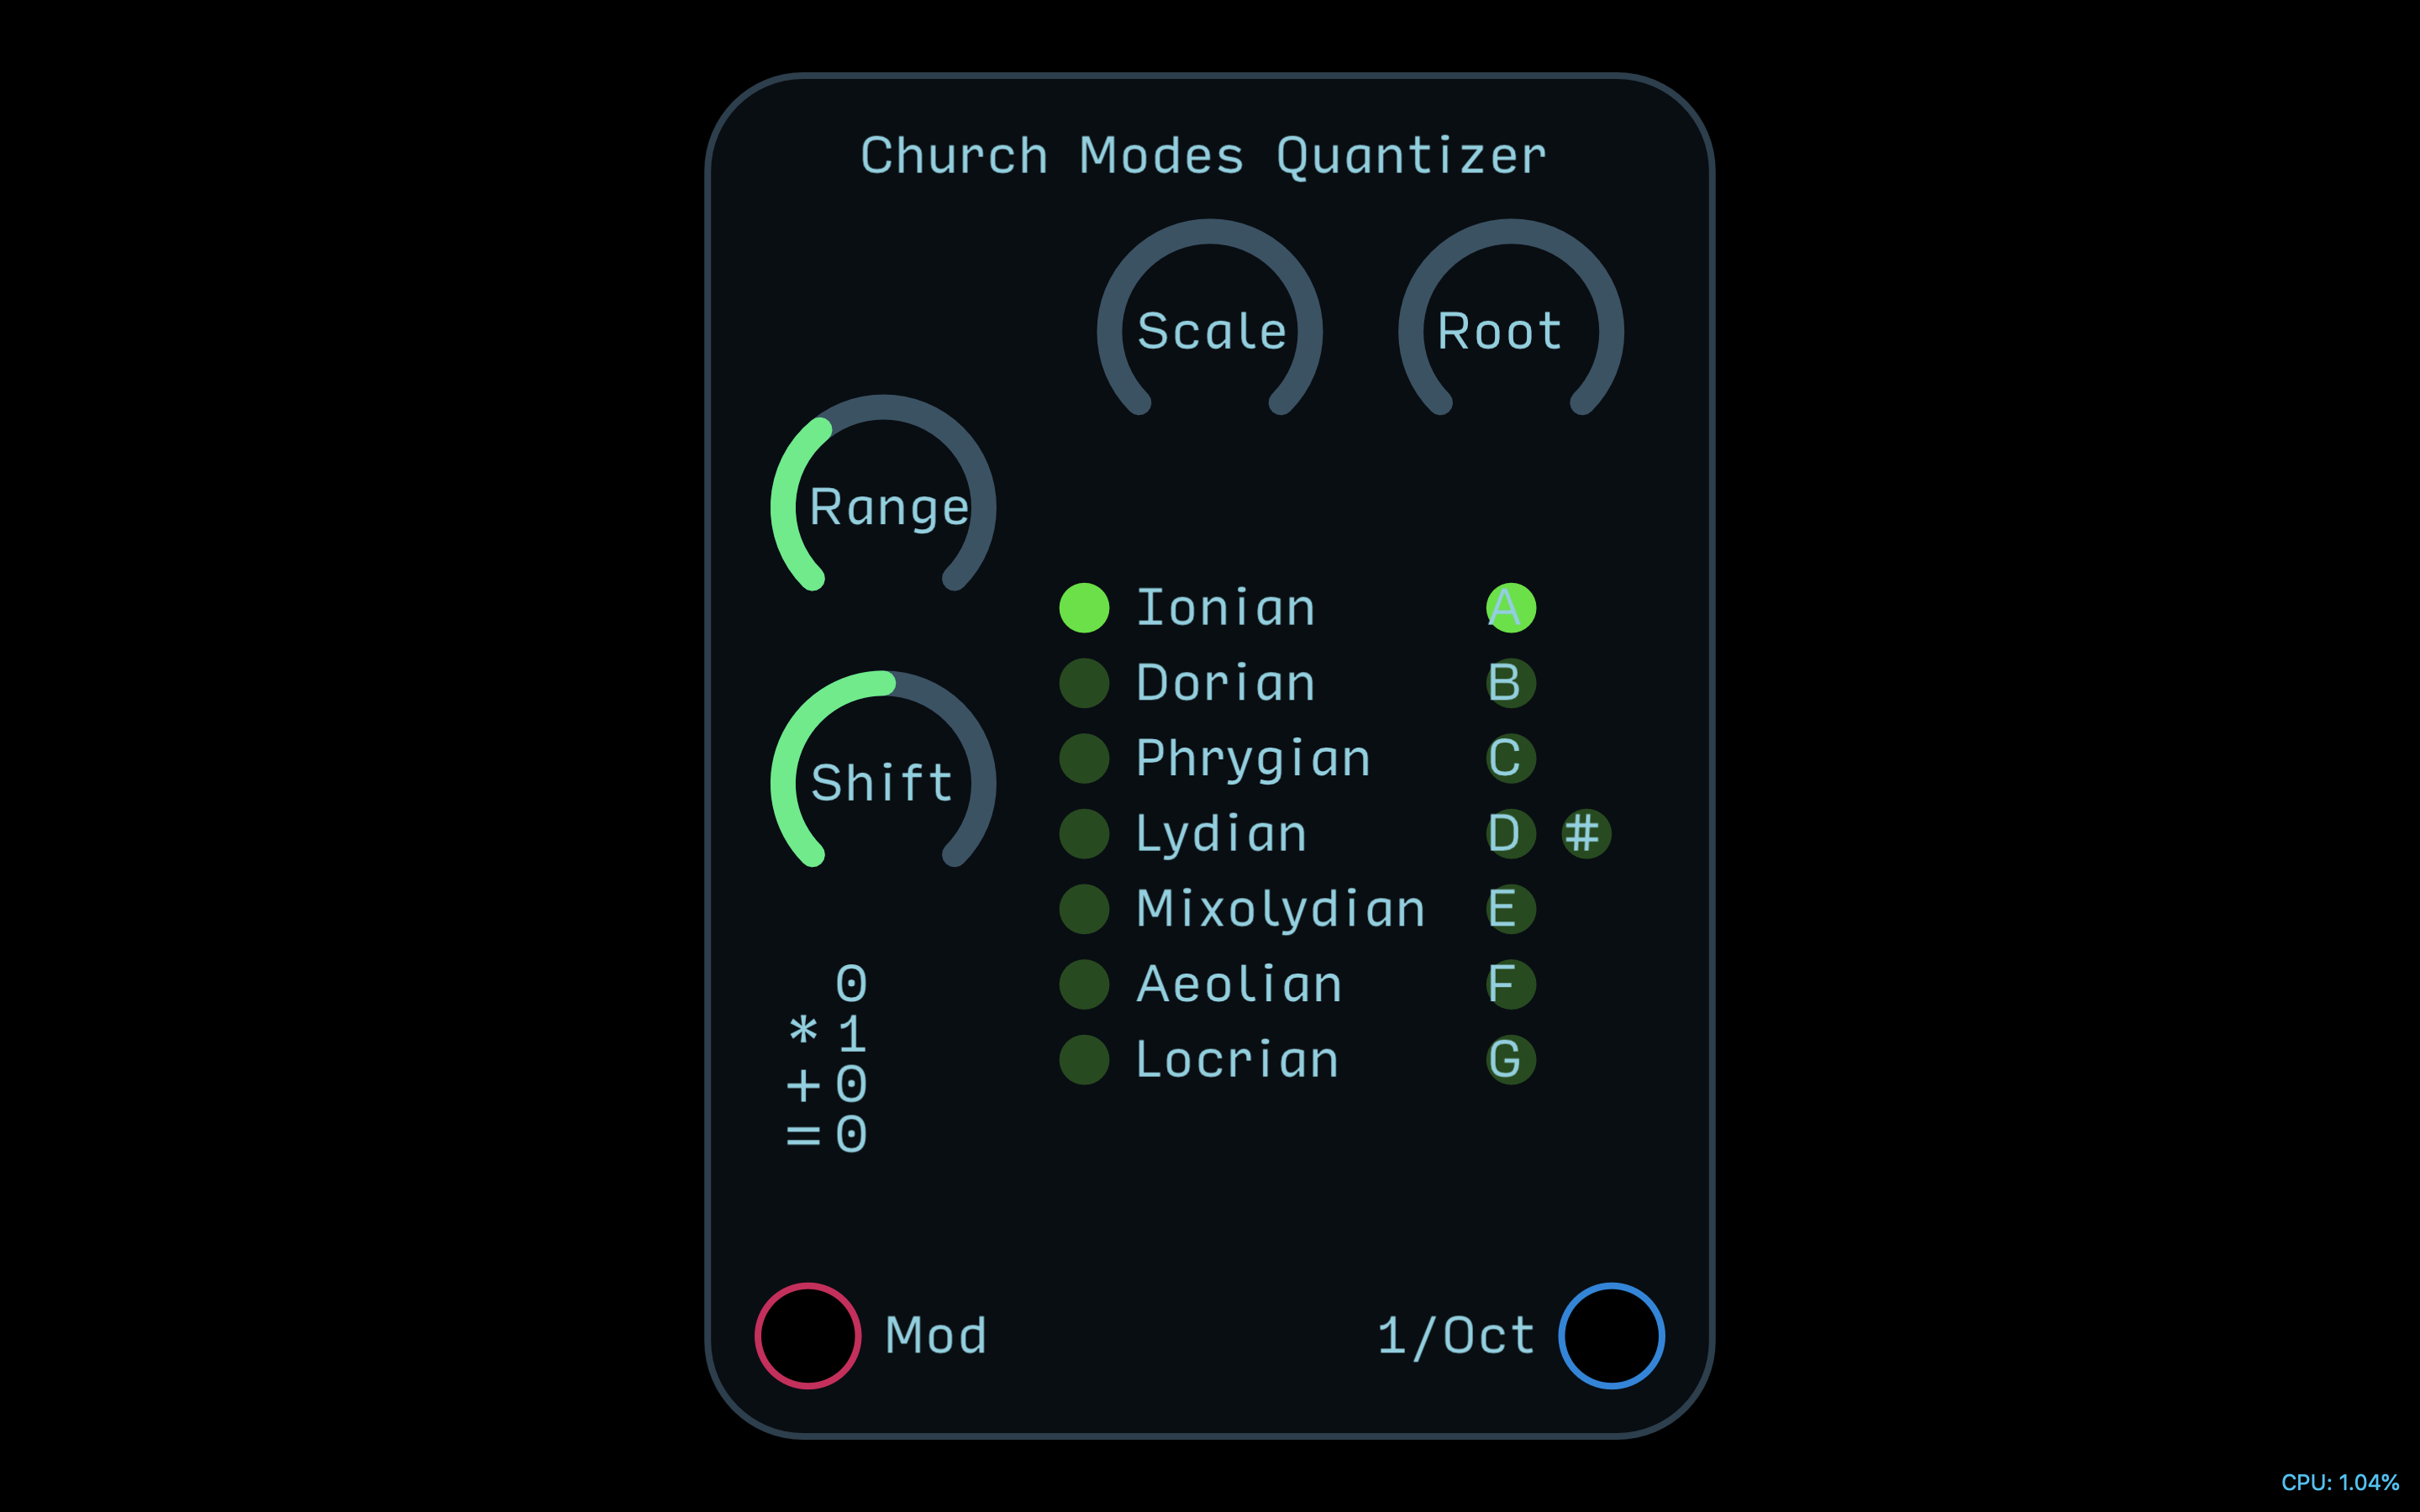
\includegraphics[width=\textwidth]{church-modes-quantizer.png}

\begin{table}[ht]
\small
\sffamily
\renewcommand\arraystretch{1.5}
\centering
\begin{tabular}{l*{1}{>{\raggedright\arraybackslash}p{0.7\linewidth}}}

\toprule
\textbf{Knob} \\
Scale & \textit{Adjusts the type of scale.} \\
Root & \textit{Shifts the root note of the quantizer. Note: If you need a scale in $B\flat$ use $A\sharp$, and so on.} \\
Range & \textit{Adjusts how many octaves the 1/Octave signal covers.} \\
Shift & \textit{Shifts the 1/Octave signal up and down.} \\

\midrule
\textbf{Input} \\
Mod & \textit{Modulation input.} \\

\midrule
\textbf{Output} \\
1/Oct & \textit{Quantized 1/Octave output.} \\

\bottomrule
\end{tabular}
\end{table}% \\

\pagebreak


\section{Gateable Quantizer}

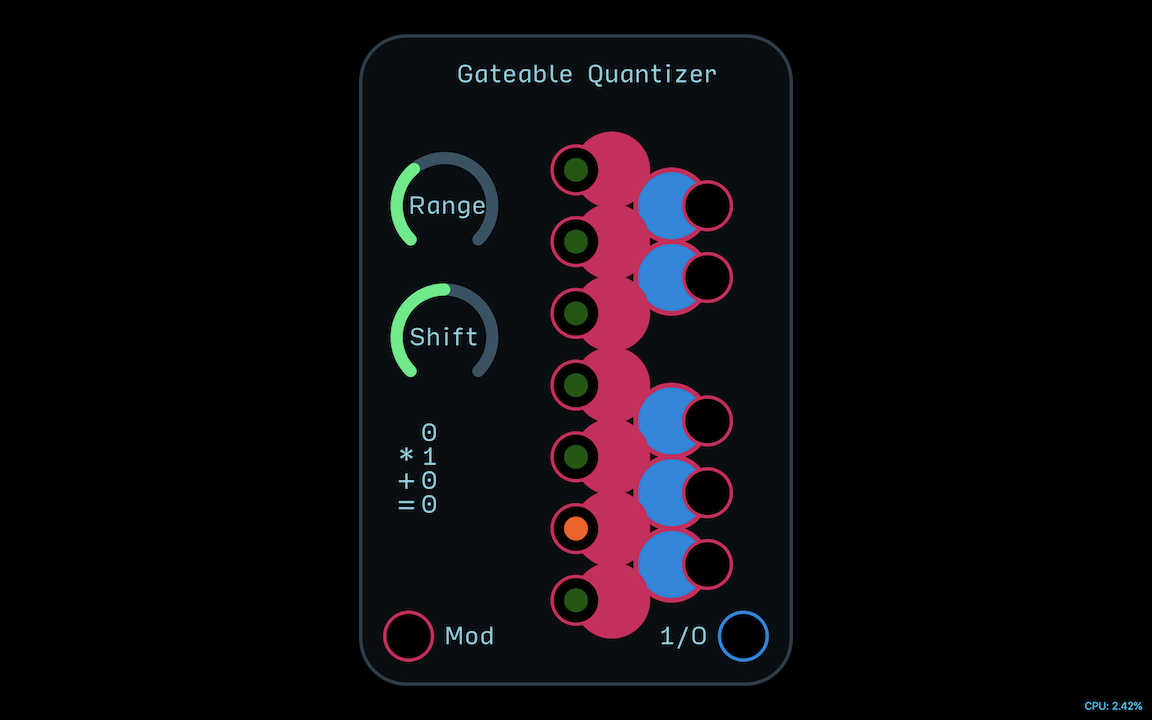
\includegraphics[width=\textwidth]{gateable-quantizer.png}

\begin{table}[ht]
\small
\sffamily
\renewcommand\arraystretch{1.5}
\centering
\begin{tabular}{l*{1}{>{\raggedright\arraybackslash}p{0.7\linewidth}}}

\toprule
\textbf{Knob} \\
Range & \textit{Adjusts how many octaves the 1/Octave signal covers.} \\
Shift & \textit{Shifts the 1/Octave signal up and down.} \\

\midrule
\textbf{Button} \\
Scale buttons & \textit{Switch buttons on to make notes active. Also includes a gateable input at each button that will remotely switch notes on and off so long as the button is turned off.} \\

\midrule
\textbf{Input} \\
Mod & \textit{Modulation input.} \\

\midrule
\textbf{Output} \\
1/O & \textit{Quantized 1/Octave output.} \\

\bottomrule
\end{tabular}
\end{table}% \\

\pagebreak


\section{Modulation Quantizer}

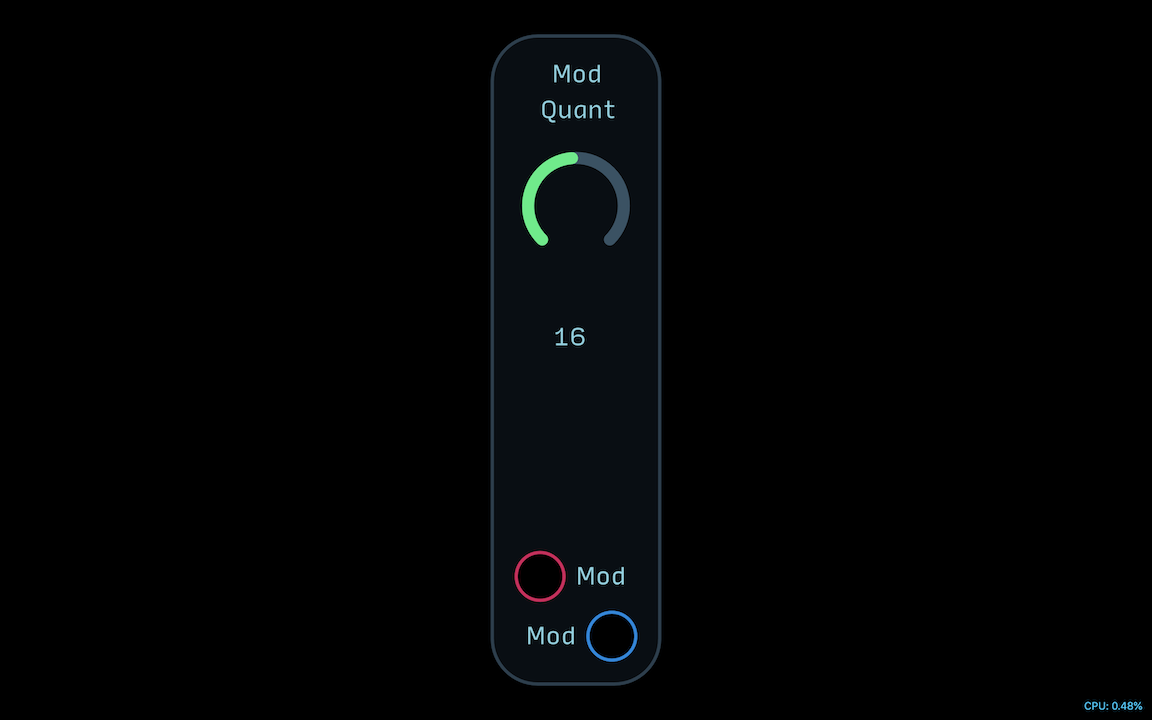
\includegraphics[width=\textwidth]{modulation-quantizer.png}

\begin{table}[ht]
\small
\sffamily
\renewcommand\arraystretch{1.5}
\centering
\begin{tabular}{l*{1}{>{\raggedright\arraybackslash}p{0.7\linewidth}}}

\toprule
\textbf{Knob} \\
Unlabeled knob & \textit{Sets the number of quantization levels from 2 to 64.} \\

\midrule
\textbf{Input} \\
Mod & \textit{Modulation input.} \\

\midrule
\textbf{Output} \\
Mod & \textit{Quantized modulation output.} \\

\bottomrule
\end{tabular}
\end{table}% \\

\pagebreak


\section{Neo-Reimannian Triad Transformer}

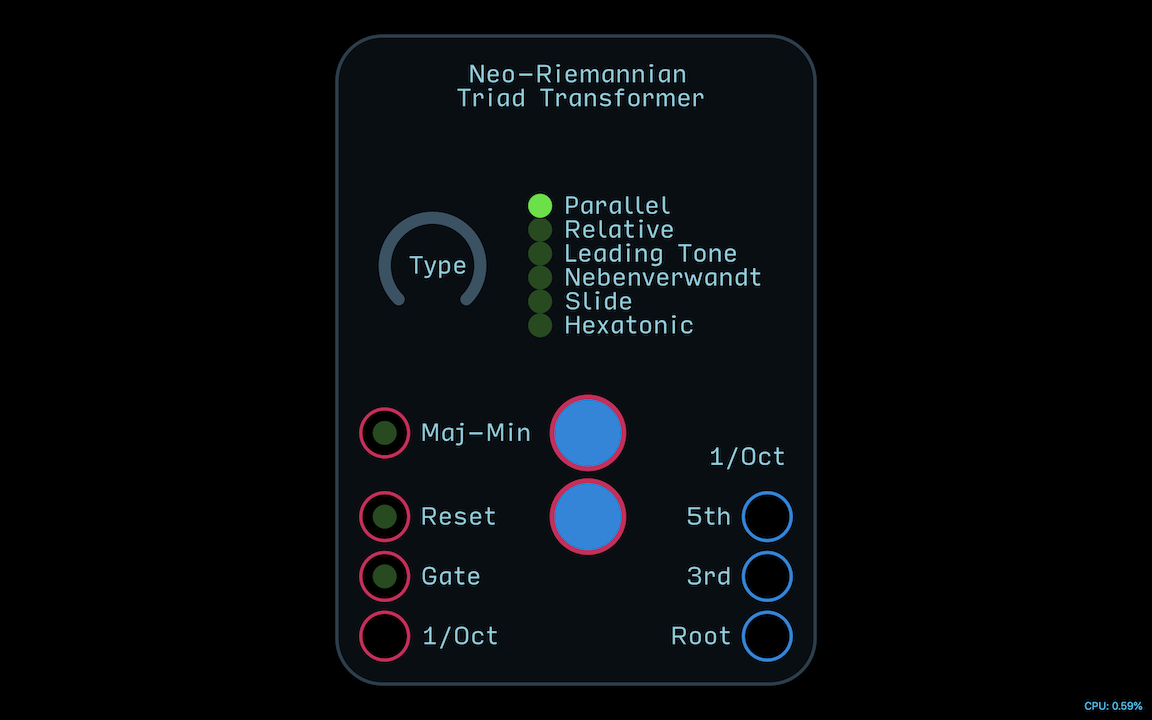
\includegraphics[width=\textwidth]{neo-reimannian-triad-transformer.png}

\begin{table}[ht]
\small
\sffamily
\renewcommand\arraystretch{1.5}
\centering
\begin{tabular}{l*{1}{>{\raggedright\arraybackslash}p{0.7\linewidth}}}

\toprule
\textbf{Knob} \\
Type & \textit{Sets the type of triad transformation indicated next to the knob.} \\

\midrule
\textbf{Input} \\
Maj-Min & \textit{Low gate input = Major; high gate input = minor. The button next to the input will switch between major (off) and minor (on) as well.} \\
Reset & \textit{Resets the transformation algorithm. The button next to the input can also be pushed to manually reset.} \\
Gate & \textit{Triggers a new triad transformation.} \\
1/Oct & \textit{1/Octave input.} \\

\midrule
\textbf{Output} \\
1/Oct Root/3rd/5th & \textit{Quantized 1/Octave root, 3rd and 5th notes.} \\

\bottomrule
\end{tabular}
\end{table}% \\

\pagebreak


\section{Quick Quantizer}

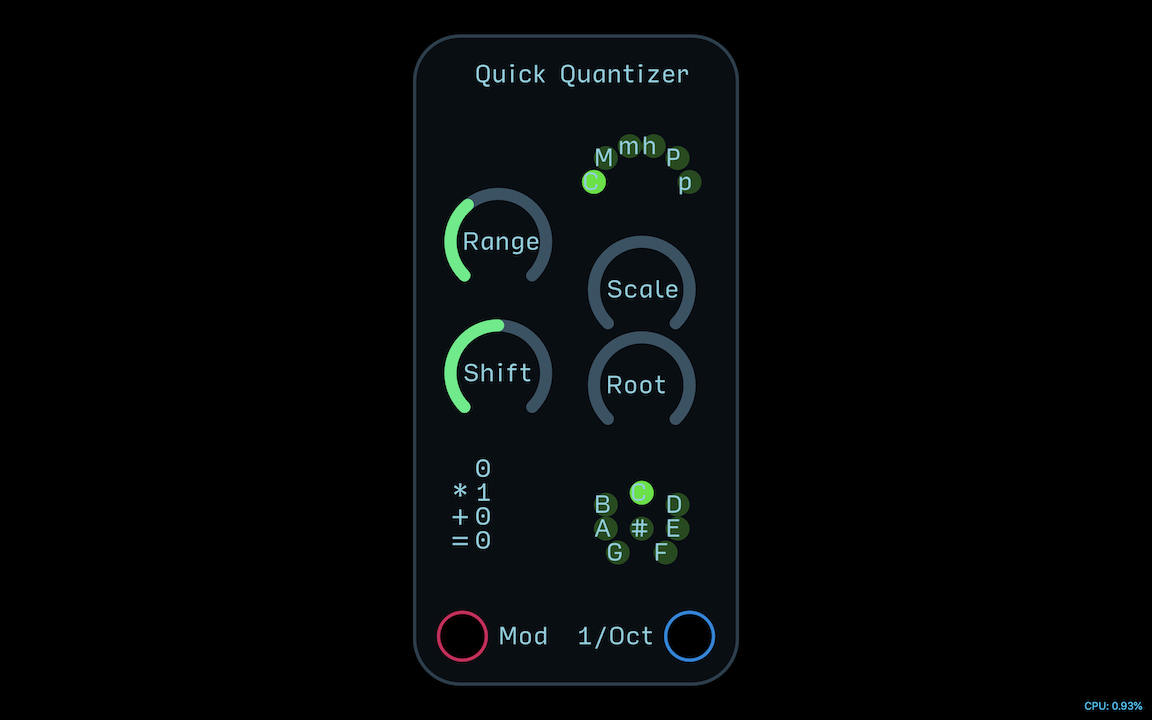
\includegraphics[width=\textwidth]{quick-quantizer.png}

\begin{table}[ht]
\small
\sffamily
\renewcommand\arraystretch{1.5}
\centering
\begin{tabular}{l*{1}{>{\raggedright\arraybackslash}p{0.7\linewidth}}}

\toprule
\textbf{Knob} \\
Range & \textit{Adjusts how many octaves the 1/Octave signal covers.} \\
Shift & \textit{Shifts the 1/Octave signal up and down.} \\
Scale & \textit{Adjusts the type of scale: (C)hromatic, (M)ajor, (m)inor, (h)armonic minor, (P)entatonic major, (p)entatonic minor.} \\
Root & \textit{Shifts the root note of the quantizer. Note: If you need a scale in $B\flat$ use $A\sharp$, and so on.} \\

\midrule
\textbf{Input} \\
Mod & \textit{Modulation input.} \\

\midrule
\textbf{Output} \\
1/Oct & \textit{Quantized 1/Octave output.} \\

\bottomrule
\end{tabular}
\end{table}% \\

\pagebreak


\chapter{Sequencer Modules}
\pagebreak


\section{16 Step Gate Sequencer}

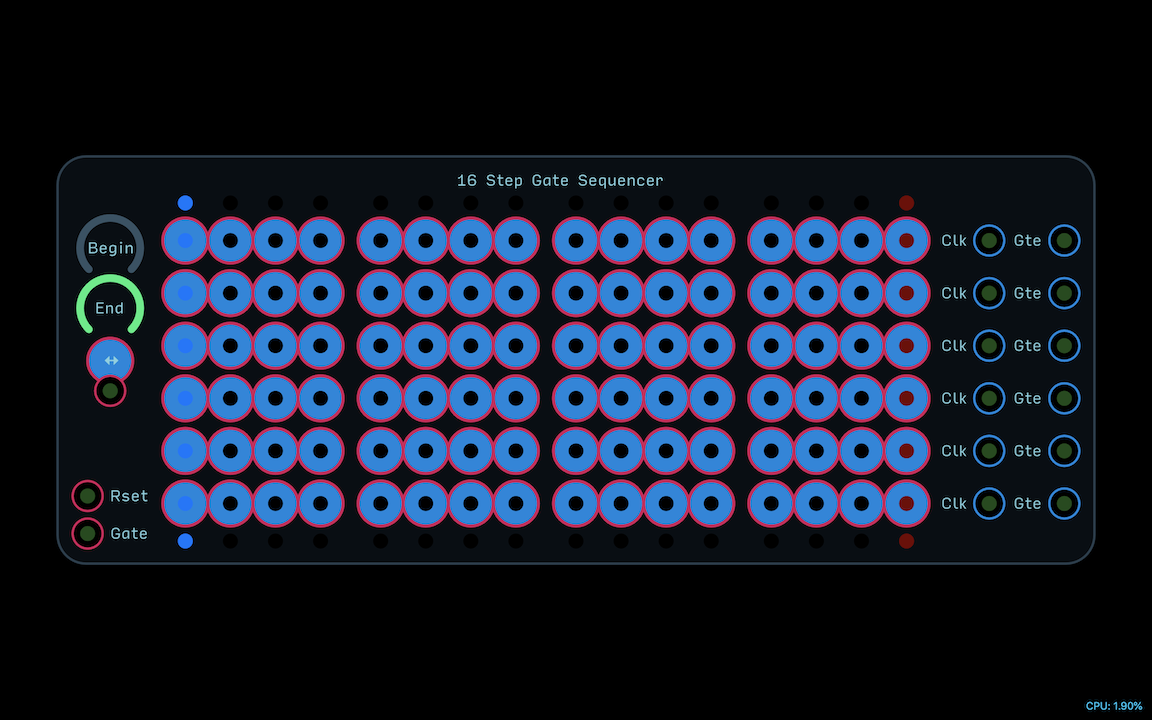
\includegraphics[width=\textwidth]{16-step-gate-sequencer.png}

\begin{table}[ht]
\small
\sffamily
\renewcommand\arraystretch{1.5}
\centering
\begin{tabular}{l*{1}{>{\raggedright\arraybackslash}p{0.7\linewidth}}}

\toprule
\textbf{Knob} \\
Begin/End & \textit{Sets the beginning and end of the sequence. To reverse sequence, set Begin to higher than End.} \\

\midrule
\textbf{Button} \\
Field of 6x16 buttons & \textit{6 lanes of 16 step sequences. Press button to turn step on.} \\
$\leftrightarrow$ & \textit{Turns on ping-pong mode. Can be gated externally as long as button is turned off.} \\

\midrule
\textbf{Input} \\
Rset & \textit{Restart sequencer from Begin step.} \\
Gate & \textit{Steps sequencer forward.} \\

\midrule
\textbf{Output} \\
Clk & \textit{Outputs the incoming clock if step is engaged.} \\
Gate & \textit{Outputs a gate based on current step, e.g., if 4 steps in a row are pressed, the gate will stay high the duration of those 4 steps.} \\

\bottomrule
\end{tabular}
\end{table}% \\

\pagebreak


\section{8 Step Sequencer}

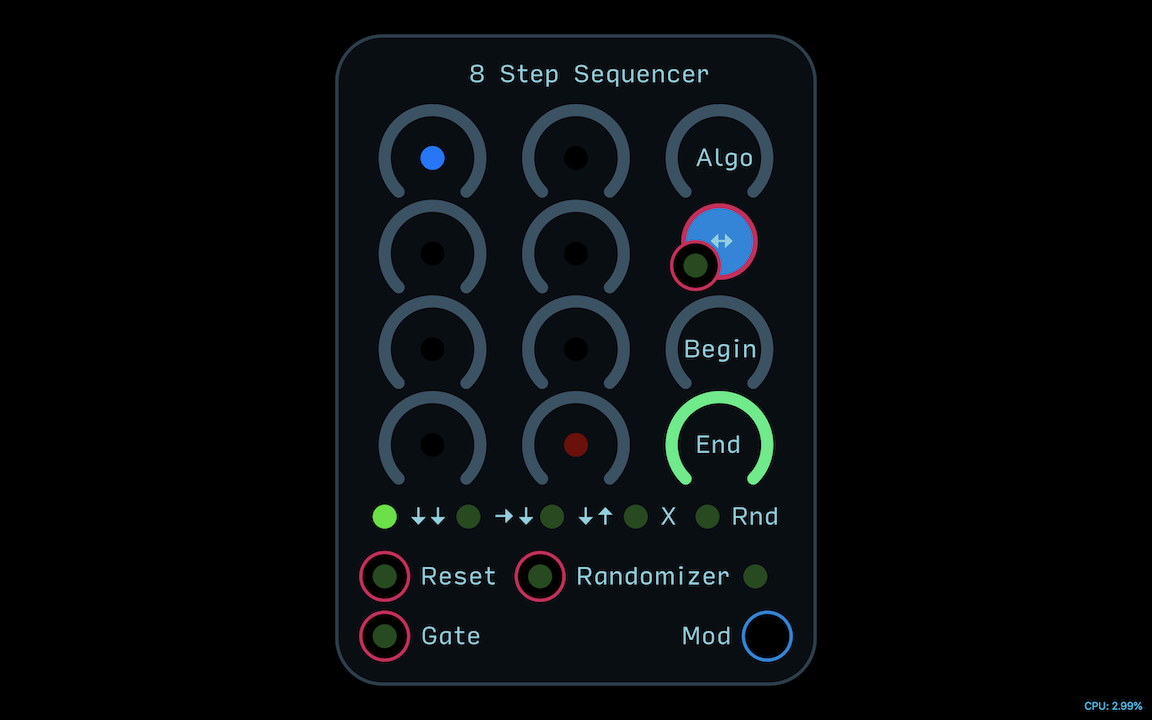
\includegraphics[width=\textwidth]{8-step-sequencer.png}

\begin{table}[ht]
\small
\sffamily
\renewcommand\arraystretch{1.5}
\centering
\begin{tabular}{l*{1}{>{\raggedright\arraybackslash}p{0.7\linewidth}}}

\toprule
\textbf{Knob} \\
x8 Unmarked Knobs & \textit{Sequencer step values.} \\
Algo & \textit{Adjusts the sequencer pattern algorithm, indicated by the lights at the bottom of the sequencer. $\downarrow \downarrow$ = Top to bottom, left to right. $\rightarrow \downarrow$ = Left to right, top to bottom. $\downarrow \uparrow$ = Top to bottom, bottom to top. $X$ = crosswise pattern. $Rnd$ = Steps chosen at random. $Randomizer$ = Random chance mode. Knobs set \% chance that new random value will be selected when Randomizer input is gated.} \\
Begin/End & \textit{Sets the beginning and end of the sequence. To reverse sequence, set Begin to higher than End.} \\

\midrule
\textbf{Button} \\
$\leftrightarrow$ & \textit{Turns on ping-pong mode. Can be gated externally as long as button is turned off.} \\

\midrule
\textbf{Input} \\
Reset & \textit{Restart sequencer from Begin step.} \\
Randomizer & \textit{Randomizes step values when Randomizer algo is selected.} \\
Gate & \textit{Steps sequencer forward.} \\

\midrule
\textbf{Output} \\
Mod & \textit{Modulation output.} \\

\bottomrule
\end{tabular}
\end{table}% \\

\pagebreak


\section{Binary Gate Sequencer}

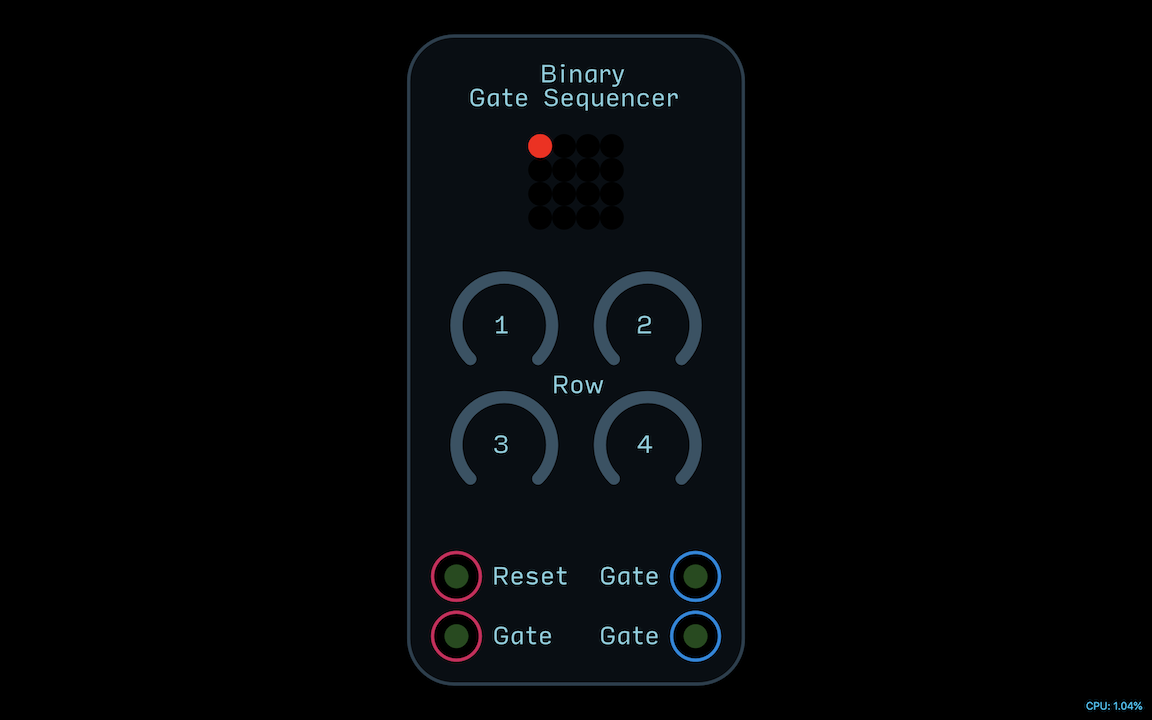
\includegraphics[width=\textwidth]{binary-gate-sequencer.png}

\begin{table}[ht]
\small
\sffamily
\renewcommand\arraystretch{1.5}
\centering
\begin{tabular}{l*{1}{>{\raggedright\arraybackslash}p{0.7\linewidth}}}

\toprule
\textbf{Knob} \\
1/2/3/4 & \textit{Each knob changes the on/off combination of steps for each row as indicated by the lights above.} \\

\midrule
\textbf{Input} \\
Reset & \textit{Restart sequencer from beginning.} \\
Gate & \textit{Steps sequencer forward.} \\

\midrule
\textbf{Output} \\
Clock & \textit{Outputs the incoming clock if step is engaged.} \\
Gate & \textit{Outputs a gate based on current step, e.g., if 4 steps in a row are engaged, the gate will stay high the duration of those 4 steps.} \\

\bottomrule
\end{tabular}
\end{table}% \\

\pagebreak


\section{Euclidean Gate Sequencer}

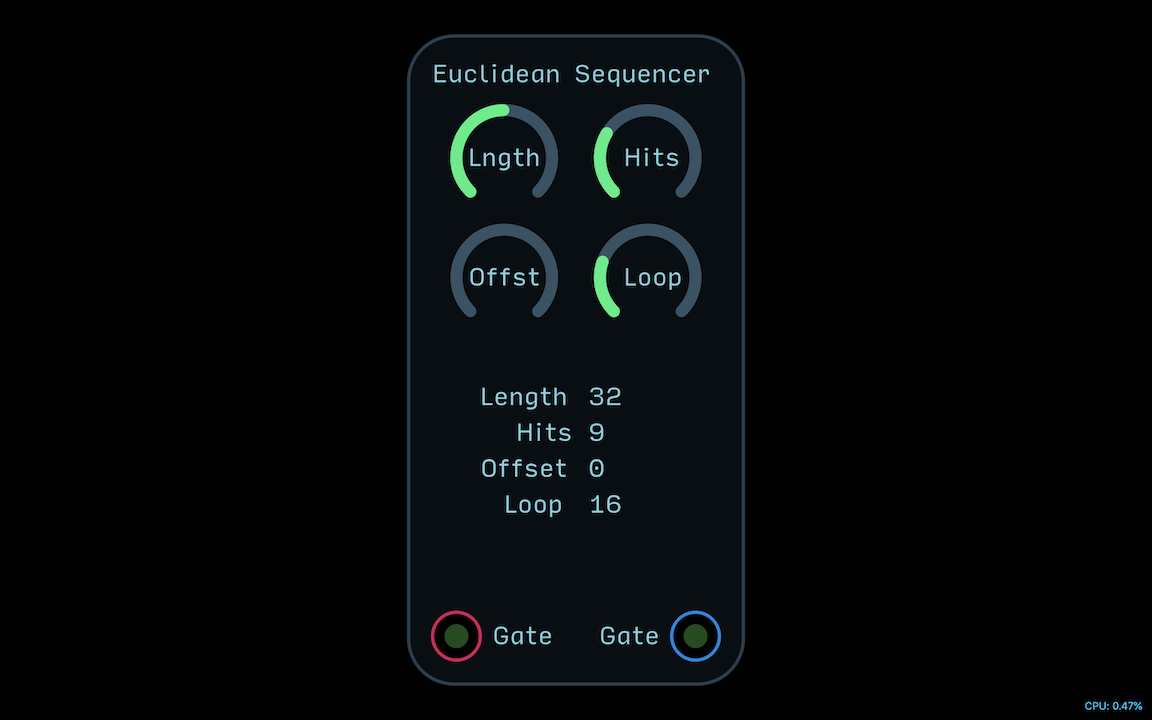
\includegraphics[width=\textwidth]{euclidean-gate-sequencer.png}

\begin{table}[ht]
\small
\sffamily
\renewcommand\arraystretch{1.5}
\centering
\begin{tabular}{l*{1}{>{\raggedright\arraybackslash}p{0.7\linewidth}}}

\toprule
\textbf{Knob} \\
Lngth & \textit{Length of Euclidean pattern.} \\
Hits & \textit{Density of hits within pattern.} \\
Offst & \textit{Offsets the pattern's starting point.} \\
Loop & \textit{Allows you to clip out a sub portion of the total length in more musically-useful subdivisions and loop it.} \\

\midrule
\textbf{Input} \\
Gate & \textit{Steps sequencer forward.} \\

\midrule
\textbf{Output} \\
Gate & \textit{Outputs a gate based on current step, e.g., if 4 steps in a row are engaged, the gate will stay high the duration of those 4 steps.} \\

\bottomrule
\end{tabular}
\end{table}% \\

\pagebreak


\section{Matrix Gate Sequencer}

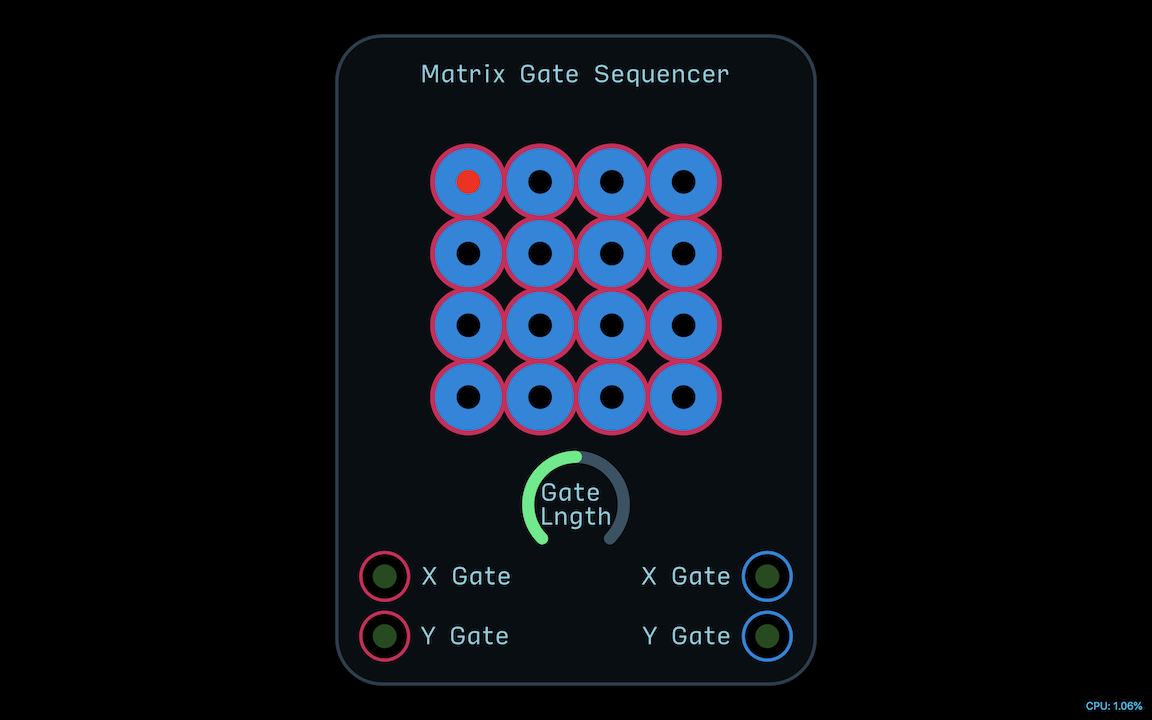
\includegraphics[width=\textwidth]{matrix-gate-sequencer.png}

\begin{table}[ht]
\small
\sffamily
\renewcommand\arraystretch{1.5}
\centering
\begin{tabular}{l*{1}{>{\raggedright\arraybackslash}p{0.7\linewidth}}}

\toprule
\textbf{Knob} \\
Gate Lngth & \textit{Length of output gates.} \\

\midrule
\textbf{Button} \\
4x4 Button Field & \textit{Turn button on to make step active.} \\

\midrule
\textbf{Input} \\
X/Y Gate & \textit{Steps sequencer forward on X or Y plane.} \\

\midrule
\textbf{Output} \\
X/Y Gate & \textit{Outputs a gate if current step is active.} \\

\bottomrule
\end{tabular}
\end{table}% \\

\pagebreak


\section{Shape Gate Sequencer}

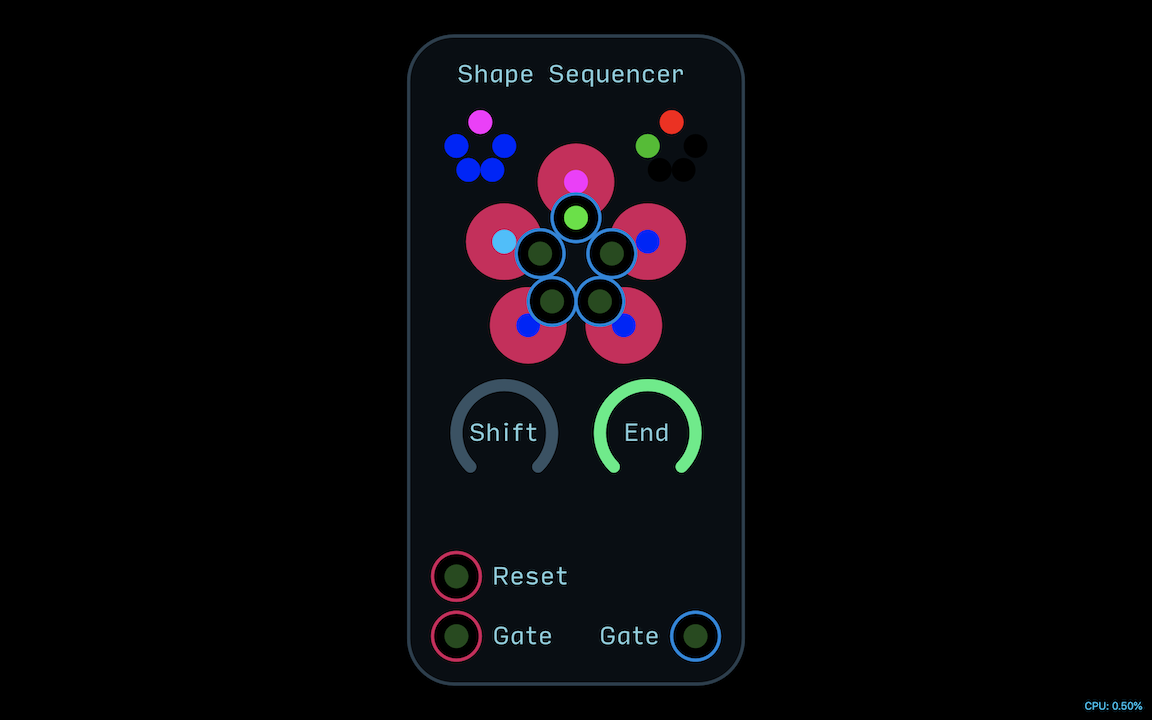
\includegraphics[width=\textwidth]{shape-gate-sequencer.png}

\begin{table}[ht]
\small
\sffamily
\renewcommand\arraystretch{1.5}
\centering
\begin{tabular}{l*{1}{>{\raggedright\arraybackslash}p{0.7\linewidth}}}

\toprule
\textbf{Knob} \\
Shift & \textit{Shifts the pattern set by the buttons clockwise.} \\
End & \textit{Sets the number of steps in the pattern.} \\

\midrule
\textbf{Button} \\
5 button circle & \textit{Push button to make step active. Each step has a gate output associated that will go high when the step is selected and active.} \\

\midrule
\textbf{Input} \\
Reset & \textit{Restart sequencer from beginning.} \\
Gate & \textit{Steps sequencer forward.} \\

\midrule
\textbf{Output} \\
Gate & \textit{Outputs a gate if current step is active.} \\

\bottomrule
\end{tabular}
\end{table}% \\

\pagebreak


\chapter{Utility Modules}
\pagebreak

\section{Attenuate-Offset}

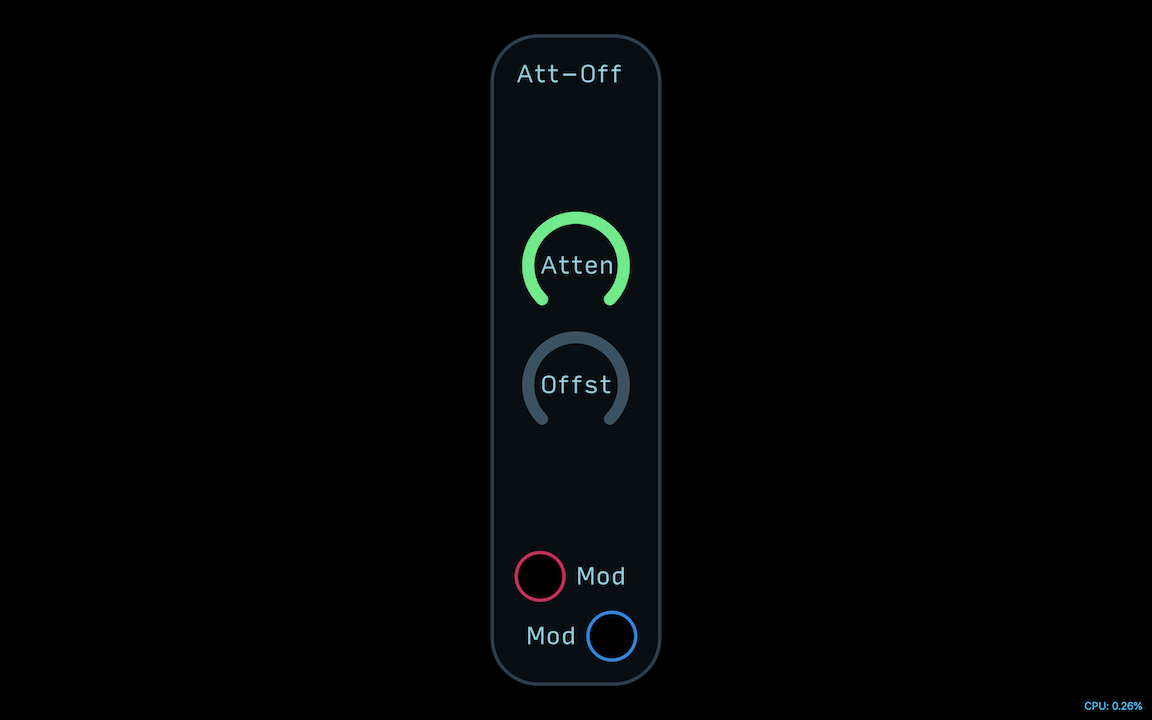
\includegraphics[width=\textwidth]{attenuate-offset.png}

\begin{table}[ht]
\small
\sffamily
\renewcommand\arraystretch{1.5}
\centering
\begin{tabular}{l*{1}{>{\raggedright\arraybackslash}p{0.7\linewidth}}}

\toprule
\textbf{Knob} \\
Atten & \textit{Attenuates incoming modulation signal.} \\
Offst & \textit{Shifts modulation signal up or down. Note: Modulation output will clip if output exceeds the 0 to 1 modulation range.} \\

\midrule
\textbf{Input} \\
Mod & \textit{Modulation input.} \\

\midrule
\textbf{Output} \\
Mod & \textit{Modulation output.} \\

\bottomrule
\end{tabular}
\end{table}% \\

\pagebreak

\section{Audio Attenuverter-Offset}

\includegraphics[width=\textwidth]{audio-attenuverter-offset.png}

\begin{table}[ht]
\small
\sffamily
\renewcommand\arraystretch{1.5}
\centering
\begin{tabular}{l*{1}{>{\raggedright\arraybackslash}p{0.7\linewidth}}}

\toprule
\textbf{Knob} \\
Attvt & \textit{Attenuverts incoming audio signal.} \\
Offst & \textit{Shifts audio signal up or down. Note: Modulation output will clip if output exceeds the 0 to 1 modulation range.} \\

\midrule
\textbf{Input} \\
In & \textit{Audio input.} \\

\midrule
\textbf{Output} \\
Out & \textit{Audio output.} \\

\bottomrule
\end{tabular}
\end{table}% \\

\pagebreak


\section{Attenuverter}

\includegraphics[width=\textwidth]{attenuverter.png}

\begin{table}[ht]
\small
\sffamily
\renewcommand\arraystretch{1.5}
\centering
\begin{tabular}{l*{1}{>{\raggedright\arraybackslash}p{0.7\linewidth}}}

\toprule
\textbf{Knob} \\
-/+ & \textit{Attenuverts incoming modulation signal while keeping it within the 0 to 1 modulation range.} \\

\midrule
\textbf{Input} \\
Mod & \textit{Modulation input.} \\

\midrule
\textbf{Output} \\
Mod & \textit{Modulation output.} \\

\bottomrule
\end{tabular}
\end{table}% \\

\pagebreak


\section{Automation Lane}

\includegraphics[width=\textwidth]{automation-lane.png}

\begin{table}[ht]
\small
\sffamily
\renewcommand\arraystretch{1.5}
\centering
\begin{tabular}{l*{1}{>{\raggedright\arraybackslash}p{0.7\linewidth}}}

\toprule
\textbf{Knob} \\
Unmarked knob & \textit{Sets the number of total bars the Automation Lane module covers.} \\

\midrule
\textbf{Button} \\
Loop & \textit{When turned on, the automation lane will loop back to beginning after it has completed a cycle. When turned off, it will reach the end and stop.} \\

\midrule
\textbf{Input} \\
Chain & \textit{To chain modules, attach output of your first Automation Lane to the input of the next modulation lane and turn down the Bars knob of all but the master Automation Lane module.} \\
Reset & \textit{Resets the automation to beginning. You can also manually reset the automation by pushing the button next to the input.} \\
1/16 Gate & \textit{Insert a 1/16th note gate to advance the automation.} \\

\midrule
\textbf{Output} \\
Chain & \textit{Connect this output to another Automation Lane module if you want to chain multiple instances together.} \\
Mod & \textit{Modulation output.} \\

\bottomrule
\end{tabular}
\end{table}% \\

\pagebreak


\section{Chaos Generator}

\includegraphics[width=\textwidth]{chaos-generator.png}

\begin{table}[ht]
\small
\sffamily
\renewcommand\arraystretch{1.5}
\centering
\begin{tabular}{l*{1}{>{\raggedright\arraybackslash}p{0.7\linewidth}}}

\toprule
\textbf{Knob} \\
Range & \textit{Sets the slew range. Faster gate inputs should use a lower range value, while slow range values should use a higher range value.} \\
Slew & \textit{The amount of smoothing between chaotic steps. If smoothing is inadequate while Slew is turned all the way up, try turning up the range knob.} \\

\midrule
\textbf{Input} \\
Gate & \textit{Gate to create a new chaotic sample.} \\

\midrule
\textbf{Output} \\
Mod & \textit{Modulation output.} \\
Gate & \textit{When modulation output is greater than 0.5, gate output goes high.} \\

\bottomrule
\end{tabular}
\end{table}% \\

\pagebreak


\section{Modulation to 1/Oct}

\includegraphics[width=\textwidth]{modulation-to-1oct.png}

\begin{table}[ht]
\small
\sffamily
\renewcommand\arraystretch{1.5}
\centering
\begin{tabular}{l*{1}{>{\raggedright\arraybackslash}p{0.7\linewidth}}}

\toprule
\textbf{Knob} \\
Range & \textit{Adjusts how many octaves the 1/Octave signal covers.} \\
Shift & \textit{Shifts the 1/Octave signal up and down.} \\

\midrule
\textbf{Input} \\
Mod & \textit{Modulation input.} \\

\midrule
\textbf{Output} \\
1/O & \textit{1/Octave output.} \\

\bottomrule
\end{tabular}
\end{table}% \\

\pagebreak


\section{Poly to Mono}

\includegraphics[width=\textwidth]{poly-to-mono.png}

\begin{table}[ht]
\small
\sffamily
\renewcommand\arraystretch{1.5}
\centering
\begin{tabular}{l*{1}{>{\raggedright\arraybackslash}p{0.7\linewidth}}}

\toprule
\textbf{Knob} \\
Atten & \textit{Attenuates the combined polyphonic signal to keep it between the -1 to 1 audio range. If this range is exceeded, the clip light will flash red.} \\

\midrule
\textbf{Input} \\
Poly & \textit{Polyphonic signal input.} \\

\midrule
\textbf{Output} \\
Out & \textit{Monophonic audio output.} \\

\bottomrule
\end{tabular}
\end{table}% \\

\pagebreak


\section{Sample \& Hold}

\includegraphics[width=\textwidth]{sample-and-hold.png}

\begin{table}[ht]
\small
\sffamily
\renewcommand\arraystretch{1.5}
\centering
\begin{tabular}{l*{1}{>{\raggedright\arraybackslash}p{0.7\linewidth}}}

\toprule
\textbf{Knob} \\
Hz & \textit{Sets the speed of the internal sampling clock from 0 to 20Hz.} \\
Distr & \textit{Adjusts the distribution of the output samples. Turned down, the distribution is exponential with more low values being picked. Centered, the sampling is linear, with any value having an equal chance of being picked. Turned up, the distribution is logarithmic, with values close to 1 being more common.} \\
Atten & \textit{Attenuates modulation signal.} \\
Offst & \textit{Shifts modulation up or down. Note: modulation output will clip if output exceeds the 0 to 1 modulation range.} \\
Slew & \textit{Smooths transitions between samples.} \\

\midrule
\textbf{Input} \\
Mod & \textit{Allows you to sample an external modulation signal. To engage, press the Ext (External) button.} \\
Gate & \textit{Allows you to gate the module externally. To engage, press the Ext (External) button.} \\

\midrule
\textbf{Output} \\
Out & \textit{Modulation output.} \\

\bottomrule
\end{tabular}
\end{table}% \\

\pagebreak


\section{Slew}
\pagebreak
\section{Switch Sequential 8 Step}
\pagebreak
\section{VC Switch}
\pagebreak
\section{$\mu$Logic}
\pagebreak
\section{Unison}
\pagebreak
\section{$\mu$Sample \& Hold}
\pagebreak
\section{Window Comparator}
\pagebreak

\chapter{VCA Modules}
\pagebreak
\section{Digital VCA}
\pagebreak
\section{Diode VCA}
\pagebreak
\section{$\mu$VCA}
\pagebreak

\chapter{VCF Modules}
\pagebreak
\section{303 VCF}
\pagebreak
\section{Basic EQ}
\pagebreak
\section{K35 VCF}
\pagebreak
\section{Ladder VCF}
\pagebreak
\section{LPG}
\pagebreak
\section{SEM VCF}
\pagebreak
\section{$\mu$VCF}
\pagebreak

\chapter{VCO Modules}
\pagebreak
\section{Basic VCO}
\pagebreak
\section{Chebyshev Additive VCO}
\pagebreak
\section{Karplus-Strong VCO}
\pagebreak
\section{Morphing VCO}
\pagebreak
\section{Noise}
\pagebreak
\section{Skew VCO}
\pagebreak
\section{Supersaw VCO}
\pagebreak
\section{TZFM VCO}
\pagebreak
\section{$\mu$Noise}
\pagebreak
\section{$\mu$VCO}
\pagebreak







\end{document}
